\documentclass[a4paper,12pt]{article}
\usepackage{a4wide}
\usepackage[table]{xcolor}
\usepackage[T1]{fontenc}
\usepackage{lmodern}
\usepackage{textcomp} 
\usepackage[utf8]{inputenc}
\usepackage{xcolor}
\usepackage[czech,english]{babel}
\usepackage[pdftex, final]{graphicx}
% \usepackage[pdftex, final, colorlinks=true]{hyperref}
\usepackage{verbatim}
\usepackage{alltt}
\usepackage{hhline}
\usepackage{paralist}
\usepackage{mdwlist}
\usepackage{subfig}
\usepackage[final]{pdfpages}
\usepackage{amsmath}
%\usepackage[hyphens]{url}
%\PassOptionsToPackage{hyphens}{url}
\usepackage{lscape}

\usepackage{longtable}
\usepackage{bibentry}
\makeatletter\let\saved@bibitem\@bibitem\makeatother
\usepackage[final,pdftex,colorlinks=false,breaklinks=true]{hyperref}
\makeatletter\let\@bibitem\saved@bibitem\makeatother
\usepackage[hyphenbreaks]{breakurl}

\usepackage{color, colortbl}
\definecolor{Gray}{gray}{0.9}

%%%%%%%%%%%%%%%%%%%%%%%%%
% pro podmineny preklad
% false je defaultně


% \newif\ifbc % Pouze do bakalářské práce
%  \bctrue

%%%%%%%%%% fancy %%%%%%%%%%%
\usepackage{fancyhdr}

\fancyhead[L]{CTU in Prague}

\setlength{\headheight}{16pt}

% \usepackage{stdpage}


%%%%%%%%%%%% rozmery %%%%%%%%%%%%%%%%%%
\usepackage[%
%top=40mm,
%bottom=35mm,
%left=40mm,
%right=30mm
top=40mm,
bottom=35mm,
left=35mm,
right=25mm
]{geometry}


\renewcommand\baselinestretch{1.3}
\parskip=0.8ex plus 0.4ex minus 0.1 ex

\newcommand{\klicslova}[2]{\noindent\textbf{#1: }#2}
\newcommand{\modul}[1]{\emph{#1}}
\author{Štěpán Turek}
% \pagecolor{darkGrey}
\newcommand{\necislovana}[1]{%
\phantomsection
\addcontentsline{toc}{section}{#1}
\section*{#1}

\markboth{\uppercase{#1}}{}
}

\newcommand{\ematr}[1]{%
{\bf #1}%
}

\newcommand{\evect}[1]{%
{\bf #1}%
}

\newcommand{\ehvect}[1]{%
{\bf \widetilde{#1}}%
}

\newcommand{\escal}[1]{%
{\it #1}%
}

\newcommand{\eucl}[1]{%
{\bf R\textsuperscript{#1}}%
}
\newcommand{\proj}[1]{%
{\bf P\textsuperscript{#1}}%
}

\newcommand{\efunc}[1]{%
{\it #1}%
}


\newcommand{\src}[1]{%
{\it #1}%
}

\newcommand{\term}[1]{%
{\it #1}%
}

%%%%%%%%%%%%%%%%%%%%%%%%%%%%%%
\begin{document}
\pagestyle{empty}

\begin{center}
%napisy
\newcommand{\napisCVUT}{České vysoké učení technické v Praze}
\newcommand{\napisFS}{Fakulta stavební}
\newcommand{\napisObor}{Obor geoinformatika}
\newcommand{\napisKatedra}{Katedra geomatiky}
\newcommand{\napisVedouci}{Ing. Martin Landa PhD.}
\newcommand{\napisAutor}{Štěpán Turek}
\newcommand{\napisDatum}{Praha 2013}
\newcommand{\napisNazevI}{Implementace metody svazkového vyrovnání bloku}
\newcommand{\napisNazevII}{pro určení prvků vnější orientace do programu GRASS GIS}
\newcommand{\napisNazevAjI}{Implementation of bundle block adjustment method}
\newcommand{\napisNazevAjII}{for determination of exterior orientation into GRASS GIS}
\newcommand{\napisBakalarka}{Diplomova práce}
\newcommand{\napisPraha}{Praha 2013}


%
% prikazy
%\newcommand{\velka}[1]{\uppercase{#1}}
\newcommand{\velka}[1]{\textsc{#1}}
%
% 
\newif\ifpatitul
\patitultrue

\ifpatitul
{\Large\velka{\napisCVUT}}\\
\velka{\Large\napisFS}\\
\vfill
{\LARGE\velka{\napisBakalarka}}
\vfill
{\large\napisPraha\hfill\napisAutor}
\newpage
\fi%patitul


{\Large\velka{\napisCVUT}}\\
{\Large\velka{\napisFS}}\\
{\Large\velka{\napisObor}}
\vfill

\includegraphics[width=3cm]{logo_cvut_cb} %~
\vfill
{\Large\velka{\napisBakalarka}}\\
{\Large\velka{\napisNazevI\\
\napisNazevII}}\\
{\large\velka{\napisNazevAjI\\
\napisNazevAjII}}
\vfill
{\large%
Vedoucí práce: \napisVedouci\\
\napisKatedra\\
\bigskip
\napisDatum\hfill\napisAutor}
\end{center}

\newpage
\definecolor{navodotisk}{RGB}{10,10,10}
\newcommand{\vlozZadani}{%
\Huge\textcolor{navodotisk}{\textsf{\textbf{ZDE VLOŽIT ORIGINÁLNÍ ZADÁNÍ}}}%
}
%%%\includepdf[picturecommand={\put(100,200){\vlozZadani}}]{zadani}
 % resi si zalomeni sam

\begin{abstract}

The aim of the thesis is implementation of bundle block adjustment method (BBA) focused on processing of  UAV data into GRASS GIS. 
The thesis explains necessary fundamentals to understand aspects of BBA. After that, GRASS  orthorectification processing chain 
is analyzed as well as available computer vision and photogrammetric methods related to BBA.
Modification of GRASS orthorectification processing chain is designed based on the analyses  and subsequently,
prototype of processing chain is developed.

The developed processing chain is tested on data comprising approx. 40 photos.
The data are also processed in state of the art Bingo-F software.
After analysis of the results, it is concluded that accuracy of  the processing chain is comparable to Bingo-F software on the test data. 


\bigskip

\klicslova{Keywords}{photogrammetry, computer vision, orthophoto, structure from motion, bundle block adjustment, least squares method, GIS, GRASS}

\end{abstract}

\begin{abstract}
\selectlanguage{czech}

Cílem diplomové práce je implementace metody svazkového vyrovnáni bloku (BBA) zaměřené
na zpracování dat pořízených z bezpilotních prostředku do programu GRASS GIS. 
Práce vysvětluje nezbytné základy pro pochopení aspektů BBA.   

V další části je analyzován systém ortorektifikace v GRASS společně s existujícími metodami počítačového viděni a fotogrammetrie 
 týkajících se BBA.  Na základě těchto analýz je navržena modifikace systému ortorektifikace a následně je implementován prototyp
dle návrhu.

Prototyp je otestován na datech složených z několika desítek fotografií zachycujících scénu.
Tato data jsou rovněž zpracována v programu Bingo-F a výsledky jsou následně porovnány. 
Po analýze výsledků lze tvrdit, že prototyp dosáhl srovnatelné přesnosti výsledků s programem Bingo-F. 

\bigskip


\klicslova{Klíčová slova}{fotogrammetrie, počítačové vidění, ortofoto, structure from motion, metoda svazkového vyrovnání bloku, metoda nejmenších čtverců, GIS, GRASS}
\selectlanguage{english}

\end{abstract}


\newpage
\newcommand{\odsaditodzhora}{\hskip1pt\vfill}

\odsaditodzhora
\noindent Declaration of authorship

I declare that the work presented here is, to the best of my knowledge and
belief, original and the result of my own investigations, except as acknowledged.
Formulations and ideas taken from other sources are cited as such.

December 21, 2013

\begin{flushleft}
\begin{tabular}{cp{0.3\textwidth}c}
In Mosty u Jablunkova, 
& 
&
..................................
\\
&&
(author’s signature)
\end{tabular}

\end{flushleft}
\newpage

%%% -> ML: chybi ;-)

\odsaditodzhora
\noindent Poděkování


\newpage

\newpage
\tableofcontents


\newpage
\pagestyle{fancy}

\necislovana{Introduction}

In recent decades, tremendous development of information technology has fundamentally changed many disciplines.

Photogrammetry has successfully taken advantages of this development. Nowadays,
it uses methods which allows to process data 
in huge scales achieving high accuracy. Some of the currently used 
methods have been known for several decades, however, technology was not so advanced in order to be employed 
 in practice. 

Information technology has caused blurring of borders between disciplines. 
Photogrammetry has been affected by computer vision evolving independently until 2000's. After that, it is possible 
to see a growing trend of combining knowledge from both sides.  

%%% ML: seznam zkratek je lepsi generovat automaticky a stejne tak
%%% pouzivat v textu, viz
%%% ftp://ftp.tex.ac.uk/tex-archive/macros/latex/contrib/acronym/acronym.pdf,
%%% ted uz to ale nech tak jak to je, spis poznamka az budes psat
%%% nejaky podobny text priste ;-)

Photogrammetry and computer vision are dealing with information recorded in a photo. Computer vision 
methods are employed in robotics dealing with determination of a robot position and retrieving a structure 
of an environment which surrounds the robot.
Photogrammetry is used to produce a digital terrain models (DTM), precise structure of objects or orthophotos. 


%%% ML: veta "Nowadays, thanks to current state of the art software,
%%% ..." zni divne...
%%% ST: prepracovano

The core of photogrammetry is quickly moving  from  hardware towards software. In the past, it was necessary to use special 
expensive equipment to perform photogrammetric measurement. Nowadays,
 state of the art software allows to use higher level digital cameras to perform precise photogrammetric measurements. 
  It is even possible to process data from optically inaccurate low level cameras.
 The inaccuracy is compensated by processing big number of photos bringing redundancy 
 which positively affects precision of a retrieved information.
 
 %%% -> ML: "photogrammetry has not longer been domain" zni to divne,
 %%% zkus to jeste PREPSAT
 %%% ST: prepsano
 
As a consequence of these changes, photogrammetry has 
become used by much wider audience than a few professionals as it was in the past. 

%%% ML: Geographical -> Geographic (jiz opraveno)

Geographic Information System (GIS) is a software used for storing and processing information
with spatial component. For instance,  GIS is employed on backed of map portals (e.g. Google Maps) therefore nearly 
everybody uses its products. 
GIS is also used  for analyses of a spatial phenomenons.
Results of the analyses are utilized by decision makers (politicians, managers) 
to get in-depth knowledge about a 
phenomenon they are dealing with.

%%% ML: slovu 'blackbox' by mozna slusely uvozovky
%%% ST: ok 

%%% ML: e. g. -> e.g. --- viz http://en.wiktionary.org/wiki/e.g. (jiz opraveno)
%%% ST: ok 

With the growing importance of a software, there comes a question of licenses. There are two 
main branches: a proprietary software and free software. Most of the proprietary software is not available in 
a form of the source code. A license of proprietary software allows to use it under certain terms and usually user 
has to buy it. The proprietary software works like a "blackbox" because user has no chance to investigate its source 
code and realize what is going on inside of it \cite{rocchini2012let}. Therefore, the user can only believe to a software provider
that it is really doing what the provider advertises. 
For instance, it can be problem when some data are analyzed in processing chains using proprietary software in some steps
because the user loses control over the data.
It also possesses very serious security threads because a software can do a hidden activity against an user
e.g. obtaining personal data or tracking the user activity.

%%% ML: "a active communities" - to by melo byt bez clenu (mluvis v
%%% mnoznem cisle) bych rekl (v kazdem pripade by tam melo byt 'an')

%%% -> ML: OK

Despite the fact that a current complexity of a software is so huge
that a single human is not capable to really understand every piece of a software which he or she uses,
free software does not posses disadvantages of the proprietary software.
Transparency of a free software makes its source code subject to public control 
carried out by a community of developers gathered around a project.
All popular free software projects have active communities therefore it is
very unlikely that a~malicious code would be included into the project.
Moreover if such a case happened, it would not take a long time until the change 
would be spotted by someone from the community.

GRASS GIS  (Geographic Resources Analysis Support System) \cite{neteler2012grass}
is one of the free GIS software packages. 
Besides many other features, GRASS is capable to create an orthophoto from aerial photos.
GRASS orthorectification processing chain was implemented in 1990s.
It is focused on the processing of the photos taken by rigorous 
photogrammetric aerial missions performed by manned aircrafts which was 
major method of obtaining orthophotos in those days. 

Nowadays, there is a strong demand for  providing simple and general solution 
 able to produce orthophoto, structure of objects or 
DTM. The current processing chain is not able to meet up such a demand.
 This thesis analyzes the current state of orthorectification in GRASS,
explores and implements methods of photogrammetry and computer vision in order 
to create such a solution.

\section{Theoretical part}

This chapter covers several methodological subtopics:
\begin{itemize}
\item essential principles of photogrammetry,
\item the software framework in which the software has been developed within, 
\item mathematical background of least squares methods as used in photogrammetry,
\item short introductions to photogrammetry and computer vision,
\item an overview of bundle block adjustment (BBA) and orthorectification.
\end{itemize} 

The purpose of this chapter is to introduce reader to methods used by photogrammetry and computer vision
to retrieve DTM, orthophoto or structure of a~captured scene by group of photos. 
The chapter is focused especially on 
explanation of BBA method achieving the highest accuracy of retrieved products from photos.  
It also includes description of all needed steps to obtain data required for performing BBA. 
Least square methods are covered by the chapter because they constitute the core of BBA.

%%% ML: tohle vypada jako chyba, kapitola "Theoretical part" je
%%% prazdna, nemela byt "Essential principle" podkapitola (subsection)? 
%%% ST: jj opraveno

\subsection{Essential principles}
\label{sec:ess_princip}

Photogrammetry and computer vision are dealing with  a retrieving structure of a~scene from a group of photos 
 capturing it. The structure retrieval methods are based on pinhole camera model 
describing a relation of \term{object point} in 
3D came\-ra coordinate system and projected 2D \term{photo point} in photo coordinate system.
Parameters characterizing pinhole camera model are called \term{interior orientation}.

\begin{figure}[h]
    \centering
    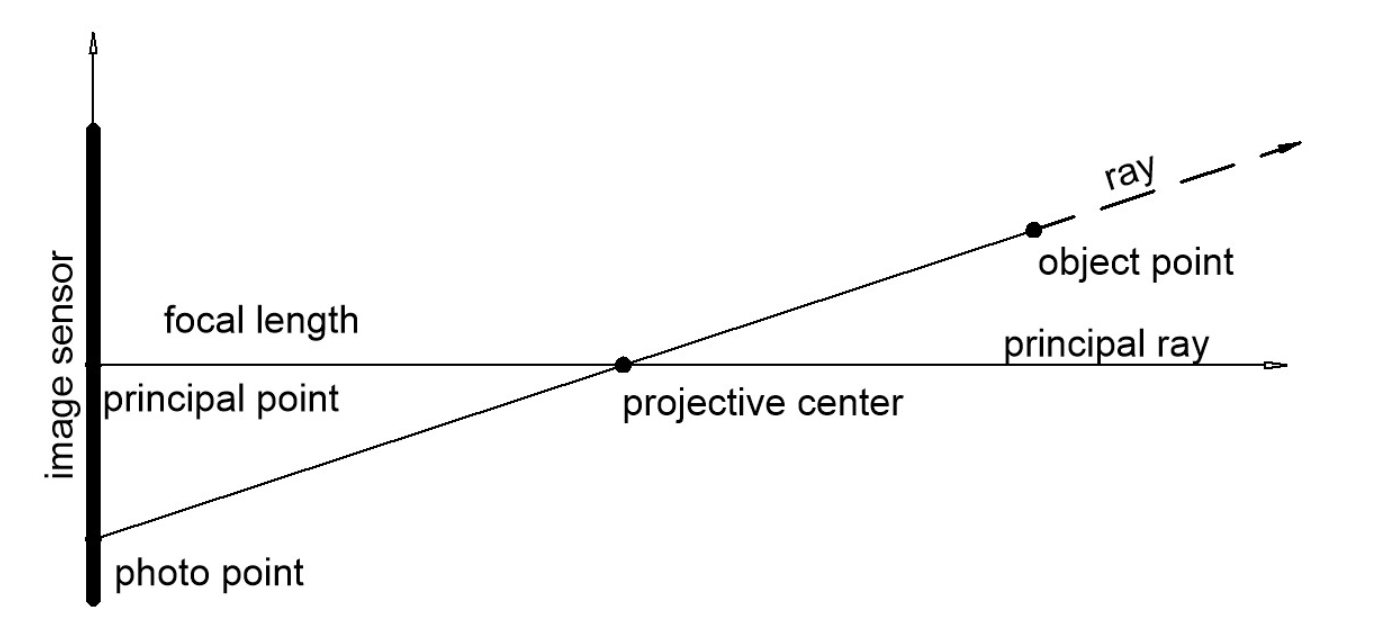
\includegraphics[scale=0.27]{figures/pinhole_camera.png}
    \caption{Pinhole camera model}
\end{figure}


\term{Image plane} is represented by a digital camera image sensor which  creates photo converting light into electronic signal.
Then the signal is processed inside a camera giving output in a form of photograph stored in a digital format. 
The image sensor is divided into cells measuring intensity of fallen light on their surface. A pixel value in final 
photograph is based on the measured intensity of cell or group of cells. The photo created by image sensor is inverted. This kind 
of photo is called \term{negative} in analog photography.  Usually the inversion is removed during processing inside a~camera. The resulting non inverted photo is called \term{positive} in analog photography. 

\begin{figure}[h]
    \centering
    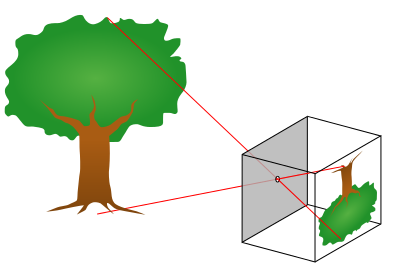
\includegraphics[scale=0.4]{figures/pinhole_camera_inversion.png}
    \caption{Pinhole camera photo inversion \cite{mellish2005pinhole}}
\end{figure}

% ML: \term{} na konci vety vytvari NEZADOUCI MEZERU, to se da
% odstranit v definici znakem '%'

%%% -> ML: OK (jiz opraveno)

All light \term{rays} going from object points and falling on an image sensor are going through the same point in the pinhole camera model.
The point is called \term{projective center}. The ray which is a perpendicular to the image sensor plane is called \term{principal ray} and the point 
where the principal ray intersects the image sensor plane is called \term{principal point}.

The pinhole camera model defines two coordinate systems. 2D  \term{photo coordinate system} is coincident
with the plane of positive.
The coordinates of photo point are expressed in this system. Another one is 3D \term{camera coordinate system}
where the object point is located. The system originates in projective center, Z coordinate 
 is coincident with a projective ray and X, Y axes are parallel to x, y axes of a photo system.

 
As a consequence of dimensional reduction caused by 
3D scene projection onto 2D plane, some information is lost.
If 3D coordinates of point are known, it is possible to reproject it on the image sensor plane. Because 
of the dimensional reduction, only a ray can be reconstructed from a 2D photo point.
3D coordinates of a point can not be determined.

In order to solve the ambiguity of object point position on the ray, additional information is needed.  
%%% ML: "a additional" asi bez clenu, jinak je spravne 'an'
%%% ST: opraveno
%%% -> ML: OK
It can be provided by another photo from different position capturing same point. 
If positions of photos 
 are known (this is called\term{ exterior orientation}), it is possible 
to reconstruct 3D coordinates of the point because it lies on the intersection of the photo rays.

%%% ML: predpokladam, ze obrazky bez uvedene reference jsou puvodni
%%% ST: Jj ale nekere jsou na zaklade inspirace z predlohy
%%% -> ML: v tomto pripade je vhodne uvest predlohu jako zdroj s poznamkou 'upraveno'
%%% -> ST: uvadim based on 

\begin{figure}[h]
    \centering
    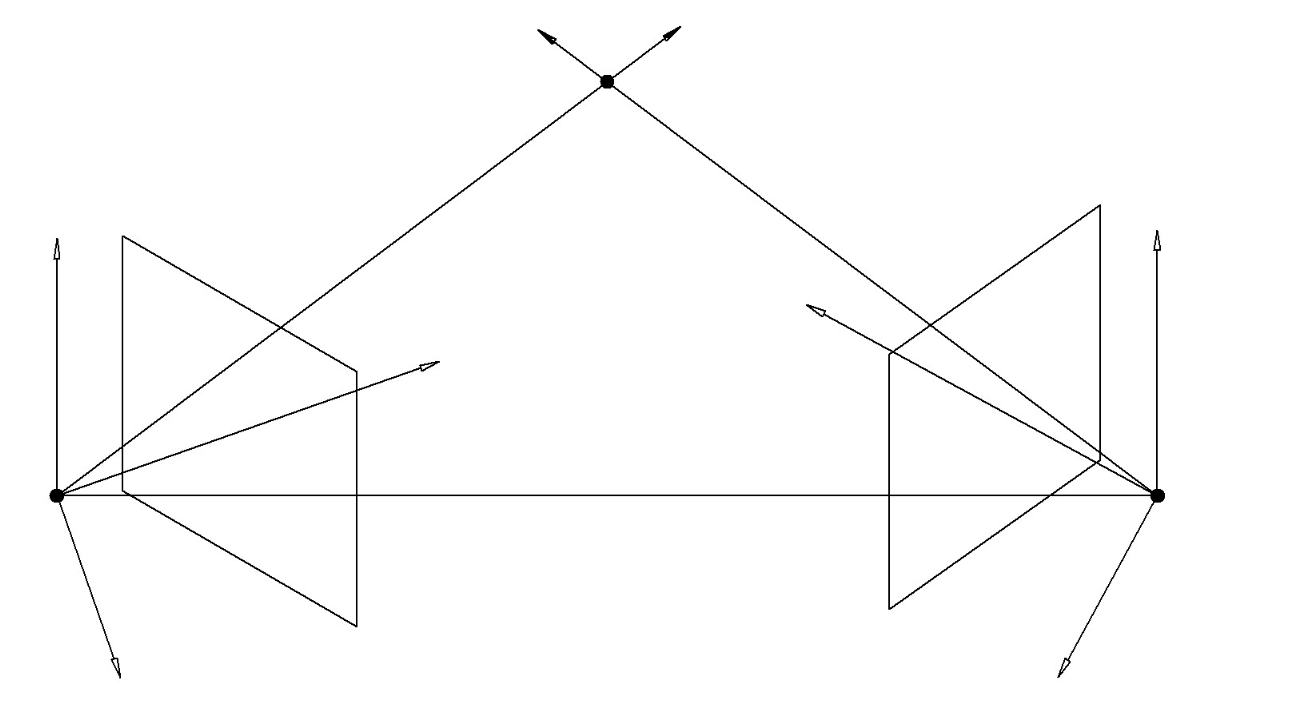
\includegraphics[scale=0.2]{figures/ray_intersection.png}
    \caption{Object point reconstruction from intersection of two photo rays.}
    \label{fig:obj_intersec}
\end{figure}

Real positions of the points and exterior orientation of cameras are expressed in \term{object coordinate system}. 
The exterior orientation describes relation between object coordinate system and camera coordinate system. 
The relation between point in the object 
space and point in the photo space can be expressed by combining interior and exterior orientation together.

In this thesis are introduced and used methods leading to retrieval of a scene structure from 
the set of photos which are based on such a simple principle of the ray intersection! Computer vision calls it \term{structure from motion}
and photogrammetry uses it for the creation of orthophoto, DTM or structure of object.

%%% ML: spravnejsi by bylo napsat DMT v kombinaci s ortofotem (drap
%%% over)
%%% ST: napsano
%%% -> ML: OK

\begin{figure}[h]
    \centering
    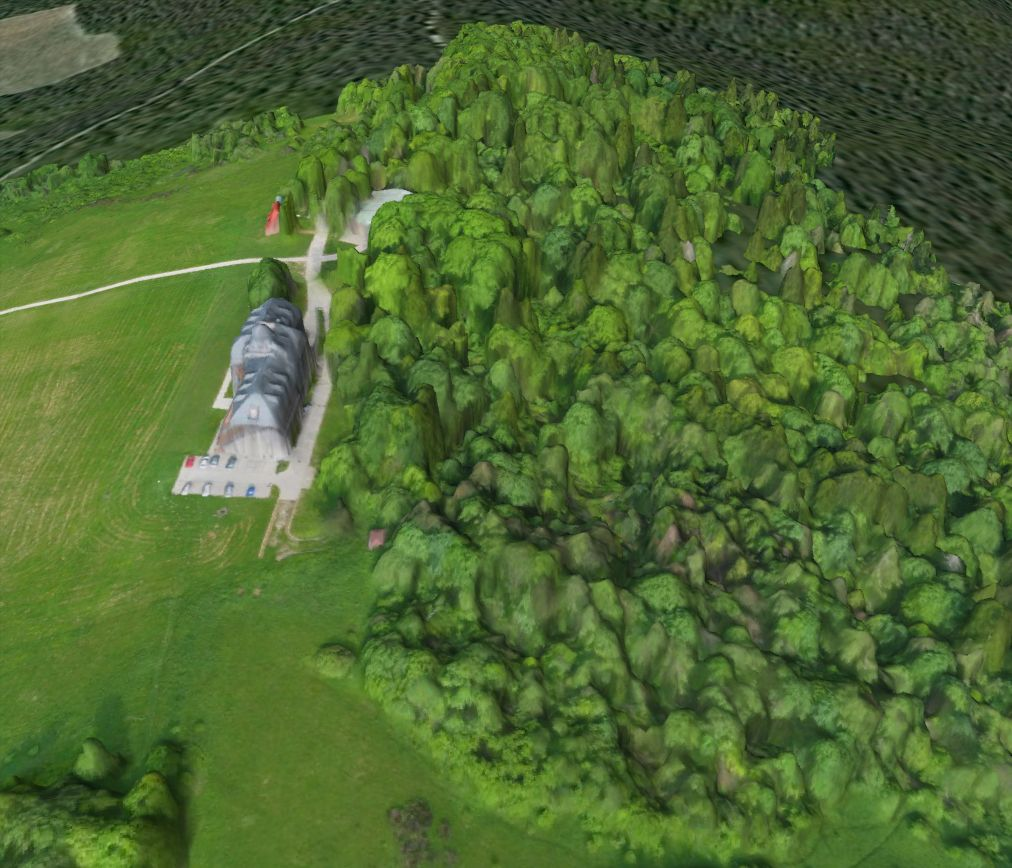
\includegraphics[scale=0.3]{figures/dtm.jpg}
    \caption{Digital terrain model overlaid with orthophoto \cite{kbosak2010bezmiechowa}.}
\end{figure}

%%% ML: misto Mapy.cz bych asi uvedl mezinarodni projekt anebo v
%%% poznamce pod carou vysvetlit co je Mapy.cz
%%% ST: zmeneno na bing
%%% -> ML: OK

Orthophoto is created in 
orthorectification process which means a transformation from perspective projection into orthogonal projection.
Unlike photographs, orthophotos can be merged together into seamless map. Recently, 
orthophoto has been widely used by some map services e.g. Google Maps or Bing Maps. Orthophoto 
has same scale in all parts therefore it is possible to measure true distances as in a~map. 
During orthorectification, distortion 
caused by tilt of camera (if photo is not vertical) and elevation differences are removed.

%%% ML: pokud je popisek obrazku moc dlouhy, tak by mel byt pro sekci
%%% 'seznam obrazku' zkracen \caption[kratky]{dlouhy}
%%% ST ma smysl vubec mit sekci seznam obrazku, nenapada me to duvod k cemu je to uzitecne

%%% -> ML: vetsinou se prikalada spolecene se seznamem tabulek (obcas
%%% se hodi pro prehled), ted to ale nech tak jak to je, tedy pouze se
%%% seznamem

\begin{figure}[h]
    \centering
    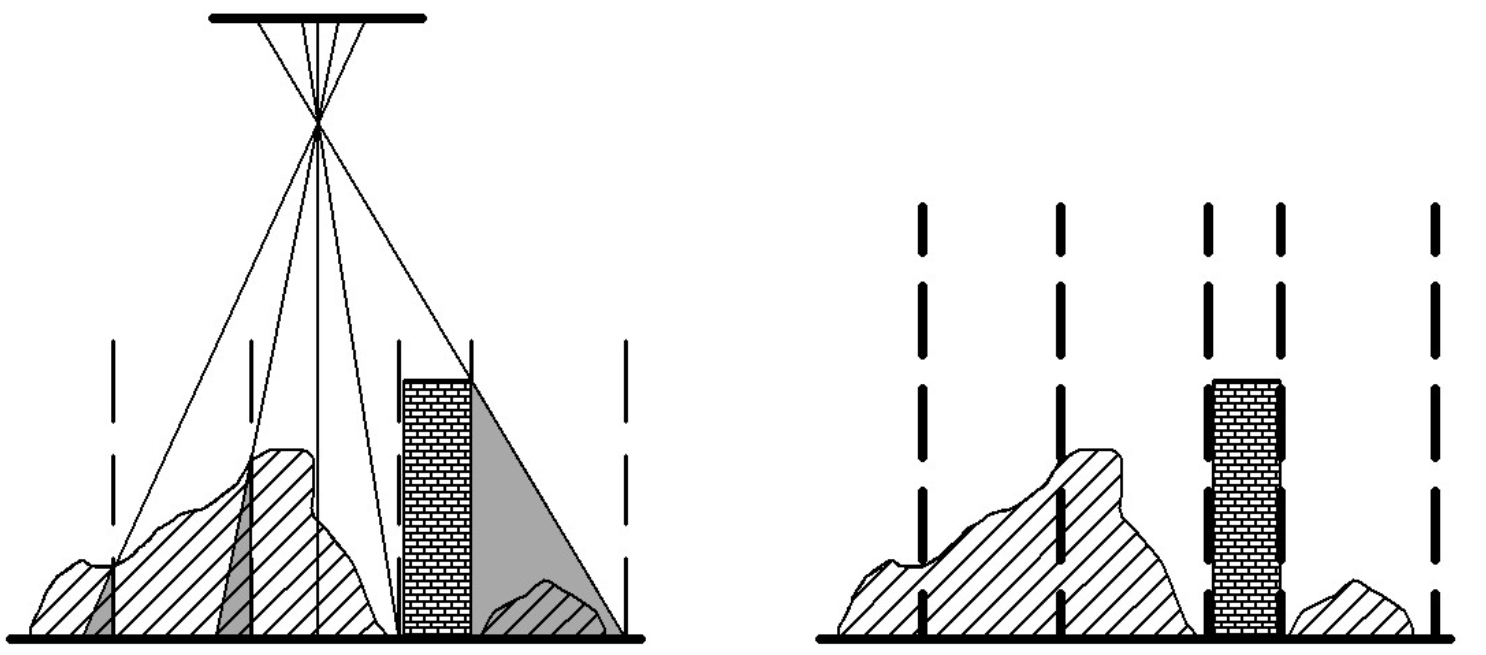
\includegraphics[scale=0.2]{figures/orthophoto.png}
    \caption{On the left side, there is clearly visible effect of elevation differences 
    caused by perspective projection of pinhole camera model. 
    In the right side, there is depicted orthogonal projection of orthophoto (based on \cite{pavelka2004foto20}[p. 151])}
    \label{fig:ortho}
\end{figure}


\subsection{GRASS GIS}
\label{sec:GRASS_intro}
%%% ML: hodila by se reference na GNU GPL a mozna i na webove stranky
%%% projektu GRASS
%%% ST: pridal jsem web grassu, GNU GPL je zminena jen tak na okraj...
%%% -> ML: OK
%%% -> ML: pouze na okraj - nemas vysvetlenu zkratku CERL (nevadi, tlaci nas cas)
%%% -> ST: pridana

GRASS (Geographic Resources Analysis Support System) \footnote{\url{http://grass.osgeo.org}} 
GIS is a free GIS software 
capable of processing raster, vector and imagery data. 
GRASS belongs among one of 
the longest active software projects. Development of GRASS was begun by the U.S. Army CERL laboratory (Construction Engineering Research Lab)
in the first half of 1980s. In 1990s, U.S. Army gradually ceased developing GRASS. Luckily, 
the development could be taken over by volunteers because
it had been decided to release its source code as public domain.  License 
of GRASS was changed into GNU GPL v2 in 1999. GRASS is developed by the GRASS Development 
Team comprised of developers spread world wide. 

%%% ML: reference na QGIS a ArcGIS nebo jako poznamka pod carou (?)
%%% ST: uvadet je vubec? je to poznamemanano na okraj, a adresu si kazdy najde v googlu, 
%%% podle mne poznaka pod carou jen zabira misto
%%% -> ML: OK
%%% ML: "a new users", bez clenu nebo "the new users" (?)
%%% ST: opraveno

%%% -> ML: nerozumim uplne co znamena "graphical user interface which
%%% has evolved dynamically", ale to nevadi
%%% -> ST: prepsano

Individual functionalities of GRASS are implemented in form of small software packages called modules which 
can be combined together to solve complex tasks.
Unlike other GIS systems as QGIS or ArcGIS, it takes 
more time for a new user to start understand the GRASS philosophy.  Developers 
have been aware of this problem therefore they decided to develop a graphical user interface
making GRASS more friendly for beginners.

%%% ML: "so called" GIS database (?)
%%% ST: ok

Data in GRASS are stored in so called  \term{GIS database} composed of \term{locations}. Every location 
defines its projection thus all data belonging to the location must be reprojected to it. 
The location comprises \term{mapsets} used for organization 
of the data into consistent units. 

%%% ML: pro citelnost textu by mozna bylo dobre slova location, mapset
%%% ci comp. region pri prvnim pouziti zvyraznit ({\em }) - osobni
%%% nazor (low priority)
%%% ST: zvyrazneno

%%% ML: nektere moduly pro praci s vektorovymi daty maji prepinar pro
%%% akcepovani regionu, ale zde bych to neuvadel, neni to pro praci
%%% dulezite
%%% ST: smazano
%%% -> ML: OK
%%% ML: extend -> extent (jiz opraveno, snad jsem nic neprehlednul)

Another important element of GRASS is a \term{computational region}. The region stores information about a geographical
extent defined by four values (north, south, east, west) of a bounding box and 
another two values representing south-north and west-east resolution. Properly set region is 
very important for raster data processing because nearly all raster modules performs computation 
on currently set region. Only exception are import raster modules ignoring it by default.


\subsection{UAV}
\label{sec:UAV_intro}
%%% ML: myslim, ze se nejvic UAV vyrabi v Izraeli, pouziti pro
%%% vojenske ucely je nejvice viditelne u U.S. Army, ta Izraelska je
%%% snad pouziva jeste vic, to jenom na okraj

An unmanned aerial vehicle (UAV also known as drone) is aircraft without human pilot.  UAVs have been ingloriously known for
 heavy military employment especially by USA in Afghanistan and Pakistan. These military drones are equipped with state of the art 
technology and their construction is similarly complex as a small aircraft.  
A number of military UAVs is quickly raising and nowadays USA trains more UAV operators than fighter plane pilots.

%%% ML: prize -> price (jiz opraveno)

Besides military UAVs, the sector of civil drones is exponentially growing. It is very broad category ranging
from big military like drones to small ones in size of a few decimeters. There are several types of drones e.g. airplanes,
helicopters, multicopters, paraglides, airships, balloons and others. 
The promising category of drones are multirotor drones (e.g. hexacopters or octocopters) because they have simple construction and 
even ordinary users are able to learn control them very quickly. Because of steeply falling prices of the octocopters, it can be expected 
that this kind of drone will become commonly used for many civil purposes.

In photogrammetry, cheap civil UAVs can be successfully employed in the mapping missions for creation of DTM/structure or orthophoto.
The main advantage of a UAV mapping mission is cost saving compared to a mission performed by manned aircraft.
In order to obtain photos of desired area, camera is mounted on UAV. During the UAV flight, photos of the mapped 
area are taken with sufficient overlap (usually at least 60 percent). The overlap of photos is used for identification 
of corresponding photo points whose 3D object coordinates are obtained by intersection of rays (see \ref{sec:ess_princip}). 

\begin{figure}[h]
    \centering
    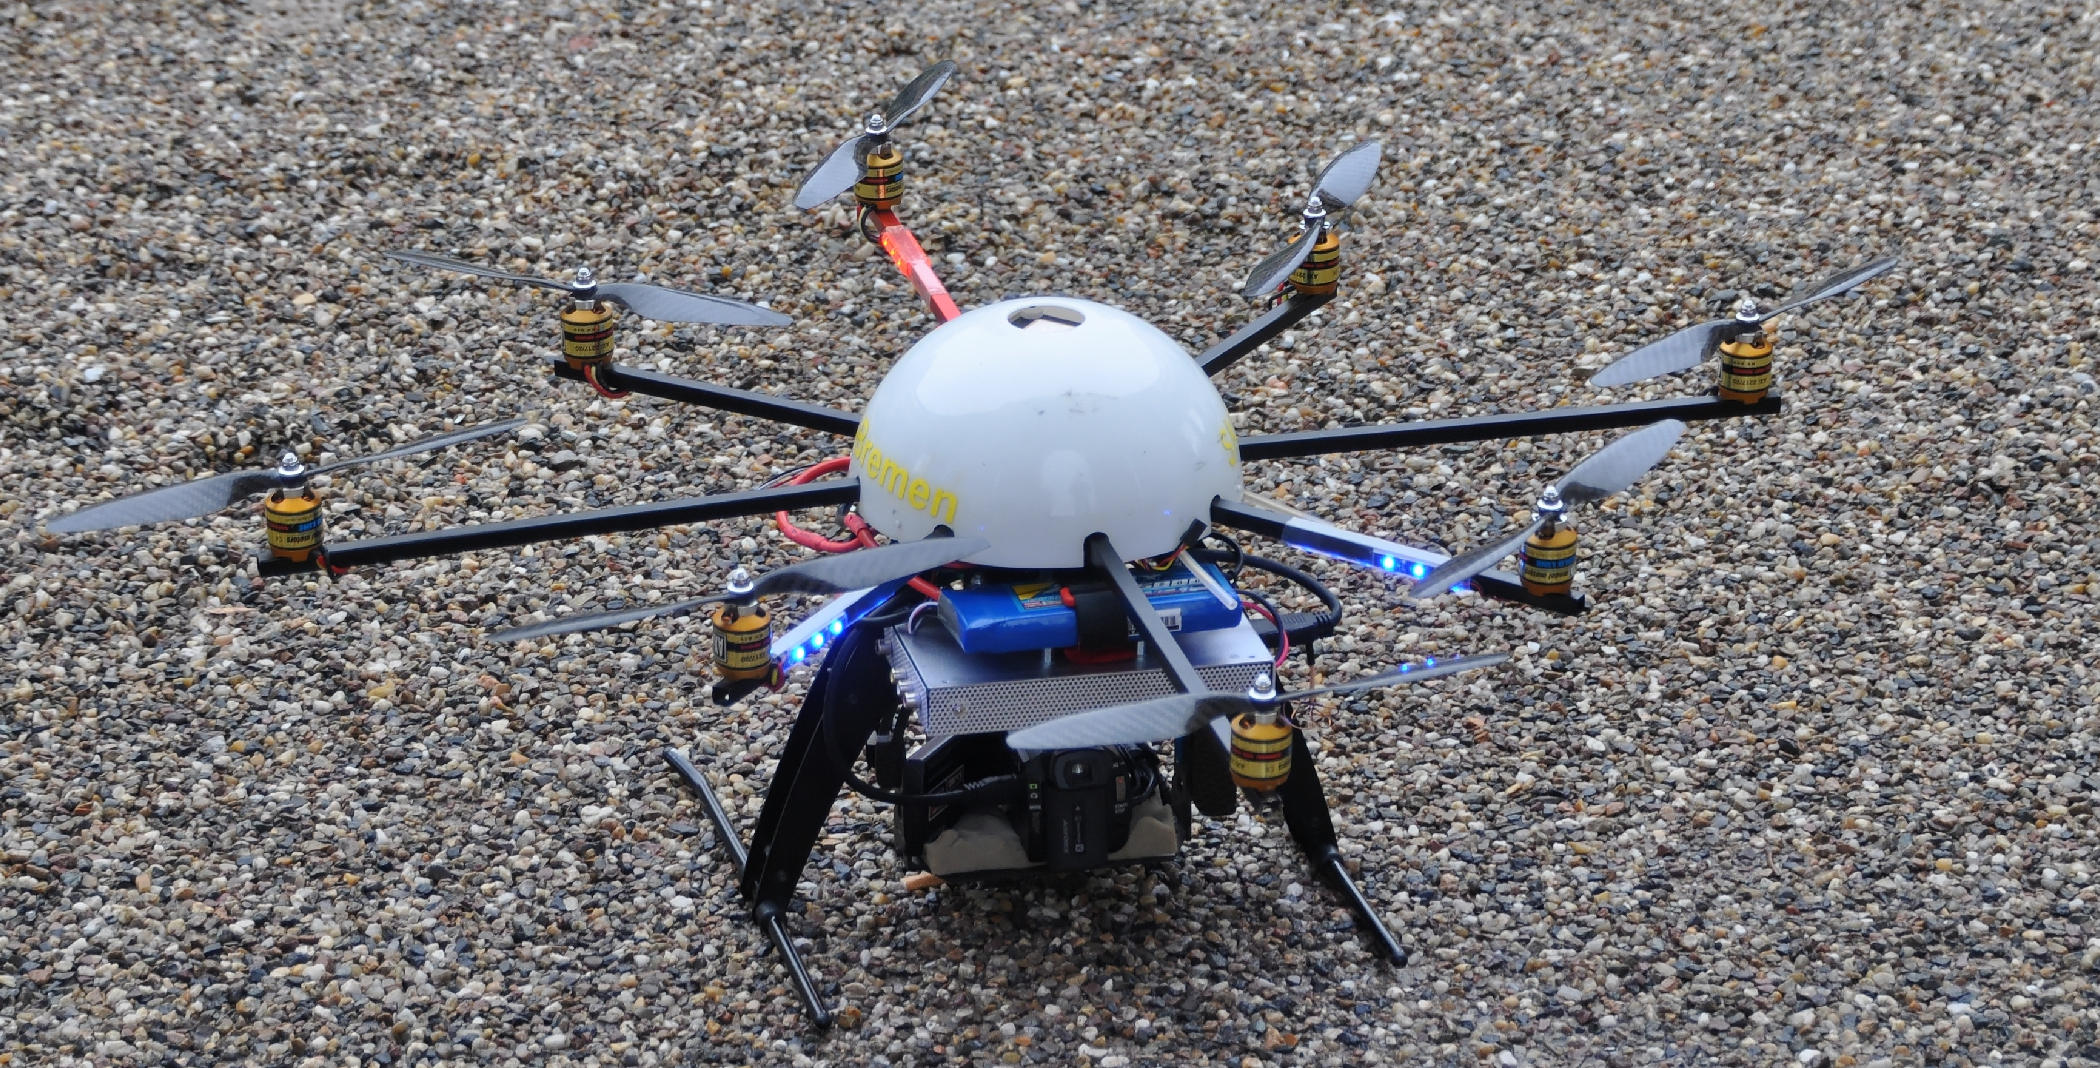
\includegraphics[scale=0.8]{figures/octocopter.jpg}
    \caption{An octocopter \cite{boe2013octocopter}}
    \label{fig:sample_figure}
\end{figure}

%%% ML: pred finalnim tiskem zkontrolovat rozumne pozicovani obrazku a
%%% hlavne zacatek kapitoli na konci stranky, da se vyresit zvetseni
%%% mezery (\vskip) anebo vynucenim konce stranky (\newline)
%%% -> ML: OK

\subsection{Least squares}
\label{sec:least}

%%% ML: v kapitole nejsou uvedeny ZADNE reference, nepredpokladam, ze
%%% jsi ji psal z patra bez pouziiti zadne literatury...
%%% ST: pridal jsem 6 referenci 
%%% -> ML: OK

In linear algebra, commonly solved equation is:

\begin{equation}
\label{eq:linear_eq}
\ematr{A}\evect{X} = \evect{L} 
\end{equation} 


%%% ML: \evect{} podobny problem jako u \term{} - VYNUCENA MEZERA, coz
%%% dela neplechu na konci radky (mezera pred teckou), podobnym
%%% problem budou trpet i dalsi prikazy, chtelo by je opravit
%%% (%) a zkontrolovat, zda nekde mezera naopak nechybi

%%% -> ML: OK (jiz opraveno vcetne mezery pred terminem)

\noindent It can be interpreted as:
\begin{itemize}
\item \evect{L} - a vector of measurements,
\item \evect{X} - a vector of unknown parameters whose values are searched to solve \eqref{eq:linear_eq},
\item \ematr{A} - a matrix of a linear cost functions coefficients  where row represents one measurement
		  and column represents one parameter of cost function. Linear cost functions $\efunc{f_{i}(\evect{X})}$
		  represent relationship between measurements \evect{L} and searched parameters \evect{X}. 
		  Least square method calls it a \term{design matrix}. 
\end{itemize}

%%% ML: prvni veta zni divne...
%%% ST: snad lepsi

%%% -> ML: OK

There is exactly one solution 
of vector of parameters  \evect{X} to satisfy the equation if matrix \ematr{A} is 
non singular matrix  and vector \evect{b} is not a zero vector. Non singular matrix is always square matrix
which has all column vectors and row vectors linearly independent. 

%%% ML: zvyraznit jednotlive polozky (?), napr. {\em gross error}
%%% ST: zvyrazneno 
%%% -> ML: OK

Basically, every measurement is burden with some error. Errors can be divided into these main categories:  
\begin{itemize}
\item \term{gross error} - it is caused by human factor or fault of the instrument. If the measurement is repeated,
usually, it is possible to identify measurements influenced by this error because 
they are big outliers from the other measurements unaffected by this 
kind of error.
\item \term{systematic error} - if measurement is repeated by the same instrument,
it has same effect (value) on the measurement.  Usually effect of this error can be 
eliminated by choosing right measurement method, calibration of the instrument or taking it into account in a mathematic model.
\item \term{random error} - this error is unavoidable because it is impossible to know perfectly all factors which has impact 
on a measurement. The random errors follow normal distribution represented by probability density function of this shape.

%%% ML: TODO
%%% ST: obrazek pridan

\begin{figure}[h]
    \centering
   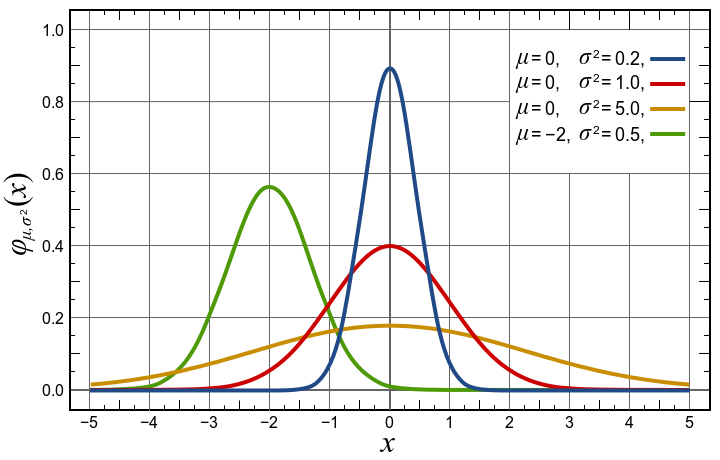
\includegraphics[scale=0.4]{figures/normal_dist.png}
    \caption{Density functions of normal distributions depending on values of standard deviation 
$\escal{\sigma}$ and mean $\escal{\mu}$ \cite{inductiveload2008selection}}
    \label{fig:norm_dist}
\end{figure}

%%% -> ML: zde jsem pridal par clenu, snad k lepsimu...

The normal distribution is characterized by two parameters which are \term{standard deviation}
$\escal{\sigma}$ and \term{mean} $\escal{\mu}$. 
If measurements are burden only with random error, the mean represents accurate value and standard deviation represents 
dispersion level of measurements. 
Theoretically,  if the measurements of some parameter would be repeated infinite times and the measurements would be influenced only by random errors,
accurate values could be computed as a~mean.
It follows that it is possible to get closer to the accurate value by repetition of measurements
leading into solving overdetermined systems. Another important implication 
is that the mean of the measurements performed by a more accurate 
instrument is statistically closer to the accurate value than the mean of same number of the measurements performed
by a less precise instrument.
Measurements of different accuracies can be combined together by weighted mean
with weight of measurement $\escal{p}_{i}$ defined as:
\begin{equation}
\label{eq:wmean}
\escal{p}_{i} = \frac{\escal{const}}{\escal{\sigma}_{i}^{2}}
\end{equation} 
where \escal{const} is arbitrary chosen number used for calculation of all weights 
and $\escal{\sigma_{i}}$ is standard deviation of an instrument (representing accuracy) used for the measurement.
\end{itemize}

The overdetermined systems are solved in many fields where final accuracy of determined 
quantities by measurement (e.g. 
surveying, photogrammetry etc.) matters.

%%% -> ML: zde jsem odstranil jednu z referenci (\eqref{eq:linear_eq})

As the consequence of overdetermination, the design matrix \ematr{A} becomes rectangular with more rows than columns 
and therefore the solution for linear equations system \eqref{eq:linear_eq} does not exist.
Only if the measurements were perfect it would be possible to find such parameters vector \evect{X} to 
solve the system of the linear equations. 

%%% -> ML: tady mluvis o 'cost functions' ale v predchozim textu nemas
%%% vysvetlono o co jde
%%% -> ST: je vysvetlena v uvodu hned pod prvni rovnici 

Due to measurement imperfections, it is not possible to find such parameters of vector \evect{X} to make difference
\evect{v} between measured values and results of cost functions using  parameters vector equal to zero:

\begin{equation}
\label{eq:least_v}
\evect{v} = \evect{L} - \ematr{A}\evect{X}
\end{equation} 

Hence, it is needed to define another condition allowing to find optimal solution of the 
overdetermined system.

\begin{figure}[h]
    \centering
    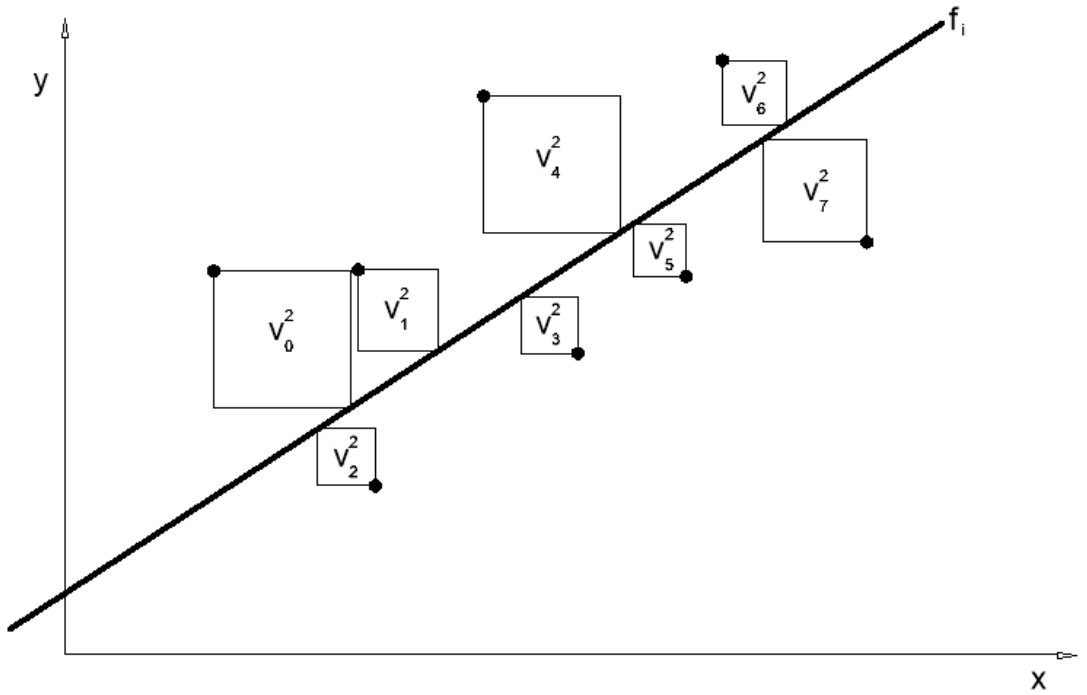
\includegraphics[scale=0.27]{figures/squares.png}
    \caption{In this case least squares method finds a line
    which minimizes sum of areas of squares. }
    \label{fig:squares}
\end{figure}

The least squares method finds values of parameters vector \evect{X} 
following condition minimizing sum of the squares of differences \evect{v} (see Figure \ref{fig:squares}): 

\begin{equation}
\evect{v}^{T} \evect{v} = min
\end{equation} 

The minimized square differences equation can be rewritten as:

\begin{equation}
\begin{split}
\evect{v}^{T} \evect{v} &= (\evect{L} - \ematr{A}\ematr{X})^{T} (\evect{L} - \ematr{A}\ematr{X}) \\
&= \evect{L}^{T} \evect{L} - 2 \evect{L}^{T} \ematr{A} \evect{X} + \evect{X}^{T} \ematr{A}^{T} \ematr{A} \evect{X}
\label{eq:least_be_part}
\end{split}
\end{equation} 

According to calculus notation, the least squares method searches for global minimum of the square differences equation. 
The global minimum of a function can be obtained using partial derivative of parameters in the cost function.
In case of linear cost functions,  
their square forms  second degree polynomial e.g. parabola in \eucl{2}, paraboloid in \eucl{3} etc. All these functions has
only one point where all partial derivatives are equal to zero regardless dimension of the function. It is 
exactly the global minimum which the least squares method searches for!

The partial derivative of the minimized square differences equation can be written as \cite{mathematicalfrederico}:
 
\begin{equation}
\frac{\partial \efunc{f} (\evect{v}^{T} \evect{v}) }{\partial \evect{X}} = -2\ematr{A}^{T} \evect{L} + -2\ematr{A}^{T}\ematr{A} \evect{X} 
\label{eq:least_part}
\end{equation} 

The global minimum can be find by giving this equation equal to zero:
\begin{equation}
-2\ematr{A}^{T} \evect{L} + -2\ematr{A}^{T}\ematr{A} \evect{X} = 0 
\end{equation} 

The least square determines values of parameters vector \evect{X} which can be expressed from the previous equation:
\begin{equation}
\evect{X} = (\ematr{A}^{T} \ematr{A})^{-1} \ematr{A}^{T} \ematr{L}
\end{equation}

It is essential equation of the least squares method. The equation can be solved simply by means of linear algebra.

The equation supposes that all measurements have same weight (accuracy). The least squares method can be extended to support weights.
Weight matrix \ematr{P} contains weights of measurements on the diagonal with off-diagonal being zero elements if
the measurements are not correlated.

The equation minimized by least squares is extended by the weight matrix into following form:
\begin{equation}
\evect{v}^{T}  \ematr{P} \evect{v} = min
\end{equation}

Therefore, the essential least square equation is altered into this form:
\begin{equation}
\label{eq:least_sq}
\evect{X} = (\ematr{A}^{T} \ematr{P} \ematr{A})^{-1} \ematr{A}^{T} \ematr{P} \ematr{L}
\end{equation}

\subsubsection{Non-linear least squares}
\label{sec:non_least}
So far, it was supposed that the cost function is linear thus global minimum can be found simply by means of linear algebra  \eqref{eq:least_sq}.
Unfortunately, it is common that the relationship between parameters and 
measured values is not linear, hence, it is needed to adapt linear least squares equations for non-linear
cost functions.

Unlike linear least squares whose square of difference \eqref{eq:least_be_part}
is represented by function  (parabola, paraboloid...) with just one point where all
partial derivatives are zero, the non-linear cost function can have many such points e.g. other local minimas. 

The problem of non-linearity can be solved by linearization of non-linear equations.
The main idea of linearization process is to approximate the cost function with first degree Taylor polynomial,
which is linear. Therefore, it is possible to use linear least square equation \eqref{eq:least_sq} 
to solve non-linear problem. 

\begin{figure}[h]
    \centering
    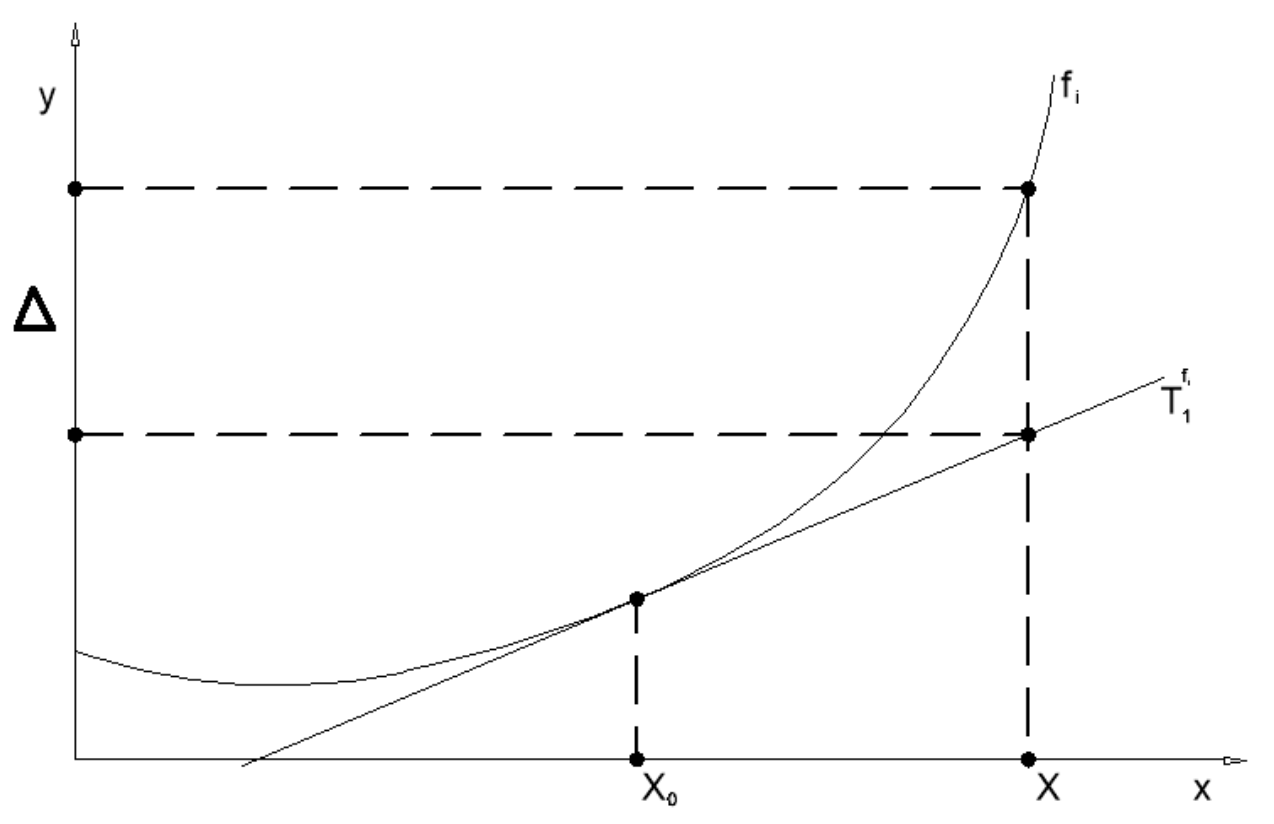
\includegraphics[scale=0.2]{figures/taylor.png}
    \caption{Function $\efunc{f}_{i}$ is approximated by first degree Taylor polynomial $\efunc{T} ^{\efunc{f}_{i}}$,
     forming line in \eucl{2}. Symbol $\Delta$ represents an approximation error.}
    \label{fig:taylor}
\end{figure}


Approximation of the cost function by a first degree Taylor polynomial can be written as \cite{cadaprednaskove}:
\begin{equation}
\efunc{T} ^{\efunc{f}_{i}, \evect{X}_{0}}_{1} (\evect{X}) = 
	      \efunc{f}_{i}(\evect{X}_{0}) + 
               \frac{\partial}{\partial {\escal{X}_{0_{1}}}} \efunc{f}_{i} (\evect{X}_{0}) (\evect{X} -  \evect{X}_{0}) 
\ ... \ + \frac{\partial}{\partial {\escal{X}_{0_{n}}}} \efunc{f_{i}}(\evect{X}_{n}) (\evect{X} - \evect{X}_{0}) 
\end{equation}

%%% ML: pozor na konec stranky (projit az na konci pred finalnim
%%% tiskem)

%%% ML: nemel by to byt clen? "is a point"
%%% ST: jj mel

\noindent where:
\begin{itemize}
\item $\evect{X}_{0}$ is a point where the Taylor polynomial touches approximated function. 
      For instance, first degree Taylor polynomial 
      is a line which is a tangent of function at the point $X_{0}$ in \eucl{2}, tangent plane in \eucl{3} and  
       tangent hyperplane in  \eucl{n}.
\item \evect{X} is a point where the Taylor polynomial returns approximate value of the cost function $\efunc{f}_{i}$.
\end{itemize}

Least squares Taylor polynomial can be written as:

\begin{equation}
\efunc{T} ^{\efunc{f}_{i}, \evect{X}_{0}}_{1} (\evect{X}) =  \efunc{f}_{i}(\evect{X}_{0}) + \escal{a}_{0} \escal{dx}_{0} \ ... \ + \escal{a}_{n} \escal{dx}_{n} 
\end{equation} 

It can be rewritten into a matrix form with formal substitution $\evect{L_{X_{0}}} = \efunc{f}_{i}(\evect{X}_{0})$:
\begin{equation}
\label{eq:expanded_taylor}
\efunc{T} ^{\efunc{f}_{i}, \evect{X}_{0}}_{1} (\evect{X}) = \evect{L_{X_{0}}} + \ematr{A}\evect{dx}
\end{equation} 

It should be noted that the design matrix \ematr{A} contains partial derivatives of cost functions. 
Analogous equation to \eqref{eq:least_v} can be derived:
\begin{equation}
\evect{v} = \evect{L} - \efunc{T} ^{\efunc{f}_{i}, \evect{X}_{0}}_{1} (\evect{X})
\end{equation} 
 
Taylor polynomial member can be expanded by \eqref{eq:expanded_taylor}:
\begin{equation}
\begin{split}
\evect{v} &=  \evect{L_{X_{0}}} - \evect{L} - \ematr{A}\evect{dx} \\
          &= \evect{l} - \ematr{A}\evect{dx}
\end{split}
\end{equation}

If the differences vector from the previous equation is substituted into least squares minimization criterion:
\begin{equation}
\label{eq:min_cond}
\evect{v}^{T}  \ematr{P} \evect{v} = min
\end{equation}

The essential equation for non linear least squares can be derived 
similarly to linear least squares:

\begin{equation}
\begin{split}
\label{eq:non_least_sq}
\evect{dx} &= (\ematr{A}^{T} \ematr{P} \ematr{A})^{-1} \ematr{A}^{T} \ematr{P} \ematr{l} \\
\evect{X} &=  {\evect{dx} -  \evect{X_{0}}} \\
\end{split}
\end{equation}

%%% ML: prize -> price (jiz opraveno)

The equation is slightly different compared to the linear least squares equation \eqref{eq:least_sq}.
 Instead of the parameters vector \evect{X}, result of the equation is 
 correction vector  of parameters \evect{dx}. Measurement vector \evect{L} is analogous to vector \evect{l}. In this two minor 
substitutions, there are hidden major limitations of the non-linear least squares method 
where the price for the approximation is paid. 

%%% -> ML: "the Taylor polynomial requires some point $\evect{X_{0}}$
%%% where it is tangent to approximated function." tohle zni divne
%%% formulovano
%%% ST prepsano

As it was already mentioned, the Taylor polynomial is tangent of approximated at point $\evect{X_{0}}$.
This approximation is good in close surroundings of the point $\evect{X_{0}}$, however, as the distance 
grows, the approximation error $\Delta$ may increase significantly which can be clearly seen in Figure \ref{fig:taylor}.

Therefore, unlike linear least square method, non-linear least squares requires initial 
values of parameters \evect{X}. If the initial values are not accurate 
enough, it is possible to iteratively run linear least squares subsequently.
In the new iteration, adjusted parameters vector \evect{X}
from the previous iteration is used to eventually approach global minimum of the cost function. 
Therefore the closeness of the initial point $\evect{X_{0}}$ to global minimum affects how many iterations (speed of convergence)
are needed to achieve optimal solution (global minimum).

Unfortunately, the non-linear least square method has another one, even more serious pitfall which 
does not guarantee that it will iterate towards global minimum at all!
In such a case, the found values of parameters vector \evect{X} are completely wrong because 
it does not satisfies minimum squares difference condition \eqref{eq:min_cond}. If the initial values are 
inaccurate, the method can iterate toward other points with zero derivation (e.g. local minimums).  
This is caused by run-off of minimized function created from non-linear cost function which can have more points with zero derivative
unlike the minimized function by linear least squares method.

Therefore, success of non-linear least squares method depends on the initial values of parameters vector $\evect{X}$!

\subsubsection{Least squares properties}

It was proved \cite{mervart2007adjustment} that above derived least square method is solution of Gauss-Markoff model which says:
If measurements \evect{L} are random with known covariance matrix $\ematr{\Sigma}_{l}$  
and vector of unknown parameters \evect{X} is non-random then
vector \evect{dx}  has the lowest variance and it is unbiased. If density functions of measurements are normally 
distributed (see Figure \ref{fig:norm_dist}) then values obtained from the cost functions using  computed parameters lies in maximum of the density
function. In other words, they posses maximum likelihood.

The weight matrix is calculated from covariance matrix in similar way as weights in weighted mean \eqref{eq:wmean}:
\begin{equation}
\ematr{P} = \frac{\escal{const}}{\escal{\Sigma}_{i}^{2}}
\end{equation} 

Where \escal{const} is chosen arbitrary. It can be selected as a priori standard deviation of unit weight $\sigma_{0}$. 


Unbiased unit weight standard deviation $\hat{\sigma}_{0}$ can be also estimated a posteriori as:
\begin{equation}
\escal{\hat{\sigma}}_{0}^{2} = \frac{\evect{v}^{T} \ematr{P}  \evect{v}}{\escal{r}}
\end{equation} 

Where \escal{r} is redundancy which is difference of columns number from rows number of design matrix \ematr{A}.

Covariance of calculated parameters $\ematr{\Sigma}_{x}$ can be get from:
\begin{equation}
\ematr{\Sigma}_{\hat{x}} = \escal{\hat{\sigma}}_{0}^{2} (\ematr{A}^{T} \ematr{P} \ematr{A})^{-1}
\end{equation} 

A posteriori covariance matrix $\ematr{\Sigma}_{\hat{l}}$ of measurements can be obtained from:
\begin{equation}
\ematr{\Sigma}_{\hat{l}} =  \ematr{A} \ematr{\Sigma}_{\hat{x}} \ematr{A}^{T}
\end{equation} 

\subsubsection{Iteration termination}
\label{sec:term_crit}
Non-linear least squares method is iterative, thus it is needed define 
some criteria allowing to assess whether global minimum was reached. 

The criterion \cite{mikhail1976observations} can be 
based on assessment of parameters corrections \evect{dx}. 
For instance, it can be chosen threshold of maximum absolute value
of correction. If the threshold is not satisfied another 
iteration is performed. 

Another criterion is maximum number of iterations.
The criterion is important in cases when the least squares method
is unable to converge to some point resulting 
in impossibility to satisfy the previous criterion.

Thus, this criterion prevents from falling into infinite loop.
The threshold can not be chosen too small in order to
least squares method has enough iteration to converge to
global minimum. 


\subsubsection{Free network least squares}
\label{sec:free_net_least}

%%% ML: "datum deficiency" by chtelo zvyraznit (\em) - pouze osobni nazor
%%% ST:zvyrazneno

In geodesy, it can happen that columns of design matrix \ematr{A}
are not linearly independent. It can be caused by \term{datum deficiency} \cite{deakin2006rank}. 
The datum deficiency is missing information
about  coordinate system of the network in the design matrix \cite{strang1997linear}.
It makes \term{normal matrix} $ \ematr{A}^{T} \ematr{P} \ematr{A}$ non invertible because 
of linearly dependent columns of design matrix. 
Thus,
the least squares equation \eqref{eq:non_least_sq} can not be solved.
In order to avoid the datum deficiency issue, it is needed to keep some parameters fixed
which means that columns of the fixed parameters are excluded from design matrix \ematr{A}.

Photogrammetry deals with three dimensional space requiring at least  
two points to be fixed with another point with one coordinate to avoid datum deficiency problem because
three dimensional coordinate system is defined by three coordinates of shift vector, three rotation angles and scale factor. 

If there are not enough fixed points, a network has to be adjusted as a free network.
One of possible methods how to adjust a free network is calculation of pseudo inverse matrix of the normal matrix instead of
inverse. Another option is adding inner constraints to the least squares system.

\subsection{Short introduction to photogrammetry}

Essential information which must be known to obtain any photogrammetric
 product (e.g. orthophoto or DTM) from group of the photos is their interior orientation and exterior orientation.
Exterior and interior orientation together describe relation between a 3D object point and
corresponding 2D photo point.

\subsubsection{Interior orientation}

Interior orientation describes relation between photo coordinate system 
and corresponding 3D camera-related coordinate system which is based on pinhole camera model described in the chapter \ref{sec:ess_princip}.

Photogrammetric camera coordinate system has origin in projective point,
$z$ axis heading out of the scene  and $x$, $y$ axes being parallel to the photo plane. Directions of 
$x$, $y$ axes are selected in way to be the camera system right handed.

\begin{figure}[h]
    \centering
    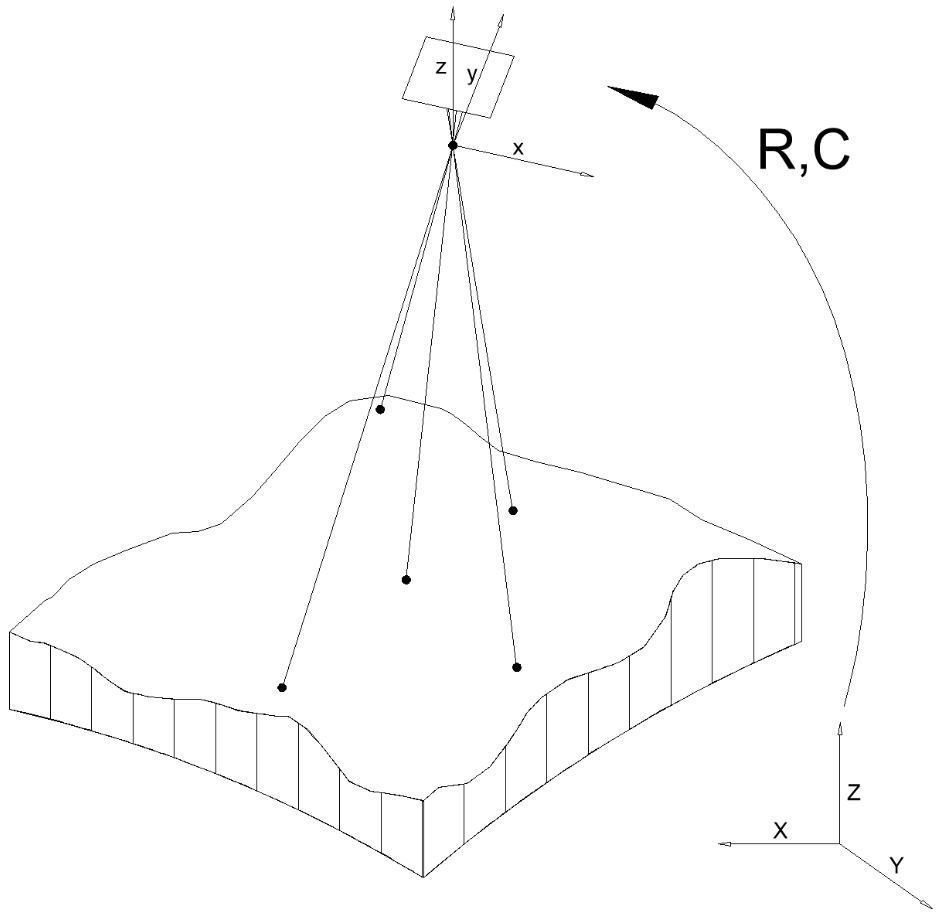
\includegraphics[scale=0.3]{figures/photogrammetric_model.png}
    \caption{Photogrammetric camera coordinate system in arbitrary object coordinate system.
    Rotation matrix \ematr{R} and vector \ematr{C} of projective center object coordinates represent 
    an exterior orientation. The \escal{x}, \escal{y}, \escal{z} represents axes of photogrammetric camera system and 
     \escal{X}, \escal{Y}, \escal{Z} are axes of the arbitrary object system.}
    \label{fig:ph_model}
\end{figure}

\noindent The interior orientation parameters describing pinhole camera model are:
\begin{itemize}
  \item Focal length \escal{f} -- a distance of projective center from the principal point,
  \item Principal point coordinates $(\escal{x}^{ph}_{pp}, \escal{y}^{ph}_{pp})$ -- in ideal case position of the principal point would be exactly in the middle 
	of a photo.  In most cases, there is some shift of the principal point from the photo center due to
	camera construction inaccuracies.
\end{itemize}

Camera optical system is imperfect therefore it deviates from the ideal pinhole model which 
 causes distortion of a photo.
The effect of distortion can be reduced by applying distortion corrections. Commonly 
used model for distortion is the Browns model \cite{brown1966distortion}.
The model defines following types of distortion:
\begin{itemize}
  \item \term{Radial distortion} -- it depends on distance from the principal point. Cause of the distortion is spherical shape of the 
  lens in camera optical system.
  \item \term{Tangential distortion} -- it is perpendicular to direction of radial distortion. It is caused by 
       imperfect alignment of lenses in camera optical system.
\end{itemize}

Mathematically the Brown model is expressed by these equations:

\begin{equation}
\label{eq:undistort}
\begin{split}
\escal{x}^{u} =& (\escal{x}^{ph} - \escal{x}^{ph}_{pp})(1 + \escal{K}_{1}r^2 + \escal{K}_2r^4 + ...) + \\
&(\escal{P}_1(\escal{r}^2 + 2(\escal{x}^{ph} - \escal{x}^{ph}_{pp})^2) + 2\escal{P}_2(\escal{x}^{ph} - \escal{x}^{ph}_{pp})(\escal{y}^{ph} - \escal{y}^{ph}_{pp}))(1 + \escal{P}_3r^2 + \escal{P}_4r^4 ...) \\
\escal{y}^{u} =& (\escal{y}^{ph} - \escal{y}^{ph}_{pp})(1 + \escal{K}_1r^2 + \escal{K}_2r^4 + ...) + \\
&(\escal{P}_2(\escal{r}^2 + 2(\escal{y}^{ph} - \escal{y}^{ph}_{pp})^2) + 2\escal{P}_1(\escal{x}^{ph} - \escal{x}^{pp})(y^{ph} - \escal{y}^{ph}_{pp}))(1 + \escal{P}_3r^2 + \escal{P}_4r^4 ...) \\
\escal{r} =& \sqrt{(\escal{x}^{ph} - \escal{x}^{ph}_{pp})^2 + (\escal{y}^{ph} - \escal{y}^{ph}_{pp})^2}
\end{split}
\end{equation}

\noindent where:

%%% ML: jednotlive polozky se vetsinou oddeluji carkou a posledni
%%% konci teckou (zde opraveno, nevim jak jinde v textu)

\begin{itemize}
  \item $\escal{x}^{u}$ and $\escal{y}^{u}$  are undistorted coordinates also corrected by a principal point coordinates,
  \item $\escal{x}^{ph}$ and $\escal{y}^{ph}$ are measured photo coordinates,
  \item $\escal{K}_{i}$ are radial distortion coefficients,
  \item $\escal{P}_{i}$ are tangential distortion coefficients.
\end{itemize}


Relation of undistorted point to object point in camera system can be calculated from 
similarity of triangles:

\begin{equation}
\begin{split}
&\escal{x}^{u} =  - \escal{f} \frac{\escal{X}^{cam}}{\escal{Z}^{cam}}   \\
&\escal{y}^{u} = - \escal{f} \frac{\escal{Y}^{cam}}{\escal{Z}^{cam}} 
\end{split}
\end{equation}


\subsubsection{Exterior orientation}
\label{sec:eo}

After transformation of 2D photo points into 3D camera coordinate system, it is needed to transform it into the object space
because usually the object coordinate system is not coincident with camera coordinate system (see Figure \ref{fig:ph_model}). 
Object space coordinate system must be Cartesian otherwise it must be transformed into Cartesian one before applying equations 
derived bellow. 

%%% ML: rekl bych, ze se Euler angle pise s velkym pismenem, objevuje
%%% se dal v textu, chtelo by to opravit i tam
%%% ST: opraveno v celem textu
%%% -> ML: OK

Exterior orientation is defined by position of camera projective center in the object space and the orientation of the camera coordinate system in the object space.
Photogrammetry uses representation of orientation by Euler angles and rotation matrix.
The Euler angles are group of three angles, which describes three subsequent rotations
 around axes of 3D coordinate system. 
 Order of Euler angles is important because, if it is breached, resulting orientation is different. 
 In this work, there is used BLUH notation \cite{baumker2001new} where rotation around y axis by angle $\escal{\varphi}$ is 
 perform at first, then system is rotated around x axis  by angle $\escal{\omega}$ and
 the last rotation is perform around z axis by angle $\escal{\kappa}$.
 
The three Euler rotations can be mathematically expressed as multiplication of three corresponding
rotation matrices:

%%% ML: chtelo by vyresit cislovani teto rovnice, ktere vychazi na novy radek

%%% -> ML: rovnice prekaji stranku, zmensil jsem pismo, snad OK

 \begin{equation}
 \begin{split}
 \label{eq:rot}
\ematr{R} &= \ematr{R}_{z}(\escal{\kappa}) \ematr{R}_{x}(\escal{\omega}) \ematr{R}_{y}(\escal{\varphi}) \\
	  &= \begin{pmatrix}
	      cos(\escal{\kappa}) & sin(\escal{\kappa}) & 0 \\
	      -sin(\escal{\kappa}) & cos(\escal{\kappa}) & 0 \\
	      0 & 0 & 1
	      \end{pmatrix}
	      \begin{pmatrix}
	      1 & 0 & 0 \\
	      0 & cos(\escal{\omega}) & sin(\escal{\omega}) \\
	      0 & -sin(\escal{\omega}) & cos(\escal{\omega} 
	      \end{pmatrix}
	      \begin{pmatrix}
	      cos(\escal{\varphi}) & 0 & -sin(\escal{\varphi}) \\
	      0 & 1 & 0 \\
	      sin(\varphi) & 0 & cos(\varphi)      
	      \end{pmatrix} \\
	  &=  
	      \scriptsize
	      \begin{pmatrix}
	      cos(\escal{\kappa}) cos(\escal{\varphi}) + sin(\escal{\kappa}) sin(\escal{\omega}) sin(\escal{\varphi}) & 
	      sin(\escal{\kappa}) cos(\escal{\omega})  & 
	      -cos(\escal{\kappa}) sin(\escal{\varphi}) + sin(\escal{\kappa}) sin(\escal{\omega}) cos(\escal{\varphi}) 
	      \\
	      -sin(\escal{\kappa}) cos(\escal{\varphi}) + sin(\escal{\kappa}) sin(\escal{\omega}) sin(\escal{\varphi}) & 
	      cos(\escal{\kappa}) cos(\escal{\omega})  & 
	      sin(\escal{\kappa}) sin(\escal{\varphi}) + cos(\escal{\kappa}) sin(\escal{\omega}) cos(\escal{\varphi}) 
	      \\	      
	      cos(\escal{\omega}) sin(\escal{\varphi}) & 
	      -sin(\escal{\omega})  & 
	      cos(\escal{\omega}) cos(\escal{\varphi}) 
	      \\		      
	      \end{pmatrix} 
\end{split}
\end{equation}

BLUH angles can be retrieved from rotation matrix by following equitations: 
 \begin{equation}
 \begin{split}
\escal{\varphi} &=  arctan \left(\frac{\ematr{R}_{31}}{\ematr{R}_{33}} \right)\\
\escal{\omega} &= arctan \left(\frac{-\ematr{R}_{32}}{ \sqrt{ \ematr{R}_{12}^{2} + \ematr{R}_{22}^{2} }} \right)\\
\escal{\kappa} &=  arctan \left(\frac{\ematr{C}_{12}}{\ematr{R}_{22}} \right)
\end{split}
\end{equation}

%%% ML: rekl bych, ze spravne "arc tangent" a ne "Arkus tangens"
%%% ST: jj opraveno

Arctangent should be calculated with the function giving final angle into proper quadrant, according to sings of numerator 
and denominator. Usually, this functions is called \term{atan2}. 

Pitfall of the Euler angles is when value of the second Euler angle is 90 or 270 degrees,  
then Euler angles representation is singular, which is called gimbal lock. 
If values  of Euler angles are close to the gimbal lock, it could cause serious numerical instabilities.

The rotation matrix represents three subsequent rotations of an object system to be oriented as a camera system.

\subsubsection{Basic formula of photogrammetry}

With merging interior and exterior orientation together, direct relation between corresponding 3D point in an object system and 2D point
in a photo system can be expressed as (rotation matrix definition is from \eqref{eq:rot}):

\begin{equation}
\label{eq:col_eqs}
\begin{split}
&\escal{x}^{ph} = \escal{x}^{pp} -\escal{f}\frac{\ematr{R}_{11}(\evect{X}^{obj} - \evect{X}^{obj}_{pc}) + 
                                  \ematr{R}_{12}(\evect{Y}^{obj} - \evect{Y}^{obj}_{pc}) + 
                                  \ematr{R}_{13}(\evect{Z}^{obj} - \evect{Z}^{obj}_{pc})                                  
                                  }{
				  \ematr{R}_{31}(\evect{X}^{obj} - \evect{X}^{obj}_{pc}) + 
                                  \ematr{R}_{32}(\evect{Y}^{obj} - \evect{Y}^{obj}_{pc}) + 
                                  \ematr{R}_{33}(\evect{Z}^{obj} - \evect{Z}^{obj}_{pc})     
                                  } +  \\
&\escal{y}^{ph} = \escal{y}^{pp} -\escal{f}\frac{\ematr{R}_{21}(\evect{X}^{obj} - \evect{X}^{obj}_{pc}) + 
                                  \ematr{R}_{22}(\evect{Y}^{obj} - ) + 
                                  \ematr{R}_{23}(\evect{Z}^{obj} - \evect{Z}^{obj}_{pc})                                  
                                  }{
				  \ematr{R}_{31}(\evect{X}^{obj} - \evect{X}^{obj}_{pc}) + 
                                  \ematr{R}_{32}(\evect{Y}^{obj} - \evect{Y}^{obj}_{pc}) + 
                                  \ematr{R}_{33}(\evect{Z}^{obj} - \evect{Z}^{obj}_{pc})     
                                  }
\end{split}
\end{equation}

\noindent These two equations are called collinearity equations, where
\begin{itemize}
  \item $\escal{x}^{ph}$ and $\escal{y}^{ph}$ are photo points (equation are expressed in simple form without taking distortion into account),
  \item $\evect{X}^{obj}$, $\evect{Y}^{obj}$, $\evect{Z}^{obj}$ are the point coordinates in the object system,
  \item $\ematr{R}$ is rotation matrix describing camera system orientation,
  \item $\evect{X}^{obj}_{pc}$, $\evect{Y}^{obj}_{pc}$, $\evect{Z}^{obj}_{pc}$ are coordinates of a projective center,
  \item \escal{f} is a focal length.
\end{itemize}

%%% ML: into -> to (jiz opraveno)

\subsection{Short introduction to computer vision}

%%% ML: podobne jako u minule kapitoly, v textu nejsou reference (az
%%% na jednu vyjimku), predpokladam, ze jsi z neco cerpal...

\subsubsection{Homogeneous coordinates}

%%% ML: dvakrat se ve vete opakuke "in more", btw, nemelo by byt "in
%%% the more" ?
%%% ST: prepsano, asi by melo byt the more" ?

%%% -> ML: rekl by ze jo

Computer vision uses homogeneous coordinates allowing to mathematically express some relations
 in more elegant way than using coordinates in the more common Cartesian form. 

3D point in homogeneous coordinates is defined as:

\begin{equation}
\ehvect{x} = (\escal{x}, \escal{y}, \escal{z}, \escal{w})
\end{equation}

where \escal{w} component is called a scale.

The transformation of homogeneous point into Cartesian coordinates is done by division of
 coordinates by a scale. Scale element is omitted from resulting vector:
\begin{equation}
\evect{x} = (\escal{x} / \escal{w}, \escal{y} / \escal{w}, \escal{z} / \escal{w})
\end{equation}

It is possible to express all Cartesian points plus points in infinity using homogeneous coordinates.
Infinite homogeneous point is written as: 

\begin{equation}
\ehvect{x} = (\escal{x}, \escal{y}, \escal{z}, \escal{0})
\end{equation}

%%% -> ML: zkus tuhle vetu prepsat...
%%% -> ST: opraveno

It is impossible to express it Cartesian coordinates by finite numbers:

\begin{equation}
\evect{x} = (\escal{x} / \escal{0}, \escal{y} / \escal{0}, \escal{z} / \escal{0})
\end{equation}

%%% ML: TODO
%%% ST: obrazek neni az tak dulezity, nebudu ho pridavat 

%%% -> ML: jaky obrazek?

Homogeneous coordinates form allows to 
use simple vector linear algebra operations 
to get useful information about a plane in \eucl{3} and a line in \eucl{2}.

Plane in \eucl{3} can be written as:

\begin{equation}
\escal{a}\escal{x} + \escal{b}\escal{y} + \escal{c}\escal{z} + \escal{d} = 0
\end{equation}

Homogeneous coordinates allows to expressed it as a vector:

\begin{equation}
\ehvect{\pi} =  (\escal{a}, \escal{b}, \escal{c}, \escal{d})
\end{equation}


Similarly a line in \eucl{2} is defined by equation:
\begin{equation}
\escal{a}\escal{x} + \escal{b}\escal{y} + \escal{c} = 0
\end{equation}

Using homogeneous coordinates it can be also written as a vector:

\begin{equation}
\ehvect{l} =  (\escal{a}, \escal{b}, \escal{c})
\end{equation}

It is easy to find out whether a point lies on a line in \eucl{2}:

\begin{equation}
\ehvect{x}^{T} \ehvect{l} = 0
\end{equation}

or whether a point lies on a plane in \eucl{3}:
\begin{equation}
\ehvect{x}^{T} \ehvect{\pi} = 0
\end{equation}


In \eucl{3}, a line cannot be written so elegantly.
One of options is to define it given by points $\ehvect{p}$ and $\ehvect{q}$ as:
\begin{equation}
 \ehvect{l} = \escal{\mu}\ehvect{q} + \escal{\lambda}\ehvect{p}
\end{equation}

If the point is given as direction of the line $\ehvect{d} = (x, y, z, 0)$ (it is point in infinity), the equation get simplified to:
\begin{equation}
\label{eq:hline}
\ehvect{l} = \ehvect{d} + \escal{\lambda}\ehvect{p}
\end{equation}

Calculation of intersection of  lines ($\ehvect{l}, \ehvect{l}'$)  can be done in very simple way by cross product in \eucl{2}:

\begin{equation}
\ehvect{x} = \ehvect{l} \times \ehvect{l}' \label{eq:def_hline_pts}
\end{equation}

Unlike Cartesian coordinates, homogeneous form allows to express intersection of parallel lines. 
In this case the intersection point lies in infinity thus its scale is equal to 0.

Similarly a line in \eucl{2}  can be derived as cross product of two points in the homogeneous form:

\begin{equation}
\ehvect{l} = \ehvect{x} \times \ehvect{x}'
\end{equation}


\subsubsection{Basic formula of computer vision}

Computer vision uses this equation to describe relationship between
object point (X, Y, Z) and corresponding photo point (x, y):

\begin{equation}
\begin{pmatrix}
   \escal{x} \\
   \escal{y} \\
   \escal{1} \\
\end{pmatrix}
=
\begin{pmatrix}
   & \escal{f_{x}} & 0     & \escal{c_{x}}\\
   & 0     & \escal{f_{x}} & \escal{c_{x}}\\
   & 0     & 0     & 1\\
\end{pmatrix}
\begin{pmatrix}
&\ematr{R}&\evect{t}\\
\end{pmatrix}
\begin{pmatrix}
   \escal{X} \\
   \escal{Y} \\
   \escal{Z} \\
   \escal{1} \\
\end{pmatrix}
\end{equation}

In essence, the equation is equivalent to collinearity equations \eqref{eq:col_eqs} which are used in photogrammetry.
The two models differs only in definition of camera coordinate system.
Unlike photogrammetric camera system (Figure \ref{fig:ph_model}), computer vision defines $z$ axis in the opposite direction heading into scene \cite[p. 156]{Hartley2004}.
Both systems are right handed.
Otherwise the basic formula embodies exactly the same transformations as collinearity equations written in different way.

\begin{figure}[h]
    \centering
    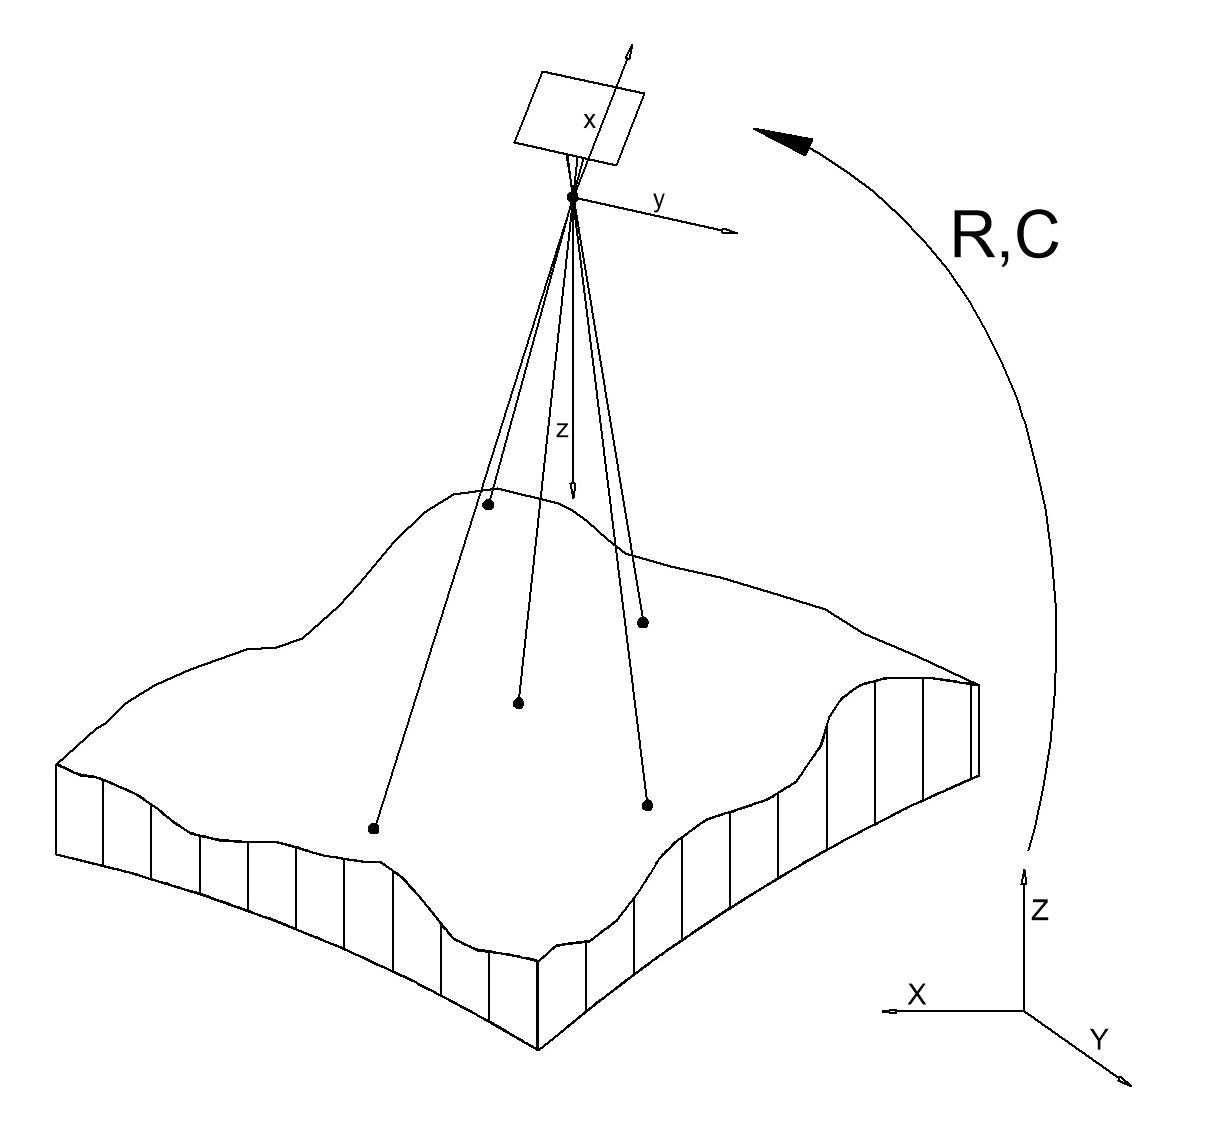
\includegraphics[scale=0.3]{figures/cv_object.png}
    \caption{Computer vision camera coordinate system in arbitrary object coordinate system.}
    \label{fig:cv_model}
\end{figure}

The equation can be abbreviated as:

\begin{equation}
\label{eq:p_exp}
\ehvect{x} = \ematr{K} \ematr{[}\ematr{R}|\evect{t}\ematr{]} \ehvect{X}
\end{equation}

\noindent where:

\begin{itemize}
\item \ematr{K} is calibration matrix which contains interior orientation parameters,
\item \ematr{[\ematr{R}|\evect{t}]} matrix contains rotation matrix \ematr{R} and vector $\evect{t}$.
	      They transform a point from the object coordinate system 
	      to the camera coordinate system. 
	      The vector $\evect{t}$ can  be transformed by:
	      \begin{equation}
	      \ehvect{C} = - \ematr{R}^{T}\evect{t}
	      \end{equation}
	      giving coordinates of camera projective center in object space. 
	      The rotation matrix \ematr{R} and the projective 
	      center object coordinates $\evect{C}$
	      represent exterior orientation of the camera.   
\item $\ehvect{X}$  homogeneous coordinates of an object point,
\item $\ehvect{x}$  homogeneous coordinates of transformed photo point.
\end{itemize}

Whole projection can be merged into single matrix \ematr{P} called camera matrix:

\begin{equation}
\label{eq:p_abbr}
\ehvect{x} =  \ematr{P} \ehvect{X} = \ematr{K} \ematr{[}\ematr{R}|\evect{t}\ematr{]} \ehvect{X}
\end{equation}

\subsubsection{Two photos geometry}
\label{sec:epipolar_gem}
%%% ML: prvni veta odstavce zni divne
%%% ST:prepsano

%%% ML: na konci vety by mela byt reference na obrazek
%%% ST: snad o neco lepsi

%%% -> ML: OK

%%% -> ML: osobne bych prvni vetu uplne vynechal
%%% -> ST: done

%In this chapter, there is mathematically derived relation of two photos.
The core of the two photos geometry arises from epipolar geometry.
The relation describes transformation from a photo coordinate system of the \term{first photo} to 
a photo coordinate system of the \term{second photo} and vice versa.

%%% ML: prvni veta zni taky divne 

%%% -> ML: OK

If the same object point is identified on both photos,  
epipolar plane $\pi$ goes through the photo points and the object point. 

\begin{figure}[h]
    \centering
    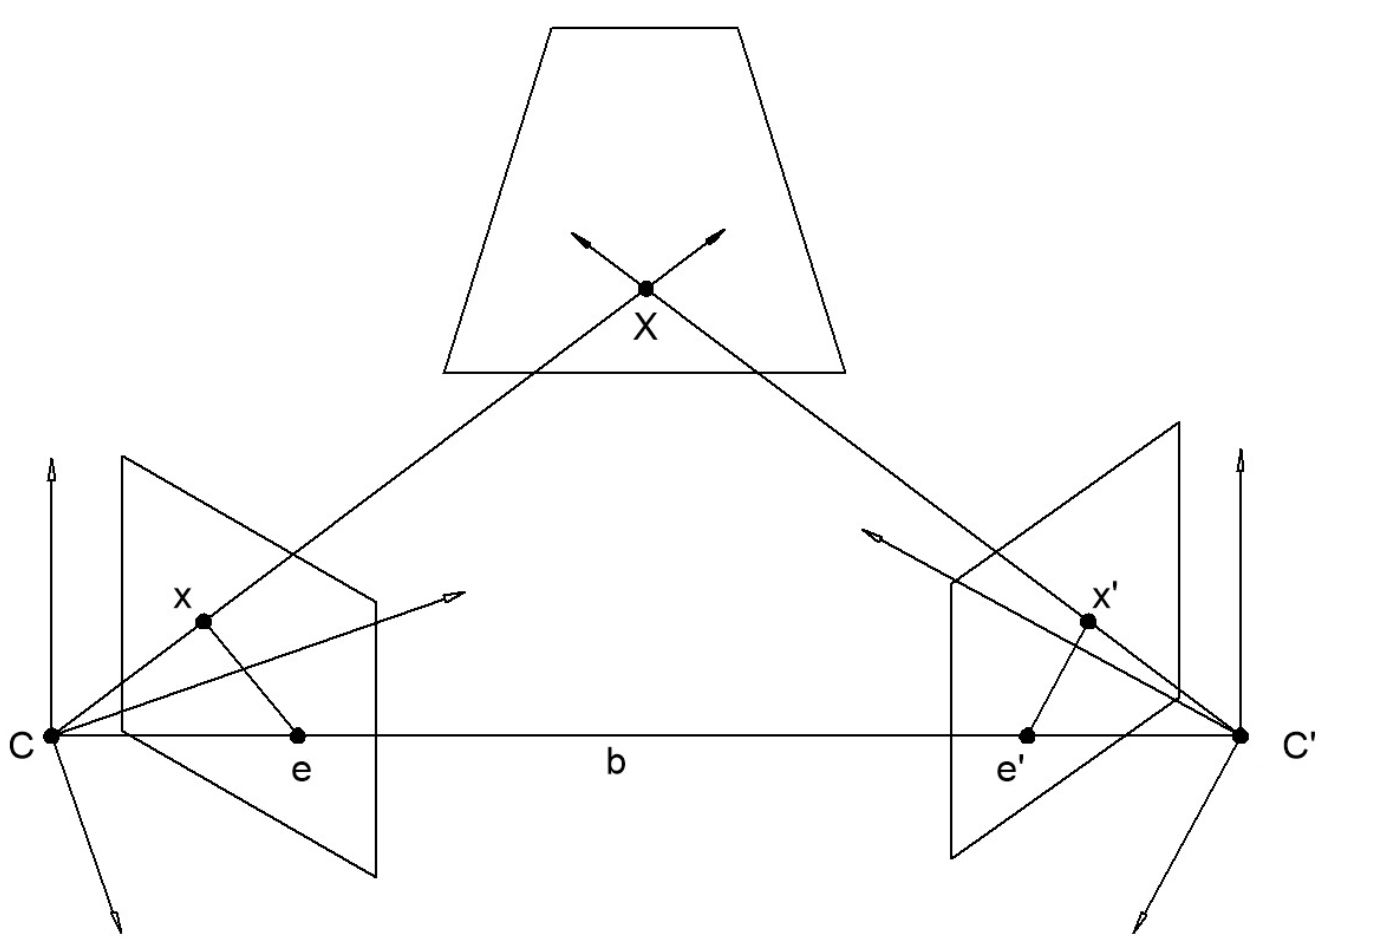
\includegraphics[scale=0.3]{figures/epipolar.png}
    \caption{Epipolar geometry.}
    \label{fig:epipolae}
\end{figure}

An epipolar plane contains following elements:

%%% ML: v textu pouzivas dva styly - prvni zacina velkym pismenem a
%%% teckou; druhy malym pismenem (nekdy konci carkou nebo bez carky),
%%% osobne bych se priklanel zacinat malym pismenem a koncit carkou,
%%% posledni potom konci teckou, chtelo by to sjednotit (low
%%% priority), podstatne je zachovat jednotny styl, jinak to zbytecne
%%% rusi
%%% ST: styl sjednocen

\begin{itemize}
\item two rays connecting object point with photo points and camera centers of both photos,
\item baseline \escal{b} connecting projection centers (\evect{C}, \evect{C'}) of the photos,
\item epipoles (\escal{e}, \escal{e'}) lying on an intersection of a photo plane with a baseline,
\item epipolar lines  $(\escal{l}_{e}, \escal{l'}_{e})$ going through epipole and photo point. It belongs into a photo plane.
\end{itemize}

%%% ML: "which comes form epipolar geomatry" -> "which comes from
%%% epipolar geometry", ale i tak zni divne
%%% ST:prepsano

\noindent Following relations arise from epipolar geometry:
\begin{itemize}
\item All epipolar lines of  photo intersect in a epipole. If the photos are merely translate with no difference in orientation, 
 epipoles lie in infinity.
\item A photo point forms epipolar line in the other photo. It allows to reduce space of possible occurrence of the point 
      from \eucl{2} to \eucl{1} of epipolar line without some other information about the point e.g. object space coordinates. 
\end{itemize}

%%% ML: projection? first photo system? - to bude tou pozdni hodinou ;-)

%%% ML: Reverse the transformation, bez "the", rectangular shape (3 x 4) ???
%%% ST: prepsano

Camera matrix \ematr{P} \eqref{eq:p_abbr} represents projective transformation from object system to the first photo system.
Reversed transformation can not be done by inverse matrix because of the rectangular shape (3x4) of 
camera matrix \ematr{P}. Instead of matrix inversion,  pseudo inverse matrix $\ematr{P}^{+}$ must be 
calculated to reverse the transformation. Pseudo inverse matrix has this property: $\ematr{P}\ematr{P}^{+} = \ematr{I}$.
Singularity of the matrix can be interpreted as consequence of information loss caused 
by dimensional reduction done by transformation of 3D object point into 2D photo plane.  

A point $\ehvect{x}$ of the  first photo system  
can be transformed into  
 the second photo system as point $\ehvect{x'}$
by:

\begin{equation}
\ehvect{x'} =  \ematr{P'}\ematr{P}^{+}\ehvect{x}
\end{equation}

where \ematr{P} and \ematr{P'} are camera matrices of the first and the second photo.
%%% ML: "One variant, how a line can be defined, is by direction and
%%% point." divne receno, TODO for me: projit tuto kapitolu jeste jednou...
%%% ST:prepsano

The transformed point $\ehvect{x'}$ lies at infinity 
representing direction of a epipolar line $\escal{l'}_{e}$. A line can be define by a direction 
and a point. In order to define epipolar line $\escal{l'}_{e}$ missing point can be obtained from 
projection of the first camera projective center $\evect{C}$ into the second photo system where it represent
epipole:

\begin{equation}
\ehvect{e'} =  \ematr{P'}\ehvect{C} \\
\end{equation}


%According to  \eqref{eq:hline} line can be given as:

%\begin{equation}
%\ematr{X}(\escal{\lambda}) = \ematr{P}^{+}\ehvect{x} + \escal{\lambda}\ehvect{C}
%\end{equation}

%%% ML: using?
%%% ML: prepsano

Epipolar line is given \eqref{eq:def_hline_pts} by:

\begin{equation}
\ehvect{l'_{e}} =  \ehvect{e'} \times \ehvect{x'} = (\ematr{P'}\ehvect{C}) \times \ematr{P'}\ematr{P}^{+}\ehvect{x}
\end{equation}

Cross product of two vectors \evect{a} and \evect{b} can be also written as multiplication of a matrix and a vector:

\begin{equation}
\evect{a}  \times \evect{b}  = 
\begin{pmatrix}
   & 0      & \escal{a_{3}}   & \escal{a_{2}}\\
   & \escal{a_{3}}  & 0               & \escal{-a_{1}}\\
   & \escal{-a_{2}} & \escal{a_{1}}   & 0\\
\end{pmatrix}
\evect{b} = [a]_{\times} b
\end{equation}

%%% ML: Using ... gives (to nezni moc anglicky)
%%% ST: prepsano
The epipolar line equation can be rewritten using the matrix notation of cross product as:
\begin{equation}
\ehvect{l'_{e}}  = [\ehvect{e}']_{\times} \ematr{P'}\ematr{P}^{+}\ehvect{x}
\end{equation}

%%% ML: tento odstavec by chtel prepsat...
%%% ST: prepsano

It is apparent from the equation that matrix denoting relation of two photos is defined as:

\begin{equation}
\ematr{F}  = [\ehvect{e}']_{\times} \ematr{P'}\ematr{P}^{+}
\end{equation}

Matrix \ematr{F} is called a \term{fundamental matrix} \cite{Hartley2004}. 
It transforms photo points of the first photo system into 
epipolar lines of the second photo.
Fundamental matrix can be expanded by \eqref{eq:p_abbr}
allows to derive another important matrix of two view geometry called \term{fessential matrix} \ematr{E}.

%%% ML: zvyraznit "fundamental matrix" (?)
%%% ST: zvyrazneno

Lets suppose that camera matrix of the first photo is defined in this way:
\begin{equation}
\ematr{P}  = \ematr{K} \ematr{[}I|0\ematr{]}
\end{equation}
It means that the first camera coordinate system coincides with  the object space coordinate 
system.

Its pseudo inverse matrix is:
\begin{equation}
\label{eq:rel_or_inv_cam1}
\ematr{P}^{+} =
\begin{pmatrix}
   \ematr{K}^{-1} \\
   \evect{0^{T}} \\
\end{pmatrix}
\end{equation}

Homogeneous object projective center coordinates are:
\begin{equation}
\label{eq:c1}
\ehvect{C} =
\begin{pmatrix}
   \evect{0} \\
    1 \\
\end{pmatrix}
\end{equation}

The second camera matrix is defined in this way:
\begin{equation}
\label{eq:rel_or_cam2}
\ematr{P}'  = \ematr{K}' \ematr{[}\ematr{R}|\evect{t}\ematr{]}
\end{equation}


Epipole of the second photo is given as:
\begin{equation}
\begin{split}
\label{eg:second_epipole}
\ehvect{e'} &=  \ematr{P'}
\begin{pmatrix}
   \evect{0} \\
    1 \\
\end{pmatrix} \\
&= \ematr{K}' \evect{t}\\
\end{split}
\end{equation}

The relationship of two cameras is also called \term{relative orientation}, because rotation matrix \ematr{R} and vector \evect{t}
represents orientation and position of the second camera to the first one. This relationship is defined up to scale.
In order to express cameras exterior orientations in a world coordinate 
system or merge it with another relative orientations, it is needed to perform further transformations of the relative 
exterior orientations, for more information see chapters \ref{sec:ess_chain} and \ref{sec:helmert}.

The fundamental matrix equation can be rewritten taking into account the relative orientation \eqref{eq:rel_or_inv_cam1},
\eqref{eq:rel_or_inv_cam1} and \eqref{eq:c1}  as:

\begin{equation}
\label{eg:funeq}
\begin{split}
\ematr{F}  &= [\ematr{P}'\ehvect{C}]_{\times} \ematr{P}'\ematr{P}^{+}
= [\ematr{K}' [\ematr{R}|\evect{t}]
\begin{pmatrix}
   \evect{0} \\
    1 \\
\end{pmatrix}]
_{\times} 
\ematr{K}' [\ematr{R}|\evect{t}]  
\begin{pmatrix}
   \evect{K}^{-1} \\
   \evect{0}^{T} \\
\end{pmatrix} \\
&= [\ematr{K}' \evect{t}]_{\times} \ematr{K}'\ematr{R}\ematr{K}^{-1} \\
&= [\ehvect{e}']_{\times} \ematr{K}'\ematr{R}\ematr{K}^{-1} 
\end{split}
\end{equation}

Now there comes little bit more difficult part.
This formula applies for any non-singular matrix \ematr{M} and vector \evect{x} \cite[p. 582]{Hartley2004}:
\begin{equation}
\label{eg:furmula}
[\evect{x}]_{\times} \ematr{M} = \ematr{M}^{-T}[\ematr{M}^{-1}\evect{x}]_{\times}
\end{equation}

The fundamental matrix equation can be further rewritten using the formulas \eqref{eg:furmula} and \eqref{eg:second_epipole}:  
\begin{equation}
\begin{split}
\ematr{F}  &= [\ehvect{e}']_{\times} \ematr{K}' \ematr{R} \ematr{K}^{-1} \\
	  &= \ematr{K}'^{-T} [\ematr{K}'^{-1} \ehvect{e}']_{\times} \ematr{R} \ematr{K}^{-1} \\
	   &= \ematr{K}'^{-T} [\ematr{K}'^{-1} \ematr{K}' \evect{t}]_{\times} \ematr{R} \ematr{K}^{-1} \\
	   &= \ematr{K}'^{-T} [\evect{t}]_{\times} \ematr{R} \ematr{K}^{-1}
\end{split}
\end{equation}

This equation reveals very important fact about fundamental matrix saying that a transformation performed 
by matrix can be divided into three main steps.

In first step, photo coordinates of point are normalized.
Normalized coordinates of the first photo are transformed 
into normalized coordinates of the second photo by essential matrix:

\begin{equation}
	 \ematr{E}  = [\evect{t}]_{\times} \ematr{R}
\end{equation}

Eventually, the coordinates are transformed into photo system of the second photo
representing epipolar line.     

It follows that the essential matrix incorporates a relative orientation of two photos.
Essential matrix is subset of whole information encoded in fundamental matrix.
Fundamental matrix includes
additional information about interior orientations of cameras which took the photos.  

Hence, if exterior orientation of a two photos is known, the
essential matrix can be computed. The matrix can be calculated from exterior orientations 
independently of specific object coordinates system since it takes into account the relative 
position of two photos up to scale. Moreover, if calibration matrices 
are know, it is possible to define relationship (without taking into account distortion) between 
 the two photo systems by fundamental matrix.

\subsubsection{Triangulation of points}
\label{sec:triang}

Triangulation methods deal with retrieval of the object point coordinates
from corresponding points in photos. 
If measurements would be precise, object point 
would lie on intersection of two rays which is clearly visible on 
 Figure \ref{fig:obj_intersec}. Unfortunately the rays are never determined so precisely to intersect.
 Several methods deals with the imperfections.

Direct linear transformation (DLT) method  is based 
on linearization of collinearity equations \eqref{eq:col_eqs}
employing least square method on it.

The simplified DLT collinearity equations can be written as \cite{pavelka2004foto10}[p. 130]:  
\begin{equation}
\begin{split}
&\escal{x}^{un} = \frac{\escal{a}_{1}(\evect{X}^{obj}) + 
                                  \escal{a}_{2}(\evect{Y}^{obj}) + 
                                  \escal{a}_{3}(\evect{Z}^{obj}) +
                                  \escal{a}_{4}
                                  }{
				  \escal{a}_{9}(\evect{X}^{obj}) + 
                                  \escal{a}_{10}(\evect{Y}^{obj}) + 
                                  \escal{a}_{11}(\evect{Z}^{obj}) +
                                   1  
                                  } \\
&\escal{y}^{un} = \frac{\escal{a}_{5}(\evect{X}^{obj}) + 
                                  \escal{a}_{6}(\evect{Y}^{obj}) + 
                                  \escal{a}_{7}(\evect{Z}^{obj}) +                                 
                                  \escal{a}_{8}
                                  }{
				  \escal{a}_{9}(\evect{X}^{obj}) + 
                                  \escal{a}_{10}(\evect{Y}^{obj}) + 
                                  \escal{a}_{11}(\evect{Z}^{obj}) +    
                                  1
                                  }
\end{split}
\end{equation}
 
It can be expressed in linear form:

\begin{equation}
\begin{split}
\escal{x}^{ph} =& \escal{a}_{1}\evect{X}^{obj} + 
                                  \escal{a}_{2}\evect{Y}^{obj} + 
                                  \escal{a}_{3}\evect{Z}^{obj} +
                                  \escal{a}_{4} \\
				  &- \escal{x}^{ph} \escal{a}_{9}\evect{X}^{obj} -
                                  \escal{x}^{ph} \escal{a}_{10}\evect{Y}^{obj} - 
                                  \escal{x}^{ph} \escal{a}_{11}\evect{Z}^{obj} \\
\escal{y}^{ph} =& \escal{a}_{5}\evect{X}^{obj} + 
                                  \escal{a}_{6}\evect{Y}^{obj} + 
                                  \escal{a}_{7}\evect{Z}^{obj} +                                 
                                  \escal{a}_{8}\\
				  &- \escal{y}^{ph} \escal{a}_{9}\evect{X}^{obj} -
                                  \escal{y}^{ph} \escal{a}_{10}\evect{Y}^{obj} - 
                                  \escal{y}^{ph} \escal{a}_{11}\evect{Z}^{obj}    
\end{split}
\end{equation}
 
%%% ML: prvni veta zni divne, min. chybi "implement *it*"

Because of linearity, it does not require to know approximate values. 
Main drawback of this method is that DLT model does not respect pinhole camera model thus
minimized parameters in the vector \evect{a} do not follow rigorous camera geometry which 
may result in inaccurate retrieval of object coordinates. Another problem of the method 
is that it is not fully linear because variables $\escal{x}^{ph}$ and $\escal{y}^{ph}$
occurs also in the right side of the equations. 

%%% ML: chtelo by zvyraznit "optimal solution"

More complicated method is called the \term{optimal solution}. 
It is based on enforcing epipolar constraint.  The cost function 
minimizes sum of squares of distances between photo points to epipolar lines created 
by transformation of corresponding photo points from another photos.

The cost function is not linear, however, it's derivative leads into 6 degree polynomial thus 
it has 6 roots. Correct solution can be selected from roots by assumption that it represents global minimum. 

This method is considered by computer vision community as the most accurate \cite[p. 315]{Hartley2004}.  

\subsubsection{Retrieving of relative orientation from essential matrix}
\label{sec:ess_eo}

%%% ML: Rotation *matrix* ? (opraveno, dal v textu pouzivas)

%%% ML: Singular Values Decom. (velkymi pismeny?)
%%% ST: malymi viz. http://en.wikipedia.org/wiki/Singular_value_decomposition

Rotation matrix \ematr{R} and vector \evect{t} can be retrieved from the essential matrix using 
singular values decomposition (SVD):

%%% ML: tahle rovnice vypada divne...
%%% ST: snad lepsi 

\begin{equation}
\begin{split}
\ematr{W} &=
\begin{pmatrix}
& 0 & -1 & 0 \\
& 1 & 0 & 0 \\
& 0 & 0 & 1\\
\end{pmatrix} \\
 \ematr{R} &= \ematr{U}  \ematr{W} \ematr{V}^{T}\\
 \evect{t} &= \evect{U}_{3,:}
\end{split}
\end{equation}

where matrices \ematr{U} and \ematr{V} are two rotation matrices  obtained for SVD decomposition.
The retrieved rotation \ematr{R} matrix and the shift vector \evect{t} are defined up to sign,
which causes four case ambiguity. 

As a consequence of the  ambiguity it gives four relative orientations: 
\begin{equation}
[\ematr{R}|\evect{t}],
[\ematr{R}|\evect{-t}],
[\ematr{-R}|\evect{t}],
[\ematr{-R}|\evect{-t}],
\end{equation}


The correct solution can be found   by assumption that all object points has to be in the front
of the both photo planes.

\begin{figure}[h]
    \centering
    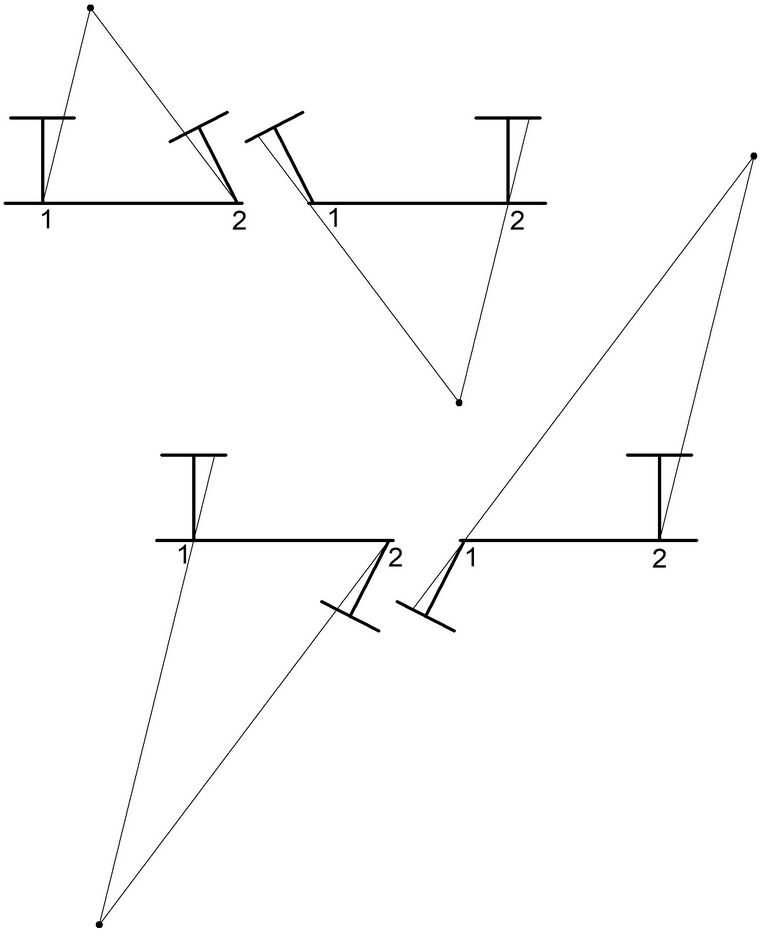
\includegraphics[scale=0.25]{figures/eo_ambiguity.png}
    \caption{Four possible relative orientations of photos (1, 2) retrieved from an essential matrix.
    Note that only the upper left configuration satisfies condition that object point 
    must be in front of both photo planes. (Based on \cite[p. 19]{pietzsch2001robot})}
    \label{fig:rel_or_amb}
\end{figure}


\subsubsection{Merging relative orientations}
\label{sec:ess_chain}

%%% ML: posledni veta odstavce potrebuje korekce

If two relative orientations are merged together, they must share one photo.
As a first step, it is necessary to calculate a scale \cite{pietzsch2001robot}
because relative orientation coordinate systems are independent of scale.
The scale can be calculated from corresponding distances measurable in  both coordinate systems. 
Distances between object point determined in both camera systems and object coordinates of projective center of shared photo 
can be used for calculation of scale:

\begin{equation}
\escal{s}^{ro2-1} = \frac{||\mathbf{\evect{X}^{ro1}_{1} - \evect{C^{ro1}_{1}}}||}
	                {||\mathbf{\evect{X}^{ro2}_{1} - \evect{C^{ro2}_{1}}}||}
\end{equation}

Where:
\begin{itemize}
\item \term{ro1}, \term{ro2} are relative orientation coordinate systems. 
System \term{ro2} is transformed into system \term{ro1}. 
\item \evect{X} is an object point determined in both relative orientations,
\item \evect{C} is a projective center of the shared photo.
\end{itemize}

\begin{figure}[h]
    \centering
    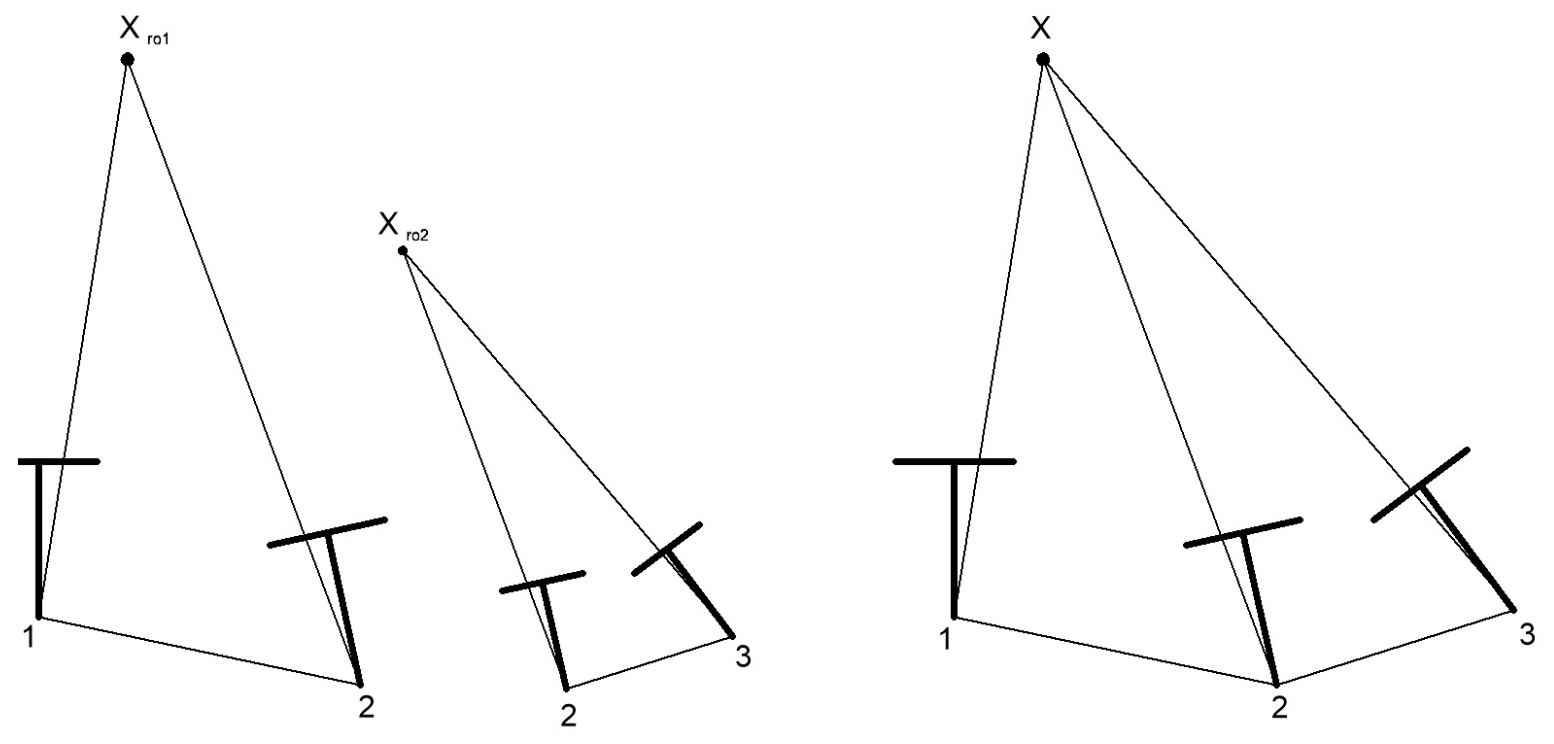
\includegraphics[scale=0.25]{figures/rel_or.png}
    \caption{In the left picture there are relative orientations \term{ro1}, \term{ro2} before transformation 
    to a common system. 
    In the right picture, there is common system defined by \term{ro1} after transformation of \term{ro2}. 
    Note change of \term{ro2} scale after the transformation. (Based on \cite[p. 20]{pietzsch2001robot})}
    \label{fig:rel_or_amb}
\end{figure}

%%% ML: "coincides to" ?
%%% ST: vynechano

%%% ML: Usually ?
%%% ST: jj

Usually bundles of photos capturing a scene are processed. Photo pairs comprising relative orientation capture only fragments of a scene, 
therefore the information of scene is scattered.  
In order to interpret the scene as whole it is needed to merge all relative orientation systems into \term{common relative coordinate system}.
For sake of simplicity, the common relative system is defined by relative orientation system of arbitrary pair called \term{reference pair}.
Other relative orientations are subsequently transformed into the common coordinate system. 

%%% ML: transformed into?
%%% ST: prepsano

All relative orientations which can be transformed into common system are
 connected component of undirected graph.  Nodes represents  photos and edges denotes relative orientations. 
In other words, it is possible to transform relative orientation into the common relative coordinate system only, if there 
is a continuous chain of the relative orientations from reference pair 
to the transformed orientation, where every two neighborhood relative orientations in the chain share one photo.

The transformation of relative orientations 1-$n$ into common system defined by relative orientation 1 can be written as: 
\begin{equation}
\label{eq:comm_rel}
\begin{split}
&\ematr{P}_{1\_co} = [\ematr{I}|\evect{O}] \\
&\ematr{P}_{2\_co} = [\ematr{R}^{ro1}|\evect{t}^{ro1}] = [\ematr{R}^{ro1\_co}|\evect{t}^{ro1\_co}] \\
&\ematr{P}_{3\_co} = [\ematr{R}^{ro2} \ematr{R}^{ro1\_co}|\ematr{R}^{ro2} \evect{t}^{ro1\_co} + \escal{s}^{ro2-1} \evect{t}^{ro2}] 
=  [\ematr{R}^{ro3\_co} | \evect{t}^{ro3\_co}] \\
&\ematr{P}_{n\_co} = [\ematr{R}^{ro(n)} \ematr{R}^{ro(n)(n-1)\_co}|\ematr{R}^{ro(n)} \evect{t}^{ro(n-1)\_co} + \escal{s}^{ro(n)-(n-1)} \evect{t}^{ro(n)}] 
=  [\ematr{R}^{ro(n)\_co} | \evect{t}^{ro(n)\_co}] 
\end{split}
\end{equation}

The equations suppose that projection matrices in \escal{ro(n)} relative orientation system
are defined as $\ematr{P}_{n-1} = [\ematr{I}|\evect{O}]$ and $\ematr{P}_{n} = [\ematr{R}^{ro(n)}|\evect{t}^{ro(n)}]$.

\subsubsection{Helmert transformation}
\label{sec:helmert}

Helmert transformation can be written by equation:
\begin{equation}
\ematr{X}_{t} = \evect{t} + \escal{s}\ematr{R}\evect{X} \\
\end{equation}


where \ematr{R} is a rotation matrix, \escal{s} is a scale scalar, \evect{t} is a translation vector and
 $\evect{X}$ is transformed point into a point $\ematr{X}_{t}$.
The transformation is defined by seven parameters (three translation coordinates, three rotation angles and scale).
In order to get these parameters it is needed to know at least two corresponding points and  another one with 
at least one known coordinate in both coordinate systems. 

%%% ML: "There exists" zni divne
%%% ST: prepsano

Helmert transformation parameters can be retrieved from corresponding points by several methods.  
For instance closed form method can be employed based on SVD decomposition
\cite{sjoberg2013closed}.

\subsection{Bundle block adjustment}

Bundle block adjustment (BBA) is a method, which uses the least squares technique (\ref{sec:least}) to refine scene parameters. 
The main advantage of BBA is that the it takes into account whole scene and therefore it utilizes 
maximum information for adjustment of scene parameters which leads to the more accurate results.
The principle of BBA has been known for very long time since 1950s,
however, the method has been employed in practical applications since 1990's, because the performance of computers had not been 
sufficient enough before. 


\begin{figure}[h]
    \centering
    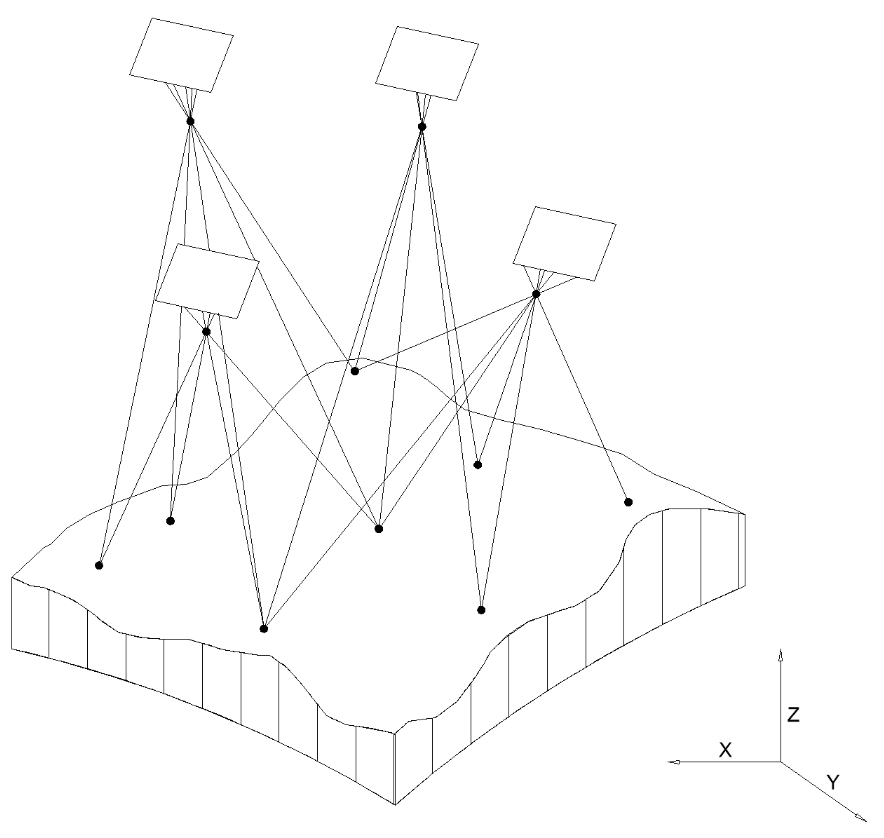
\includegraphics[scale=0.3]{figures/bba.png}
    \caption{BBA takes into account scene as whole.}
    \label{fig:rel_or_amb}
\end{figure}

The cost functions of BBA least squares method are photogrammetric collinearity equations \eqref{eq:col_eqs}.
The least squares method tries to find vector of adjusted parameters \evect{X} to minimize
sum  of square differences between coordinates of measured photo points and photo points calculated 
from collinearity equations.

Unfortunately, collinearity equations are non linear hence the non-linear least square method \ref{sec:non_least} must be employed, which 
needs to be provided  with sufficiently accurate initial values in order to find values of parameters satisfying minimization criterion.

Thanks to the least squares method, BBA is very flexible in terms of selection of the parameters to be adjusted. 
It is possible to select various combinations of interior, exterior orientations and object points coordinates parameters. 

Following example describes BBA in practice.
Lets suppose that initial values of adjusted parameters are known with sufficient accuracy in order to the least squares
method eventually iterate to global minimum.
Lets say that there is a scene captured by three photos.
All the photos were taken by same camera.
The cameras interior orientation is known accurately therefore it is not adjusted in BBA.
There are identified three tie points and two ground control points in all three photos.
Tie point is identified only in photos with missing information about its object coordinates.  
Unlike tie point, object coordinates of ground control point (GCP) are known.
Additional two tie points and one GCP are identified in two photos.
Also another one GCP and one tie point are identified 
in only one photo. 

%Initial values of tie point object coordiantes were obtained, but the values needed to be refined by BBA to improve its accuracy.

Every tie point needs to refine three parameters (object coordinates). 
Object coordinates of GCPs are known with high accuracy therefore they are not refined by BBA. 
If a point is identified on a photo, it yields two measurements (x, y collinearity equations) 
therefore it is needed to identify a tie point at least on two photos to get more measurements 
than unknowns. This makes perfectly sense because it is not possible to determine object point coordinates from one photo,
since it can lie wherever on the ray (see Figure \ref{fig:obj_intersec}).

Unlike tie points, GCPs do not bring any new adjusted parameters 
allowing to use the GCP visible only in single photo. In this case, the object coordinates 
are known thus there is no ray ambiguity. 

Lets suppose that it is adjusted exterior orientations and object coordinates of tie points.  
Every photo yields six parameters of exterior orientation (three projective center coordinates and three orientation angles) 
 giving 6 $\times$ 3 = 18 parameters. 

Tie points give 5 $\times$ 3 = 15 adjusted parameters of the object coordinates. 
Only 5 tie points are used in BBA because the tie point visible in just one photo must be skipped.
GCPs do not give any adjusted parameters since coordinates are known.

Every tie point and GCP visible on three photos give 6 measurements (two collinearity equations for every photo point)
totally giving 30 measurement.
Points visible from two photos give 4 measurements totally yielding 12 measurements.
GCP visible from single photo gives additional 2 measurements.

Overall score is 33 adjusted parameters and 44 measurements.

Thanks to 9 redundant measurements it is possible to add some of the interior parameters into adjustment.  
On the other hand the redundancy of measurement improves accuracy of results which is the main point of the least square method
therefore it should be avoided to have nearly same number of measurements and adjusted parameters.

%%% ML: TODO
%%% ST DONE

\begin{figure}[h]
    %\centering
    \hspace*{-1.0in}
   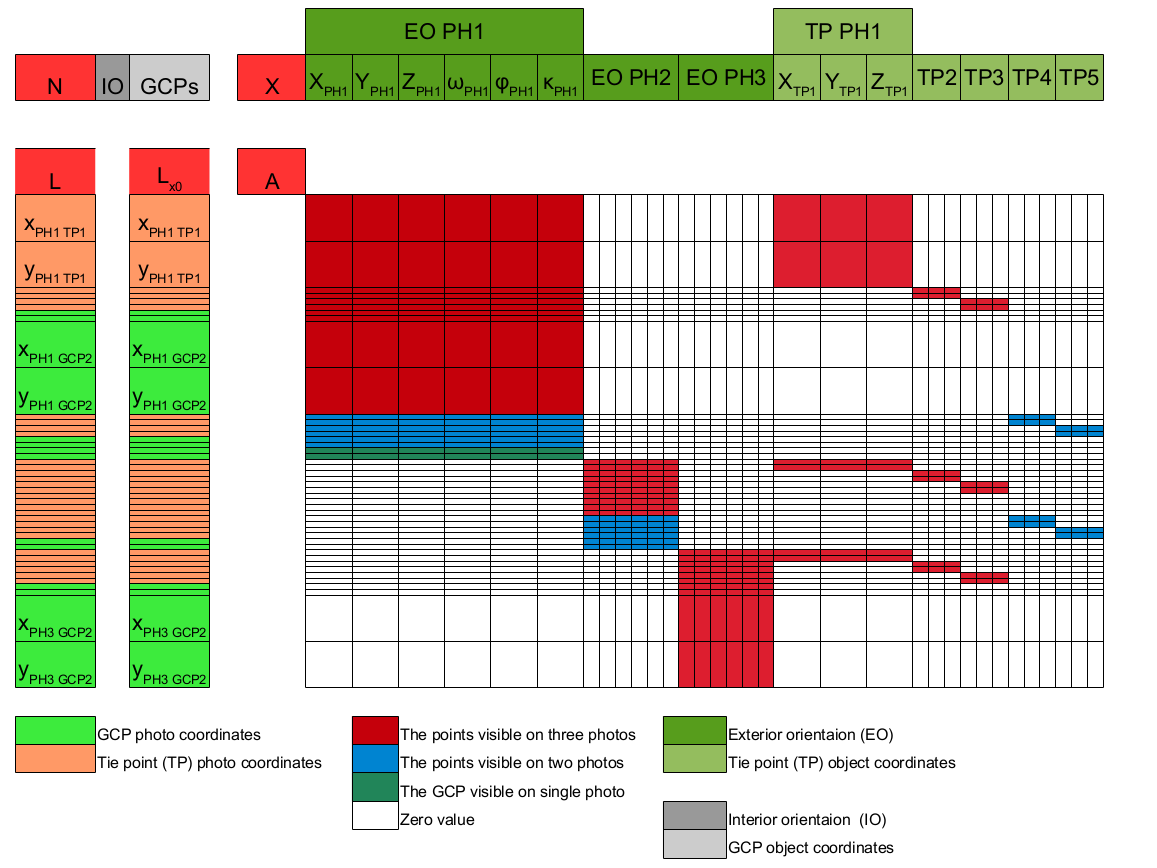
\includegraphics[scale=0.47]{figures/bba_system.png}
    \caption{Schematic picture of least squares elements of the example.}
    \label{fig:bba_system}
\end{figure}



In the first least squares iteration, the initial values of adjusted parameters are put into parameters vector $\evect{X}$
 representing tangent point of Taylor polynomial to costs functions.  The other non-adjusted 
parameters are given into $\evect{N}$ vector of knowns. In the example, non-adjusted parameters are object coordinates
of GCPs and interior orientation. 
Measured photo coordinates are given
into vector of measurements $\evect{L}$.

Design matrix $\evect{A}$ is calculated from 
derivatives of collinearity equations substituting values from vectors $\evect{X}$ and $\evect{N}$.

The vectors  $\evect{L}$ and  $\evect{X}$ give structure to design matrix $\evect{A}$ and
vector of $\evect{L}_{X0}$.
Order of partial derivatives of design matrix $\evect{A}$  is determined by adjusted parameters position in 
parameters vector $\evect{X}$. E.g. the first column of the example design matrix is filled with derivatives respect 
to variable representing the  X object coordinate of the first photo projective center. Variables of derived collinearity equations
depends on row. For instance, the first two rows represents partial derivative of collinearity functions 
including variables of the first point object coordinates  and first photo exterior orientation.  First row represents  
derivation of x collinearity equation because in corresponding position of the measurements vector $\evect{L}$, there is 
x photo coordinate of the tie point 1. The second row of the design matrix is composed of 
partial derivatives of y equation comprised of the same variables. 
Variables of collinearity equation change in the other rows. For instance, the last row corresponds to the 
y photo coordinate of the GCP 2. The partial derivation of the first column is equal 
to zero because the variable X object coordinate of the first photo projective center was replaced 
by X of the third photo projective center in collinearity equation. Also it should be noted that in the last row, there is no derivation 
respect to point object coordinates because the row represents GCP. Object coordinates of GCPs do not 
belong to the adjusted parameters thus design matrix do not contain column representing partial 
derivatives respect to the GCP object coordinates.

Position in a vector $\evect{L}_{X0}$ is connected in the same way to a vector $\evect{L}$ as rows of design matrix.
Value of position is calculated by collinearity equations using corresponding variables.

The relations nicely illustrates a pivot role of design matrix which links parameters vector $\evect{X}$ 
with measurements vectors $\evect{L}$ and $\evect{L}_{X0}$.

If rows in design matrix $\evect{A}$ or positions $\evect{L}$ and $\evect{L}_{X0}$ are switched,
as consequence of the correspondence it is needed to switched them also in the other components. 
Same applies for columns  of design matrix $\evect{A}$  and positions in parameters vector $\evect{X}$

All needed information is available to perform a first iteration of non linear least square 
method \ref{sec:non_least}. As result of iteration refined values of vector  $\evect{X}$
are obtained. Another iteration can be  performed by same procedure  with adjusted parameters vector $\evect{X}$
if termination criterion is not meet \ref{sec:term_crit}.

\subsection{Orthorectification}
\label{sec:ortho}

%%% ML: "same density" - spise rovnomerna, pravidelna
%%% ST: opraveno uniform
Orthorectification is a process transforming photo from perspective projection into orthogonal projection (see Figure \ref{fig:ortho}). 
There are two main methods for producing orthophoto. The first method is able to retrieve orthophoto 
from single photo. It requires exterior, interior orientations of the photo and a shape of relief. 
Shape of relief is usually provided in a form of digital terrain model (DTM). DTM 
can be given in the raster or vector form. Raster-based DTM describes relief with a uniform density defined 
by resolution of the raster.
Vector-based DTM is comprised by continuous surface made of triangular irregular network (TIN). 
At the beginning of orthorectification, empty raster is allocated representing an orthophoto.
It covers intersection of a photo scene and area of a DTM.

In the next step, empty orthophoto is filled by values. 
All points representing centers of pixels are given Z coordinates from DTM 
then the points are transformed into the photo coordinate system using collinearity equations.
Because a transformed point is represented by floating point, value given 
to the corresponding pixel in an orthophoto is determined by interpolation of surrounding pixels of the transformed 
point into a photo.  Used interpolation methods, selection of points 
for transformation etc. may vary, however, 
 the main principle is still the same. It is based on back projection of  an object point into 
a photo to obtain values for an orthophoto.

%%% ML: fix broken \ref{sec:triang}
%%% ST: fixed

The other method can be considered an extension of the first one because initially it generates DTM then it recovers orthophoto 
according to the same principle as the first method. It is based on triangulation of object point
from photo points requiring interior and exterior orientation of photos to be known. The reconstructed point 
must be visible at least on two photos in order to solve the ray ambiguity. It follows that it requires more than 
one photo in contrast to the first method.
Object coordinate system 
can be defined arbitrarily because there is no needed to define relationship to input DTM as the first method requires.
Instead of this, DTM is created in arbitrary coordinate system directly by the method,
hence orthophoto and DTM can be generated without any GCP. 
Approximate object points  are calculated by triangulation 
methods \ref{sec:triang} then refined by the BBA. 

The DTM is created from retrieved object coordinates. There 
are plenty of methods for DTM creation from points. Raster DTM can be created by various interpolation methods 
predicting value of raster according to surrounding points. Commonly used method for  creation of 
vector DTM (TIN) is Delaunay triangulation creating surface comprised of triangle network whose corners are located 
on object points. The triangulation finds such a configuration of triangles that no object 
point is inside the circumcircle of any triangle.
If big number of points are processed, finite element method 
should be used instead of Delaunay triangulation because it is computationally more efficient.
Unlike Delaunay triangulation which creates surface including all object points, finite element method
is based on principle of dividing triangles into smaller ones. 
The triangle is split until it sufficiently approximates surrounding object points. 
This method is able to create DTM from millions of points.

\begin{figure}[h]
    \centering
    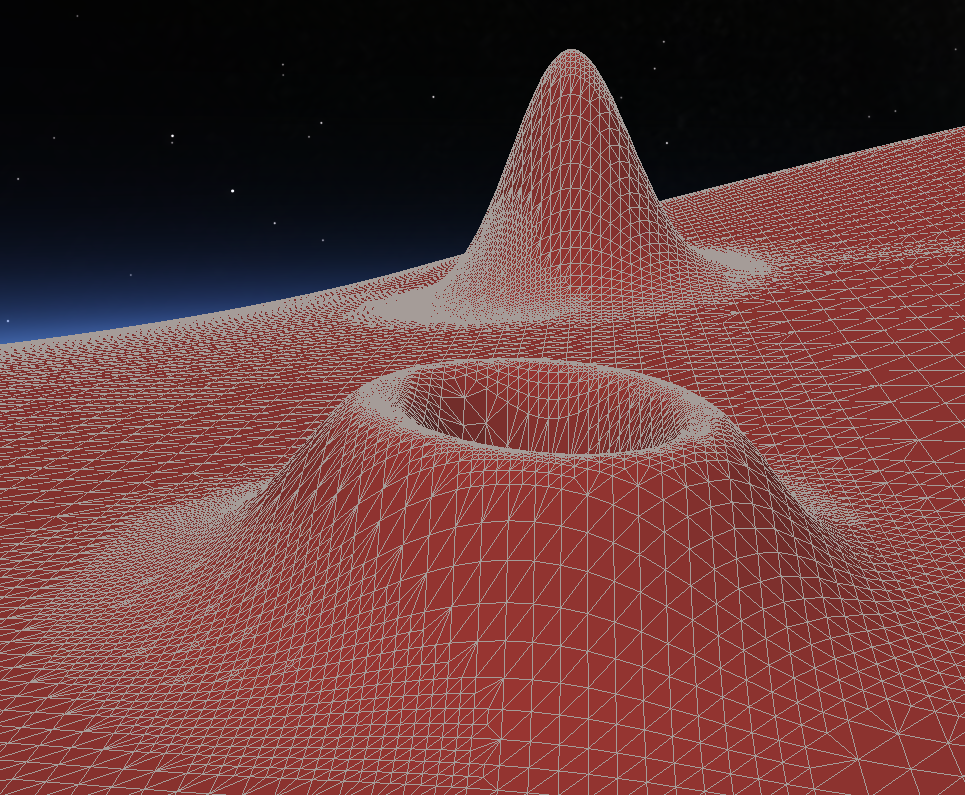
\includegraphics[scale=0.2]{figures/finite_elements.png}
    \caption{TIN created by Finite element method.}
    \label{fig:rel_or_amb}
\end{figure}

After obtaining of DTM, orthophoto can be created using same principle described in the first method. 

%%% ML: kapitola by mela zacinat na nove strane

\section{Analytical part}

\subsection{General solution of UAV bundle block adjustment}
\label{sec:solution}
%%% ML: "sattelite navigation" je hodne zkracene, spise bych uvedl GNSS
%%% ST: prepsano 

%%% ML: ZADNA REFERENCE V TEXTU ??? obecneji receno v textu je vubec
%%% malo referenci na literaturu, zkus to projit a nejake pridat

In 1990s Global Positioning System (GPS) become first globally operational navigation satellite system.
GPS allows 
to locate position of GPS unit with accuracy ranging  from  millimeters to decimeters depending 
on used technique and other conditions. 
In photogrammetry, GPS is often employed with inertial measurement unit (IMU), which measures its orientations in a object space.
The units greatly simplifies obtaining of initial values of exterior orientation in photogrammetric aerial mapping missions.
They provide all needed parameters of exterior orientation with sufficient accuracy for performing of BBA. 
In order to be information useful, it is need to determine 
lever-arm offset describing shift of GPS unit to the perspective center and bore sight offset
describing orientation of camera coordinate system towards IMU coordinate system \cite{perry2009synthesized}[p. 33]. These two
quantities are determined in calibration process \cite{perry2009synthesized}[p. 54]. The measured values from GPS and IMU units has to
be corrected by the two quantities to represent true exterior orientation of a camera coordinate system. The quantities
can be refined by BBA if collinearity equations are extended to include them.

\label{sec:assum}
Before operation of GPS, aerial photogrammetry had made some a priori assumptions about a camera position,
which simplified the collinearity equation in order to get initial values of exterior orientation. 
For instance, it can be assumed that the aerial photo is vertical if orientation deviates from true vertical
direction up to 2-3 degrees. Applying the assumption to collinearity equations, they can be linearized and 
approximate values can be computed easily from GCPs. \cite{pavelka2004foto20}[p. 52].
%%% ML: budget ... high - zni divne ...

Photogrammetric aerial mapping mission is prepared and carried out by experts using 
professional, properly calibrated equipment.
As a consequence, cost of the missions
is high. These facts prevents from further spreading of rigorous aerial photogrammetry methods.

Nowadays, nearly everybody has camera in his or her pocket thus there is a big demand 
to provide very simple solution from the user point of view because 
vast majority of the users have limited or no knowledge of photogrammetry and computer vision. 
 Recent rise of civil UAV \ref{sec:UAV_intro} sector has drastically reduced cost of mapping   
  compared to rigorous aerial photogrametry mission employing manned aircraft.

%%% ML: do textu bych vice zaclenil reference na teoritickou cast

It follows the main requirement 
of the solution to be simple and cheap enough
in order to be adopted by
ordinary users who do not want 
to spend money for other devices or spend time studying complicated methods. 
Ordinary users just 
want to take a group of a photos of a scene and get the job done by a software.
The final solution should be flexible to process both terrestrial and aerial photos
giving orthophoto and structure/DTM as an output. 
No limitation on camera orientation should be enforced because it should be capable 
of processing photos captured from camera held by hand or mounted on UAV.
Due to instability of UAV flight track and human hand, the photos 
must be considered as oblique. 

%%% ML: posledni veta: download -> share ?
%%% ST: ok

In order to meet the requirement of simplicity, user should just need  
 camera to obtain structure of the scene. Orthophoto creation would also need employment of UAV
in order to get images from approximately vertical point of view.
No other hardware device should be needed. 
All other steps should be done 
using free software, which can everybody freely share and use. 

%%% ML: v textu pouzivas velmi casto konstrukce s where/who/which

The solution should be flexible enough to process additional data known about a scene, 
e.g. GCPs, positions of cameras etc. The additional data can
 increase accuracy of results and reduce computational time  
 decreasing number of  BBA iterations needed for finding global minimum. It is very important 
 for professional photogrammetric measurements where accuracy matters.

As consequence of the general goals the minimum required input should be just photos
of the scene.
It could be required to take photos of a calibration scene, however, 
it must be easy to construct it. 

Another important requirement is to make whole process as much automatic as possible, 
because if it would require a lot of time for an user to go through the processing chain, nobody would use it.

Following processing chain  \cite{labe2006automatic} should fulfill above mentioned requirements for the solution:

\begin{itemize}
\item Camera calibration - determination of camera interior orientation.  One group of many techniques for calibration
of camera are based on processing of photos of 2D calibration patterns. Whole process is very simple from the user point of view. It is needed 
to print the pattern on sheet of paper and take photos of the pattern from different positions. The calibration 
is done automatically. No additional user input except a photos of a pattern is needed.
\item Tie point identification - it can be done fully automatically by pattern matching algorithms.
\item Retrieval of initial values for BBA - it is fully automatic process without need of any manual user input.
As input it needs tie points and interior orientation of camera given by previous two steps.
 Optional step of transformation into world coordinate system needs users assistance
 to provide GCPs \cite{heipke1997automation} in most cases.
\item Bundle block adjustment - it is fully automatic integrating information from all three previous steps.
\end{itemize}
 
\subsubsection{Camera calibration}
\label{sec:cam_calib}
%%% ML: druha veta by chtela prespat
%%% ST: vypustena 

Camera calibration is a process dealing with determination of the interior orientation parameters including distortion.
Several methods can be used for camera calibration \cite{zhang2004calibration}. 
%%% ML: one family zni divne
%%% ST: group
%%% ML: which *have* psal bych bez carky, i tak ta veta zni moc 'cesky' :-)
%%% ST: prepracovano
One group of calibration methods are based on photos capturing calibration object covered with calibration points.
Relative position of the points to each other is  precisely determined.  

The methods can be further divided according to dimension of a calibration object:

%%% ML: osobne bych zvyraznil jednotlive polozky ({\em })
%%% ML: zvyrazneno

\begin{itemize}
\item \term{3D reference object based calibration} -- It allows to reach very good accuracy of determined 
interior orientation parameters. One type of common calibration objects is comprised of three or two
perpendicular planes covered by calibration points. Drawback of 3D calibration 
is that accurate construction of the calibration object is difficult.
\item \term{2D plane based calibration} -- It is less accurate compared to 3D calibration. 
The accuracy can be improved by taking more photos of a calibration object.
On the other hand calibration object can be printed on a sheet of paper, which is much 
easier compared to construction of a 3D calibration object.
\end{itemize}


Another method is self-calibration, which finds values of the interior orientation parameters by BBA.
However, at least initial values of focal length and principal point must be known.
Usually focal length and chip size are publicly available by manufacturer. The principal point 
can be computed dividing chip size by two, because it is supposed that it lies close to 
the middle of the photo.
It is more convenient to use 
pixels as units of the interior orientation, therefore focal length and principal point coordinates can be 
converted from millimeters units into pixels using photo resolution. 
Interior orientation based on manufacturer information should not be interpreted as very accurate therefore 
it has  to be refined by camera calibration process.
Including interior orientation as parameters of BBA
can lead into over-parametrization which may lead to deterioration of resulting accuracy.
In case of self-calibration it is recommended to take convergent photos from many different directions and positions in order
to avoid correlation of adjusted parameters. 

%%% ML: during WHAT?
%%% ST: doplneno

In order to keep interior orientation parameters stable, the camera during taking photos of a scene should have fixed same zoom level,
because interior orientation parameters are very sensitive to zoom changes \cite{labe2004geometric}.
Influence of focus change is less significant than zoom influence. It affects the parameters if a camera is in short distance
 from a scene.
Also change of a resolution may affect interior orientation parameters, which mostly depends 
on specific camera type. 
Change of other camera features as exposure time or aperture do not have so significant effect on interior
orientation.

\subsubsection{Tie points identification}

From a developer point of view, the simplest way of tie points identification is to force user to locate tie points on 
the photos manually. However, a  user would have to waste a lot of time on such a 
dull task. Luckily, there are algorithms able to identify tie points on photos
automatically. The state of the art algorithms are SIFT \cite{wiki:SIFT} and SURF \cite{wiki:SURF}.
The algorithms allows to identify tie points in corresponding photos capturing same parts of a scene without need to provide any other information.
Unfortunately, both algorithms are patented in USA therefore their use should be avoided in open source community.

Recently new BRISK \cite{leutenegger2011brisk} and FREAK \cite{alahi2012freak} algorithms
have been developed. The algorithms do not posses a patent restriction. 

Another issue of tie points matching is determination of corresponding photos. 
If photos are taken in a strip, it is easy because the corresponding photos are comprised from neighborhood photos 
in a strip.
If there is no a priori information about photo order, the easiest way is to use brute force 
checking all photo pairs combinations to find correspondence.
If higher number of photos needs to be processed, it become unsolvable problem 
because of big number of combination to be checked. In order to make 
it more efficient, a visibility map \cite{barazzetti2010extraction} can be build up. 
The visibility map is a graph where nodes represent photos. The graph edges connects photos if there is
correspondence between them.  It is possible to use information from GPS and IMU units for creation of the visibility map.

Further speed up can be achieved by decreasing of photos resolution 
for first search of tie points. The first search only identifies correspondence of photos.
In second search, tie points extraction is performed on full resolution 
on photo pairs with identified correspondence from the previous step.

\subsubsection{Retrieving initial values for bundle block adjustment}

The next step is to utilize all known information (interior orientation and extracted 
photo coordinates of tie points) to get missing initial values of parameters for BBA. 

Collinearity equations \eqref{eq:col_eqs} are the cost functions of BBA thus only missing information 
to calculate them 
are parameters of exterior orientation and object coordinates of 
tie points because 
parameters of interior orientation are obtained by a camera calibration procedure (see \ref{sec:cam_calib}).

%%% ML: casto v textu opakujes konstrukci "there exist", zni divne
%%% ST: prepsano

Many methods deal with obtaining of initial values of exterior orientation. They 
differ in information which they require for input, computation time and accuracy. 
In order to fulfill the set up requirements chosen method should be able to retrieve exterior orientation 
using just photo coordinates of tie points and interior orientation of camera. The method 
should be general in terms of capability to process oblique photos and robustness to 
various object points configuration.

Methods can be divided into following groups according required information:
\begin{itemize}
\item Methods requiring knowledge of object point coordinates to retrieve exterior
orientation. The requirement would have negative impact on processing 
chain because it would require manual identification of the object coordinates,
thus this group of methods should be avoided. 
\item Group of  methods based on making assumption about the configuration of cameras (e.g. see \ref{sec:assum}).  
\item Methods based on epipolar geometry \ref{sec:epipolar_gem} using essential matrix properties to 
retrieve relative orientation.
The epipolar methods are closed form computer vision algorithms
able to determine relative orientation (essential matrix) from photo coordinates 
of tie points coordinates normalized by camera calibration matrix. 
\end{itemize}

In order to meet set up requirements \ref{sec:solution}, the group of epipolar 
algorithms seems to be the best choice. Unlike the second group of algorithms,
they are general to be capable of processing oblique photos. Unlike
to the first group of methods, the epipolar algorithms
do not require a priori information about object point coordinates.
%%% ML: family of zni divne
%%% ST: grpup


%%% ML: opet "there exist", 
%%% ST; prepsano

Individual epipolar algorithms are called 
according to required number of identified tie points in two photos. Thus eight, seven, six and five point
algorithms belongs the the group. 
  The five point algorithm seems to perform best in most
cases \cite{stewenius2006recent} and it is not sensitive on planar points configuration as the others.

Only case, when the five point algorithm \cite{nister2004efficient} underperforms 
\cite{bruckner2008experimental} the others is forward motion of camera.
This flaw can be eliminated by joint usage of eight and five point algorithms.

Main disadvantage of the five point algorithm is that it can produce up to ten solution.
Hence it is needed to asses the solutions and select the correct one. The number of solutions
can be reduced by assumption that all tie points lies in front of both photo 
planes. After sorting out obviously non sense solution,
 the correct solution can be found by assumption that it gives minimum sum of epipolar distances.
 Epipolar distance is photo point distance
 from epipolar line. The epipolar line is computed from corresponding photo point 
 in another photo using fundamental matrix.
  
Because matching algorithms are not perfect, certain number of the tie points are matched 
incorrectly therefore it is needed to be relative orientation robust enough to
deal with the outliers.

The RANSAC \cite{wiki:RANSAC} method is commonly used with the epipolar algorithms to 
make it more robust for effect of the outliers.
Principle of RANSAC is based on finding such a solution in group of measurements containing outliers 
which well approximates inliers.  

In group of epipolar algorithms, RANSAC selects random tie points in every iteration.
The number of selected tie points is chosen according to minimum number which the epipolar algorithm requires.
The epipolar algorithm is launched with the selected points as an input, giving essential matrix
as output. 
Quality of the essential matrix is assessed by 
calculation of epipolar distances of tie points. It is specified some threshold of the distance used 
for decision whether the measurement is inlier or outlier. Another threshold specifies
 minimum percentage of inliers from all tested points. If percentage of inliers is higher than in any previous iteration
and it satisfies the minimum percentage of inliers threshold, then
the essential matrix is set as the best fitting and iteration continues. The iteration terminates after 
reaching maximum number of iterations returning the best fitting essential matrix.

After essential matrices are obtained, all needed information for calculation of initial object point coordinates
is  available. The object points coordinates can be computed by triangulation methods described in \ref{sec:triang}.


\subsubsection{Common relative coordinate system}

All approximate values needed for calculation of BBA collinearity cost functions are available. 
However, it is not possible to adjust scene in one bundle, because
object coordinates of tie points and exterior orientations are given in individual object coordinate systems
of relative orientations of photo pairs.

Therefore it is needed to transform all features from the individual systems into 
a common relative coordinate system by subsequent transformation described in \ref{sec:ess_chain}. 

\subsubsection{Transformation into world coordinate system}

%%% ML: konec odstavce - "world coordinate systems e.g. maps" ???
%%% ST: presunuto

The difference between world coordinate system and common relative system is that the common one 
is defined by arbitrary selected relative orientation. World coordinate system definition is standardized.
Thanks to the standardized definition, it is connected to all other commonly used  world systems through 
defined transformations to these systems.
GCP object coordinate are usually expressed in some world coordinate system. In order to be 
information of precise GCP coordinates usable in BBA, it is needed to transform common relative 
system into the world system of GCPs. When the scene is transformed into world coordinate system,
it can also be combined with other data e.g.maps 
which are expressed in some world coordinate systems. 
Moreover availability of precisely determined GCP can significantly improve results of BBA.  

%%% ML: broken referece

The transformation is called Helmert transformation. It is comprises from 
three main steps: rotation, scaling and translation \ref{sec:helmert}.

In order to be transformation of the common system into the world coordinate system possible, it is needed 
to have at least 3 GCPs, with known initial coordinates in the common relative system. 
This step is optional because  BBA can be performed also in the common coordinate system. 

\subsubsection{Bundle block adjustment}

All initial values of parameters in collinear equations \eqref{eg:col_eqs} are obtained and transformed into common coordinate system, thus 
BBA can be performed.

Main reason for employing BBA is to improve accuracy of results.
In order to obtain initial values it is merely used information from relative orientation of photo pairs.
However, object points are usually visible from more than two photos. This redundancy is not fully taken 
into account during retrieval of initial values because object points are calculated just from two photos
ignoring additional information from another photos where the point was also identified.
Only non-rigorous redundancy  in relative orientation process is that same object point can 
be calculated from multiple photo pairs of relative orientations.
Single object coordinates of the point can be calculated after transformation into a common system.  

%%% ML: Commonly -> Usually?

Unlike initial values retrieval, BBA utilizes redundancy rigorously therefore 
it can significantly improve accuracy of the adjusted parameters.
Commonly, the initial values of parameters contains certain amount of outliers caused by instabilities of previous steps of the processing chain.
The BBA can also significantly improve accuracy of the few evidently wrongly determined parameters.
Moreover, if a photo point is wrongly identified in a photo, such a point can be recognized and its 
negative effect can be eliminated.

If at least three GCPs are known, the scene can be transformed into world coordinate system thus ordinary non-linear least square method \ref{sec:non_least} 
can be used otherwise
it is needed to use free network least squares \ref{sec:free_net_least} to cope with datum deficiency. 

\subsection{GRASS GIS orthorectification workflow}

GRASS \ref{sec:GRASS_intro} belongs among few open source GIS software supporting orthorectification
\cite{rocchini2012robust}.Orthorectification is performed 
by i.ortho.photo \cite{i.ortho.photo}, \cite{neteler2008open}[p.253 - p.267] module.
The module is comprised of submodules representing individual steps of 
GRASS orthorectification workflow.

The module was developed in 1990s,  
when analog photos were mostly processed. Therefore it supports 
 transformation of a scanned image of an analog photo from coordinate system of the scanned image into 
 the photo coordinate system using fiducial marks. The marks are used for calculation of 
 affine transformation coefficients from known photo coordinates 
 and corresponding scanned image points.
 It is done by i.photo.2image submodule allowing to identify the fiducial 
 marks in scanned image coordinates system and assign their known photo coordinates.
  If digital photos are processed, imaginary fiducial marks have to be defined which
can be located e.g. in the middle of photo sides.  
  
The interior orientation parameters of camera are supposed to be known and can 
be managed by i.photo.camera submodule.
The data model is not taking distortion 
coefficients into account. 
The next step is retrieval of the exterior orientation parameters by i.photo.2target submodule.  
The retrieval 
of exterior orientation is based on non-linear least squares iteration. Unlike BBA,
the photos are adjusted separately therefore only GCPs can be used
because it is not possible to determine object coordinates of tie point from single photo.
At least three ground control points has to be available since six exterior parameters are 
determined. Three available GCPs are just theoretical minimum. In practice, it is needed to provide at least 12 GCPs
to get reasonably accurate results. Exterior orientation 
can be included into input using i.photo.init submodule in order to be used as initial values for least squares iteration.
Otherwise, it is supposed that images are vertical therefore two of three rotation
angles are set to 0 and the last angle is computed as difference of GCPs centroid  slope
in photo coordinate system to the slope in object coordinate system taking into account only X, Y coordinates in both system.
Projective center object coordinates are given equal to the centroid coordinates.

As the last step, the orthorectified photo is computed by i.ortho.rectify submodule. GRASS uses single photo orthorectification
method \ref{sec:ortho} requiring known DTM in order to deal with elevation differences. 

The main disadvantages of GRASS orthorectification processing chain are:
\begin{itemize}
\item It orthorectifies photos separately thus, unlike BBA, it ignores significant part of information
 which can greatly improve accuracy and robustness of a final orthophoto. 
\item Because of single photo orthorectification method, it is necessary to have DTM of a scene
in order to generate an orthophoto. Precise high resolution DTM is not usually available for free thus the 
requirement can be obstacle preventing from creation of accurate orthophoto. If sufficiently precise 
DTM is not available freely available DTM with usually lower resolution can be used. However,  
accuracy of final orthophoto will be limited by insufficient resolution of DTM.
\item The requirement for at least three visible GCPs from every photo can be sometimes also difficult to meet.
Close range flight of UAV can easily take hundreds of photos.
It is nearly impossible to measure enough GCPs for all photos because  
one photo covers tens of meters of terrain in such a case. 
On the other hand, the reproach is not valid in context of the current GRASS workflow because it requires DTM, which allows 
to obtain enough GCPs.
\item Moreover the workflow does not contain any submodule for retrieval of initial exterior orientation except
 the case of vertical photo.   If the photo 
is not vertical, it is needed to know at least approximate exterior orientation 
in order to the least squares iterate towards global minimum.
\end{itemize}

The disadvantages are big obstacle making current implementation of orthorectification difficult to use  
for processing of  UAV or terrestrially taken oblique photos often lacking both GCP and DTM information.
However, the current GRASS orthorectification workflow can be successfully used for processing
of aerial photos from photogrammetric missions.

Currently i.ortho.photo module works in stable version of GRASS (6.4.3).
Development version of GRASS (7) does not fully support all orthorectification features 
as a consequence of rendering architecture change.
Hence, new front end of the
orthorectification has to be developed in order to make it fully operational 
in GRASS 7. 

\section{Implementation}

\subsection{Used technologies}

\subsubsection{OpenCV}

%%% ML: zadna reference, odkaz?
%%% ST: pridana

OpenCV\footnote{http://opencv.org/} is an open source computer vision and machine learning library released under free BSD license.
The library contains thousands of algorithms mainly focused on real time image processing.
Originally, it was developed by Intel. Currently, OpenCV is supported by non-profit organization OpenCV.org.

The library is written in C++ programming language including interfaces to other programming languages as C, Python, Java etc. 

OpenCV library contains very useful algorithms dealing with retrieval of structure from group 
of photos. It includes algorithms for determination of relative orientation 
and object coordinates of the tie points.
Recently, implementation of five point algorithm has been included into development version of OpenCV.
Another relevant group of algorithms deals with camera calibration. OpenCV  camera calibration
is based on 2D plane based calibration.  
There are also implemented feature matching algorithms used for tie points identification. 

\subsubsection{Python}

Python is a programming language developed since 1991. 
Its code is easily readable and comprehensible therefore it is often picked as first programming
language to learn. Python is employed in wide range of software from simple scripts to complex systems.
It is high level programming language compared to languages as C++ or C hence 
the development process is usually significantly faster. On the other hand,
Python is significantly (hundred times) slower compared to C++. Despite the slowness, 
 Python is usually more preferred over C++/C thanks to its flexibility and simplicity.
It is used as top level glue in many application, where it takes care about 
the main workflow. The parts of application doing heavy computation can 
be written in other faster programming languages and called 
from Python code. This is very powerful combination which allows to speed up development 
process preserving speed of application.

%%% ML: opet "there exist"
%%% ST: eliminated!!!can not be considered as vertical

Thanks to its popularity, Python world is very rich. 
Thousands of Python open source libraries make life of programmer much easier. Even 
if library is not implemented in Python, it is possible to automatically generate Pythonic 
interface by some of available open source tools (e.g. SWIG). 
Even if the library does not have Python interface it 
is possible to use the tools as e.g. ctypes or Cython to call libraries functions directly from Python.

\paragraph{NumPy}

%%% ML: 2x which, podobne vety by chtelo prepsat bez "which" 
%%% ST: prepsano

NumPy is free software Python library supporting multidimensional arrays and many array operations
including linear algebra operations. Killer feature of NumPy is its speed.
 It allows to write very effective code with just few lines. Many  NumPy operations can be
also rewritten by Python code using  {\tt for} loops. If NumPy function is called, the difference is
 that computation is perform by highly optimized C code. It causes much faster performance compared 
to Python code especially if arrays contain 
a lot of elements. Sometimes, it is difficult for NumPy beginner to figure out the way how 
to write problem avoiding loops. However, as a user gets experienced 
it become easy to do it. 

NumPy is so widely used Python library that it has become one of fundamental libraries thus many
other libraries and applications rely on NumPy requiring its installation in order to work.

\paragraph{SimPy}

SimPy is another free software Python library focused on process-based discrete-event simulation.
Among many other features it supports symbolic expression. The expressions can be useful
e.g. for computation of a derivation of a function. A result of a derivation is a symbolic expression.
The symbolic expression can be used as function for calculation of numeric values of a derivation. 

SimPy is used for generation of partial derivatives of collinearity equation for design matrix 
of BBA. Thanks to it,
it is easy to add new parameters into collinearity equations as e.g a distortion coefficients or a leverage arm offset,
because it is just needed to extend collinearity equations and the source code of partial derivatives 
is generated automatically by the library. 

\subsubsection{GRASS programming  environment}

%%% ML: opet "which", dokonce 2x tyhle konstrukce je nutne prepsat
%%% ST: snad fixed

%%% ML: v prvni odstavci by se hodila reference na kapitolu o GRASS,
%%% hlavne kdyz mluvis o "modulech"

%%% ML: na konci odstavce -  "when the module is run" (running) ?
%%% ST: launched

Architecture of GRASS \ref{sec:GRASS_intro} is composed of core libraries and modules. There is general GIS library 
dealing with basic setup of GRASS environment. It includes management of
GRASS variables and environment variables. These variables are very important because GRASS is not one monolithic software 
but it is composed of many small software packages called modules. When a module is launched, essential information 
about GRASS session (current location, mapset etc.) is passed through the variables. 
Another core libraries are dealing with different GIS data e.g. raster, vector or imagery library etc. 
All core libraries are written in C. 

In the recent years, GRASS support of Python programming language has been significantly 
improved. The main motivation has been to make development of GRASS accessible for wider base
of developers because Python is very simple and popular programming language. 
In many cases, using 
C programming language is overkill for development of a module which cost developer much more time 
with no significant gains compared to writing it in Python. Nowadays, Python is supported very well in GRASS.
Functions of the C libraries can be accessed from Python through ctypes interface being automatically generated during compilation
for all GRASS libraries.  
Another option, how to call C functionality from Python, is 
PyGRASS API taking full advantage of Python beauty.
The last option is calling modules from Python. Unlike libraries, GRASS module layer is more abstract
therefore some specific functionality may be missing compared to the libraries. 
On the other hand, some functionality is implemented
only in module layer therefore the last option is only one possibility how to access the functionality.
Calling module compared to calling library function is slower.
Big momentum of Python integration into GRASS has been given by development of wxPython graphical
user interface. 
Thanks to the Python support, GRASS has attracted new developers who has implemented many new modules.

\subsection{Modification of GRASS GIS orthorectification workflow}

The implementation should fulfill these goals:

\begin{itemize}
\item Backward compatibility preserving current implementation of orthorectification.
It has proved its qualities in processing of photos from rigorous aerial photogrammetric missions.
\item Take advantage of modularity of i.ortho.photo module.
If the workflow is comprised of modules/submodules with clearly defined interface, it is possible to implement
several different algorithms for every step of orthorectification. The main advantage of this 
approach is that workflow can be adapted to specific needs allowing to use 
the most suitable algorithms to achieve maximum accuracy.
\item Another more abstract module should be created to be used by less advanced users
who do not have sufficient knowledge to create individual 
workflow. The simplicity would be the main concern of the module. User should be able just throw in   
 some photos and get the results done (e.g. DTM, structure or orthophoto) automatically. 
The module would employ the lower lever modules. Furthermore, it would include intelligent system adapting to individual 
dataset needs achieving as good accuracy as possible. 
The system should substitute knowledge of an experienced user in order to assemble workflow on the fly.
\item Eventually, a graphical user interface should be developed. The interface should 
allow to identify tie points and ground control points, visualize the results and help with assessment of accuracy.  
\end{itemize}

If all the goals were fulfilled, GRASS would become unique, flexible, state of the art orthorectification 
software available for free! It could be used by wide spectrum of users from amateurs to experts.
Due to time limitation, the thesis deals only with basic implementation of functionality of some of the lowest level modules. 
However, it is very important to have 
the ultimate goal in mind to properly design the solution from initial steps in order to save time spend on refactoring in future
 due to bad design. Moreover, seeing the big picture allows to focus on crucial parts of whole processing chain.

In order to meet the implementation requirements, the whole processing chain can be implemented in form
of following GRASS low level modules:

\begin{itemize}
\item Camera calibration module -- Retrieves interior orientation supposed to be known by 
next steps of the workflow.
\item Point match module -- Identification of tie points in photos.
\item Intial values module -- It computes initial values of exterior orientation and 
object coordinates of tie points, which are used in BBA. It uses information from the both
previously mentioned modules.
\item BBA module -- The module performs BBA based on data obtained by the other modules.
The module gives refined parameters as output (e.g. adjusted exterior orientation and object points coordinates).   
\end{itemize}

Object point coordinates can be used for generation of DTM since the workflow retrieves them. 
It can be taken advantage of rich GRASS  environment
including plenty of modules for interpolation raster DTM from points. Also it can be 
created vector DTM using e.g. \term{v.voronoi} module. 
The obtained DTM, exterior orientations and interior orientations
can be used as input into \term{i.ortho.rectify} submodule for generation of an orthophoto . 

\subsubsection{Camera calibration module - i.ortho.cam.calibrate}

The calibration module \term{i.ortho.cam.calibrate} is simple module written in Python. It calls
function from OpenCV \term{calib3d} module. The module is based on cali\-bration from 2D pattern, which can be easily printed. 
The most important input parameter defines directory with photos capturing 2D pattern 
taken by a calibrated camera. In order to obtain good results of camera calibration, at least 10 convergent images 
from different positions all around the pattern should be taken \cite{camera_calibration2013opencv}.

OpenCV is able to work with following calibration patterns:
\begin{itemize}
\item Chessboard pattern 
\item Asymmetric pattern of circles
\item Symmetric pattern of circles
\end{itemize}

Generally speaking, the circle patterns achieves higher accuracy \cite{camera_calibration2013opencv}.

The identification of pattern points (centers of circles or corners of chessboard squares) 
are done by OpenCV functions which are able to identify the points
without any other additional information except number of circles or squares per row and column
of a captured pattern then the points coordinates are refined to achieve subpixel accuracy.

Besides  captured photos and number of rows and columns in pattern
no other information is needed to retrieve interior orientation of a camera.
Object coordinates are defined
arbitrary by the module according to pattern type and number of rows and columns of pattern marks.

During calibration, initial exterior orientation of photos and interior orientation of camera are retrieved 
by closed form solution exploiting condition that all points are on a plane.
First guess  of interior orientation is calculated ignoring distortion.
In the next step, initial values of distortion parameters are calculated by linear least squares method
where all parameters except a distortion parameters are kept fixed.
In the last step, iterative BBA adjusting all interior orientation and exterior orientation parameters 
is performed.
The method is in-depth described 
in \cite{zhang2000flexible}.

%%% ML: i.ortho.camre module ? camera?

%%% ML: posledni veta - where X which dohromady

The computed interior orientation is saved into GRASS camera file to be used by other GRASS 
orthorectification modules. The module modifies camera file via \term{i.ortho.camera} module 
( GRASS 7 equivalent to \term{i.photo.camera} in GRASS 6).
The GRASS camera data model was extended to support radial and tangential distortion coefficients. 
A distortion has serious effect especially in cheap cameras, due to imperfections of their optical system.

\subsubsection{Bundle block adjustment data model}
 
%%% ML: Phoo - 2x which
%%% ST: Snad je to lepsi
Initial values module and BBA module basically handles  same data, thus 
the data model can be designed in similar way. 
Three common classes can be identified to be shared by both modules:
\begin{itemize}
\item Camera -- the class stores information about interior orientation 
parameters including distortion. Camera class contains references to the photos
classes taken by the camera.
\item Photo -- members of photo class are references to the points identified 
	    on the photo and camera which took the photo,
\item Point -- the class denotes representation of same object point in different photos (tie points).
 If the point is GCP it includes also information about its object coordinates. 
\end{itemize}

The classes sufficiently express a structure together with relations of an elements of a structure.
They offer enough flexibility for adaptation to needs of both modules by subclassing. 
For instance, the initial module requires to store more object coordinates of same point 
since the coordinates may by calculated from more relative orientations. The chosen data model allows 
to create child class of the abstract Point class with members storing all the coordinates. 

It must be noted that the implementation submitted with the thesis contains functionality of both modules
implemented in single  \term{i.ortho.bba} module. 
It does not matter in current stage of prototype, however, in the future, it should be split into two modules 
in order to fulfill implementation goals.  

\subsubsection{Initial values module - i.ortho.initial}

%%% ML: pridal odkaz na Helmetovu trans v textu
%%% ST: pridan

The \term{i.ortho.initial} module retrieves initial values of photos exterior orientations and 
initial object coordinates of tie points. If at least 3 GCPs are 
available in an input, relative coordinate system
is transformed into world coordinate system of the GCP by applying Helmert transformation \ref{sec:helmert}. 

%%% ML: i.cam.calibrate, jinde v textu mluvis o i.ortho.cam.calibrate, nejlepsi by bylo asi i.ortho.camera.calibrate
%%% ST: ok

The module input is: 
\begin{itemize}
\item Interior orientations of cameras e.g. computed by \term{i.ortho.cam.calibrate}
\item Photo coordinates of tie points 
\end{itemize}

%%% ML: prvni veta: 2x which...
%%% ST: prepsano 

%%% ML: "which returns the essential matrix" to bych uplne vynechal
%%% ST: prepsano 

%%% ML: broken \ref{ess_eo}

Because the exterior orientation is defined by relative coordinate system of the two cameras, it is needed to be transformed into 
a common relative coordinate system defined by the reference pair.


The module builds internally graph-like structure where nodes represent photos and edges hold information 
about number of corresponding tie points identified on both photos linked by an edge.
Relative orientation of photo pairs is subsequently performed in order defined by going through the graph.
Photo pair with the highest number of corresponding tie points is selected as reference pair. 
The pair defines common relative system thus its relative orientation is calculated as first. 
Every other relative orientation system is transformed to the common system 
by process of transformation of relative orientations \ref{sec:ess_chain}.
Next photo pair for transformation is chosen from subset of edges connecting nodes where one photo is 
 already transformed into common system while another one is not. 
The chosen pair belongs to an edge from the subset representing 
 the highest number of corresponding tie points among all edges in the subset.
Relative orientation of the chosen pair is performed by  the five point algorithm. 
It has been recently added into development version of OpenCV as function {\tt findEssentialMat}.
The algorithm returns essential matrix \ref{sec:epipolar_gem}. 
Exterior orientation is retrieved \ref{sec:ess_eo} from the essential matrix by {\tt recoverPose}  
function. When relative orientation is known, photo coordinates of tie points visible from both photos of pair are refined by 
{\tt correctMatches} function based on optimal solution \ref{sec:triang}.
After that, the refined photo coordinates are used for calculation of object coordinates by {\tt triangulatePoints}
function using DLT method \ref{sec:triang}. 
As a last step object points and relative orientation are transformed into common
system. The procedure is repeated until the subset of edges is not empty. 
Manual of all OpenCV functions is available in \cite{calib_manual2013opencv}.



The last step of the module is transformation of the relative coordinate system into a word coordinate system.
Helmert 
transformation coefficients are retrieved by code from v.rectify module \cite{v.rectify} using 
the closed form method \ref{sec:helmert},
V.rectify module  is used e.g. for transformation of Lidar point clouds from an arbitrary coordinate system into 
a world coordinate system. 
Part of v.rectify code calculating Helmert transformation coefficients
was moved from the module into the GRASS Imagery Library in order to be accessible also by other modules.
I.ortho.initial uses ctypes interface to call it.
Calculated Helmert transformation coefficients are applied on the exterior orientations of cameras and object coordinates of the tie points.
The transformation is performed only if at least three GCP are available.

The output of the module are exterior orientations and object coordinates in common relative or world coordinate system. 


\subsubsection{Bundle block adjustment module - i.ortho.bba}

The BBA module performs non-linear least squares iteration, which 
uses collinearity equations as the cost functions. 
The module input represents all parameters of collinearity equations:
\begin{itemize}
\item tie points photo coordinates -- e.g. identified manually or automatically by points matching algorithms,
\item interior orientations of cameras -- e.g. computed by \term{i.cam.calibrate},
\item exterior orientations of cameras -- e.g. initial values can be computed by \term{i.ortho.initial},
\item tie points object photo coordinates -- e.g. initial values can be computed \term{by i.ortho.initial}.
\end{itemize}

The module performs non-linear least square iteration until correction of the parameters are smaller than
defined threshold. The module is able to perform non-linear least squares as free network \ref{sec:free_net_least}.
Another option is to use at least three GCPs 
as knowns and thus solve it in classical way \ref{sec:non_least}. 

The output of the module is the adjustment protocol. In the protocol, there
is described every iteration of the BBA including correction for all adjusted parameters and standard deviations computed from 
covariance matrix calculated from adjustment. 

%%% ML: nova kapitola - zacatek stranky

\section{Test case}
\label{sec:test_case}

The processing chain has been developed and tested on data kindly provided by Martin Řehák. 
The photos from testing data capture following scene:

\begin{center}
 \begin{figure}[!h]
    %\centering
    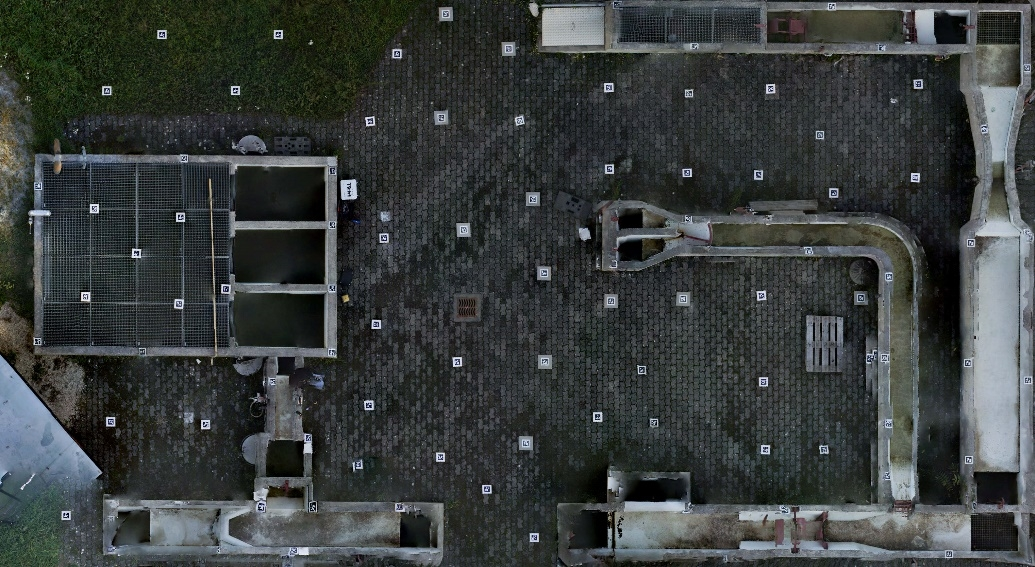
\includegraphics[scale=0.4]{figures/calib_field.png}
    \caption{Scene of the test case.}
    \label{fig:test_case}
\end{figure}
\end{center}


The available information about scene includes:

\begin{itemize}
\item points identified on the photos (approx. 1000 representing 64 object points),
\item position of photos (45) (lever arm offset + object coordinates from GPS unit) 
\item GCPs (7),
\item interior orientation of a camera capturing all photos of the scene.
The camera is first generation of Sony NEX-5 with ultra wide pancake 16 mm lens.
Width of the captured photos was 4592 and height 3056.
The camera contains image sensor with approximate size 25.1 × 16.7 mm.
\end{itemize}
Every parameter also include its standard deviation. 

%%% ML: prvni veta - 2x which
%%% ST: prepsano 

The data contain also protocol of processing done by Bingo-F software \cite{bingo2013gip} revealing 
information about steps performed by the software to retrieve structure of the scene.
Information from the protocol was very helpful for me because 
it gave me first hint about the steps of the processing chain.

Bingo-F is widely used by photogrammetric experts. During its existence, it has proved its qualities on various scenes configurations.  
It is miles ahead compared to the developed processing chain in the thesis therefore the results of the Bingo-F adjustment were 
regarded as reference for obtained data.

Generally, Bingo-F processing chain is very similar to the developed  one  
described in-depth in the previous chapters. First step is the relative orientation of pairs then the pairs are transformed into common relative 
coordinates system. After that, Helmert transformation is performed into world coordinate system. BBA is performed as the last step.

Unlike the developed processing chain, the Bingo-F software takes into account information about position of cameras included in the data. 
Because the developed processing chain should be general as much as possible it was decided that first version of the processing chain would ignore this 
information. According to the set up goals the final solution should require only photo coordinates of tie points and interior 
orientation of cameras. In the future it is possible to extend the processing chain to work with additional information to improve accuracy 
of the results. 

The Bingo-F processing chain is very robust,
capable of identification and ruling out of blunders in individual steps of its processing chain.

Bingo-f protocols reveals following information about performed steps: 
\begin{itemize}
\item Relative orientation -- Algorithm used for calculation of relative orientation is not possible to find out from the protocol.  
\item Transformation to common relative system -- Bingo-F performs so called "Pre-adjustment" of some points. It is probably some type of free network 
BBA. Also during computation of scale, blunder check is preformed inspecting a difference of the object coordinates of points 
used for computation of scale. The difference is calculated between point in common relative system 
and correspondent point determined from relative orientation pair after being transformed into the common relative system.
If standard deviation of the difference is higher than certain threshold, then 
scale is computed again skipping the point with the highest difference and 
transformation into a common system is performed again.
The process is repeated  until  the threshold is satisfied.
\item During BBA iteration it probably sets weights according to information about standard deviation of measured photo points 
and standard deviations of parameters. 
Blunder detection mechanism rules out points with
standard deviation higher than certain threshold. Setting of standard deviation threshold  is common way how to identify 
blunders. It arises from characteristics of normal distribution because probability that measurement occurs with value 
 higher than e.g. 3 standard deviations is extremely small therefore this measurements are considered as blunders in practice.
 
 Another interesting step during Bingo-F BBA is check whether additional parameters improve accuracy. 
 In the first iteration, there are included two additional parameters. After 
 the iteration is performed, it is concluded that the additional parameters have no significance thus 
 they are excluded from further iterations. It is probably related to self-calibration 
 method. Self-calibration can improve accuracy dealing with systematic error mostly caused by 
 distortion. However the presence of the additional parameters may worse overall accuracy in some cases thus 
  the check is performed (more info e.g. in \cite{precision1980grunn}).
\end{itemize}

Bingo-F is highly optimized therefore it allows to solve scenes with thousands of tie points.
The scene was adjusted as a free network refining interior orientation parameters (focal length, principal point coordinates),
exterior orientations of photos and object coordinates of all points (including GCPs). Lever-arm offset is adjusted likewise.
The offset describes 
shift of GPS unit from projective center.  
It allows Bingo-F to use information of photo positions from GPS unit shifted by the offset.  

Reconstructed  scene from Bingo-F results is shown in this plot:

%%% ML: pridal bych popisek

\begin{center}
 \begin{figure}[!h]
    %\centering
    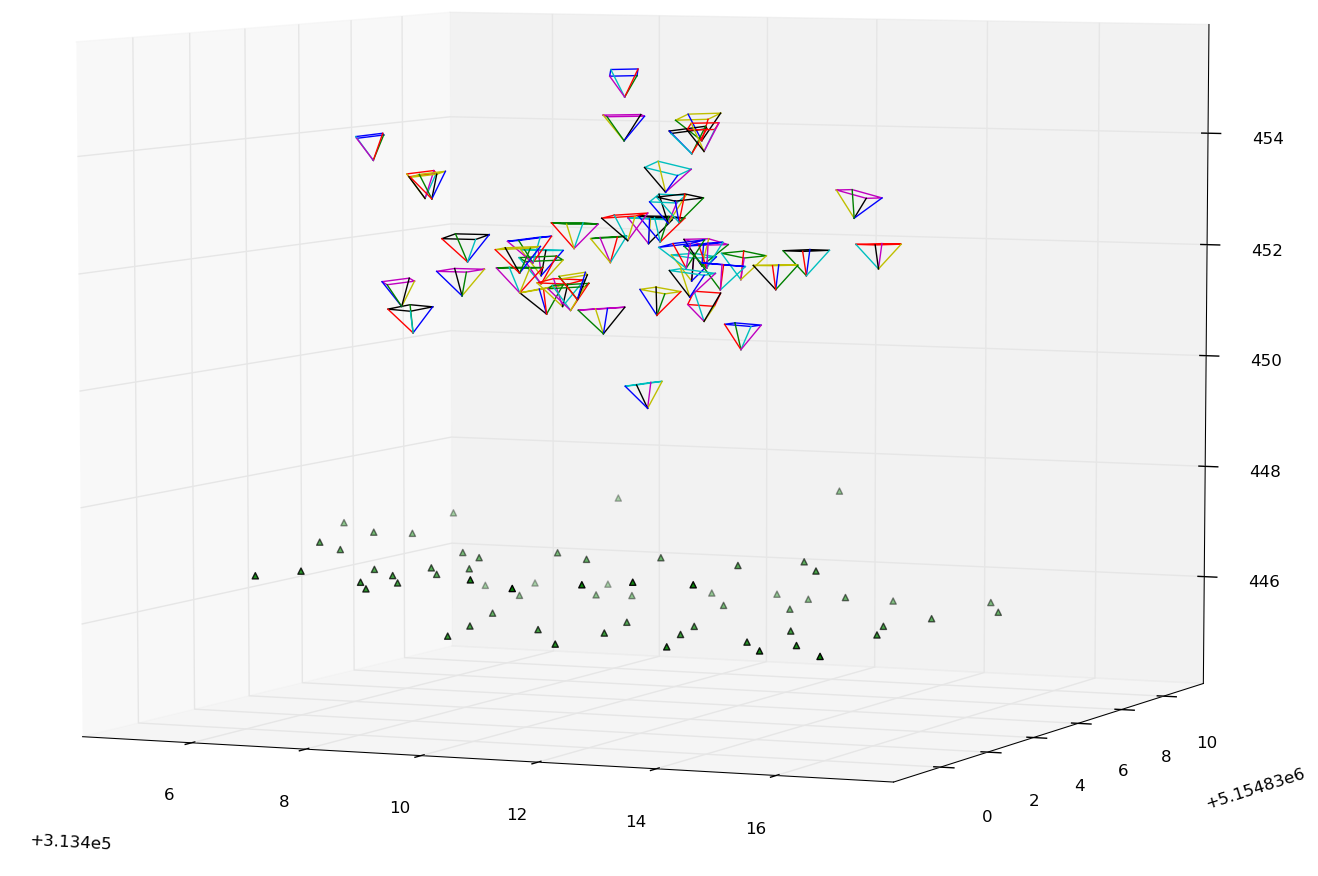
\includegraphics[scale=0.4]{figures/bingo_result.png}
    \caption{Final positions of photos and object points from Bingo-F results.}
    \label{fig:bingo_result}
\end{figure}
\end{center}

Unlike many other scenes, comprised of hundreds of photos and thousands of points,   
there are just a few points (64) and photos (45) taken by same camera. 
The photos capture same points thus there 
is lot of redundancy. Solving such a redundant scene should improve robustness of the BBA. 

In the rest of the chapter, there are presented results of subsequent steps being performed in processing chain and compared 
to the Bingo-F results.

The first step is relative orientation of pairs. The relative orientation of pairs were performed by OpenCV five point algorithm.
The algorithm was successful on most of the pairs, however, there are some cases when the algorithm does not work well.

Example of the algorithm success is showed in this plot:

%%% ML: opet chybi popisek

\begin{center}
 \begin{figure}[!h]
    %\centering
    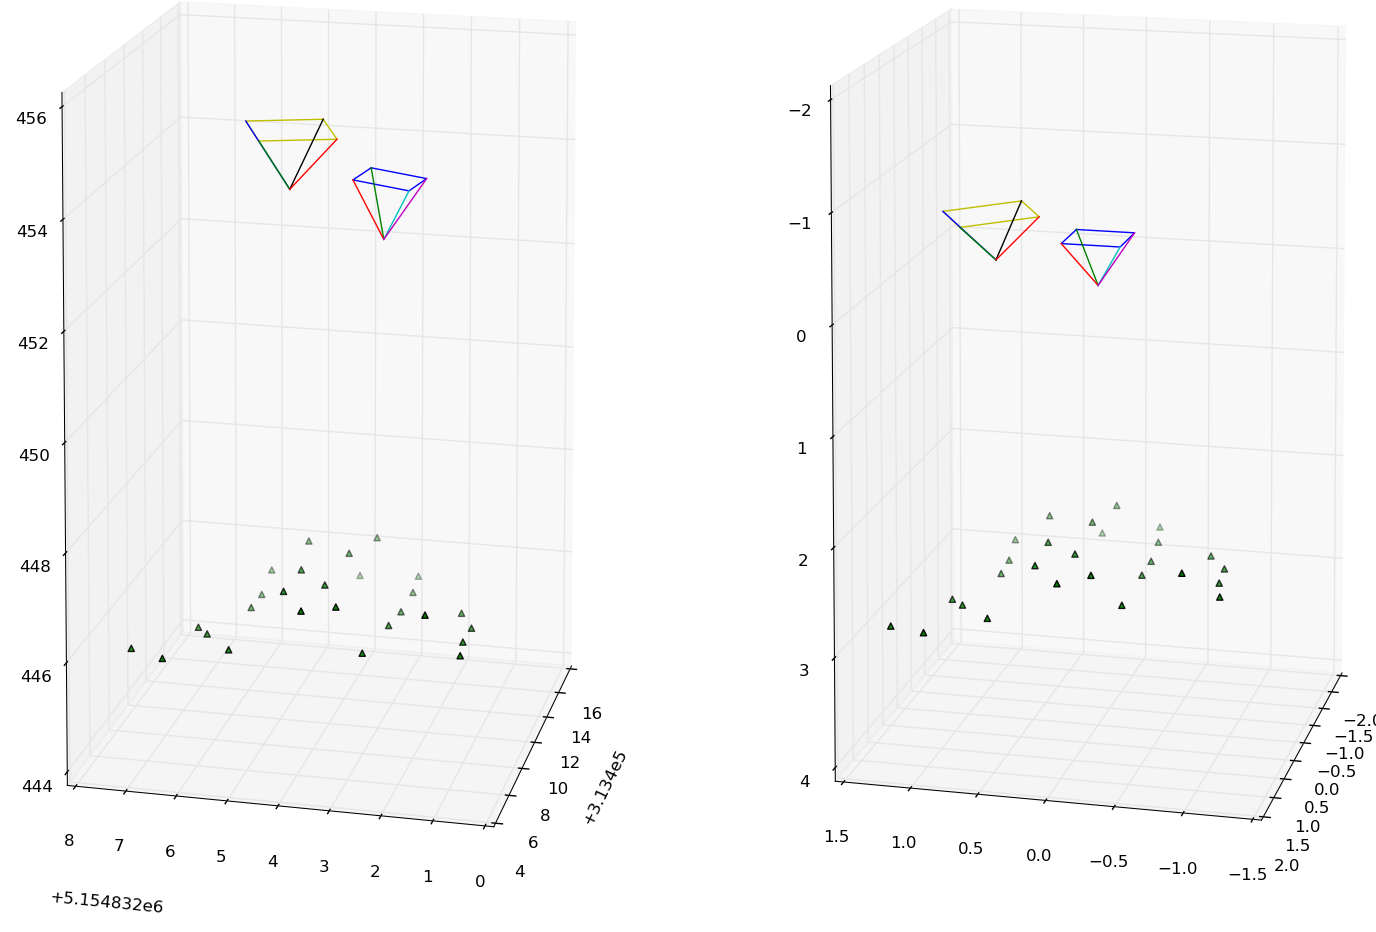
\includegraphics[scale=0.4]{figures/rel_or_576_598.png}
    \caption{Successful relative orientation of photos 576 and 598. In the left picture there 
    is Bingo-F result. The right picture represents the processing chain result.}
    \label{fig:rel_or_ok}
\end{figure}
\end{center}

The right plot shows the result of five point algorithm and the left plot depicts result of Bingo-F. Note that both 
plots are expressed in different coordinate system, however, it is possible to assess them visually. It is clearly visible
that both scenes are very similar.

On the other hand, few relative orientations were unsuccessfully calculated.  
One of such cases is relative orientation of photos pair 553 and 591:  

%%% ML: popisek, viz veta vyse

\begin{center}
 \begin{figure}[!h]
    %\centering
    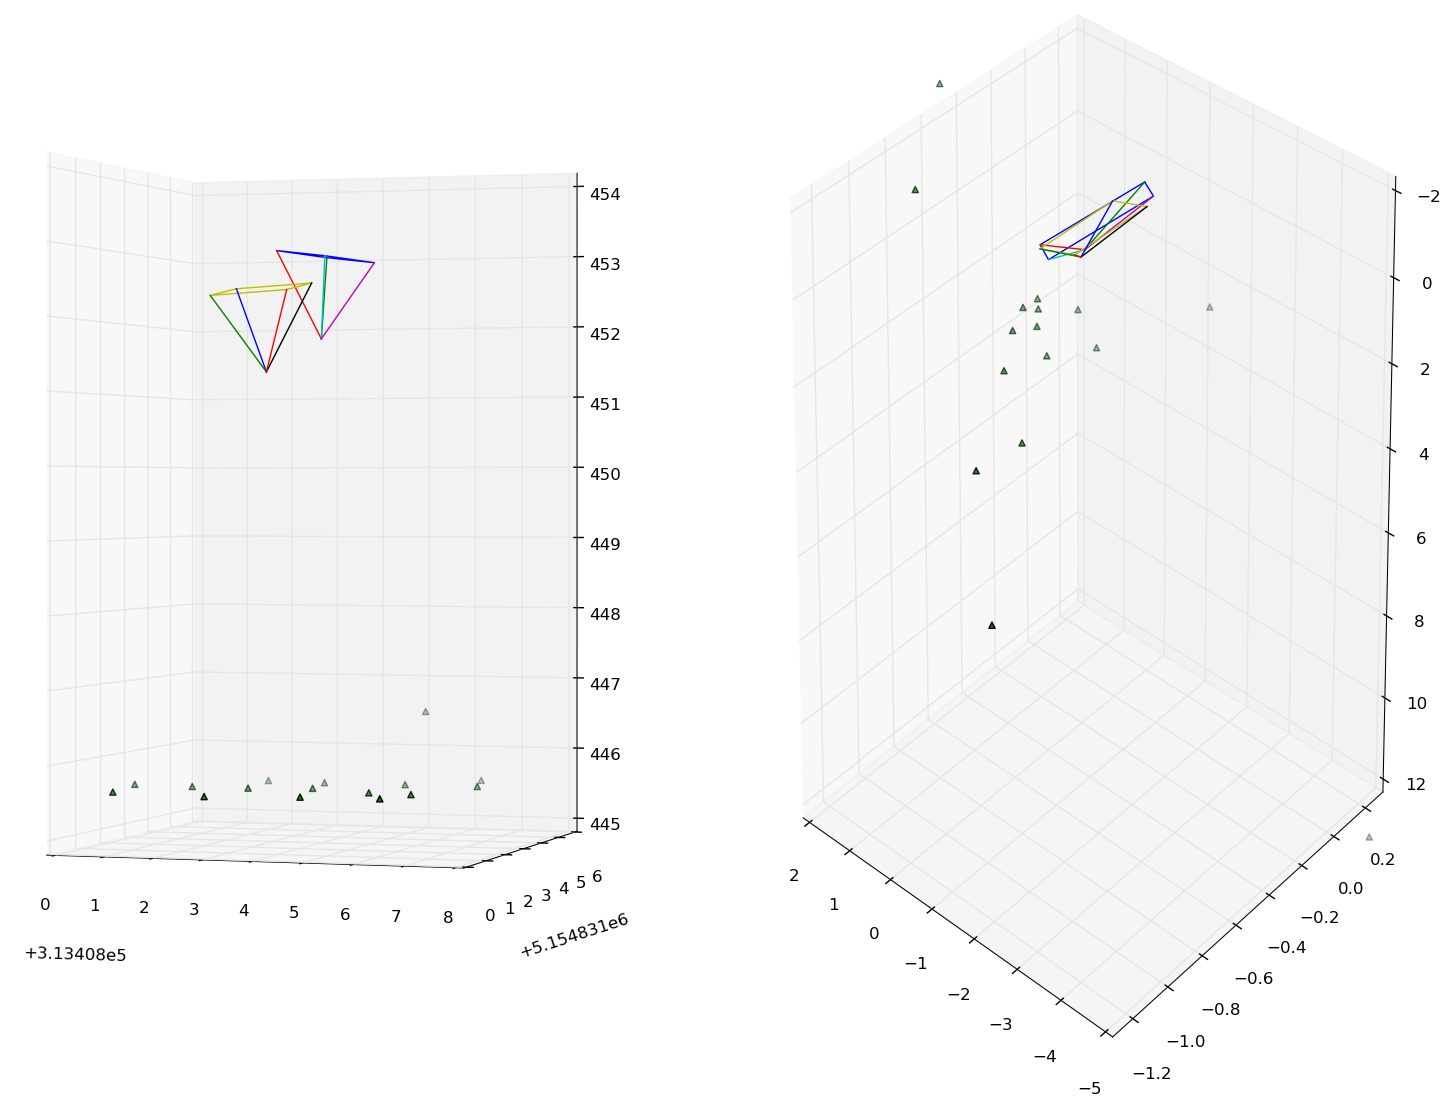
\includegraphics[scale=0.4]{figures/rel_or_553_591.png}
    \caption{Unsuccessful relative orientation of photos 553 and 591. 
    In the left picture there 
    is Bingo-F result. The right picture represents the processing chain result.}
    \label{fig:rel_or_ok}
\end{figure}
\end{center}

It is clearly visible that result of relative orientation is completely different from the Bingo-F final result.
Most important factor, which affects success of the five point algorithm is threshold parameter of RANSAC defining 
whether a point is considered as inlier or outlier.
The above mentioned relative orientations were computed with RANSAC threshold parameters set to 0.001 mm.
If the threshold parameter is changed into 0.1 mm, the result of relative orientation of pair 553 and 591 improves significantly,
but another relative orientations go wrong. Therefore with statically set threshold parameter, there are always 
few evidently wrong relative orientations in the scene. Thanks to the configuration of the photos, where a lot of photos are 
capturing same points, it is  not serious problem because the points are determined in most relative orientations  with 
sufficient accuracy thus it is possible to exclude this outliers. It could be serious problem e.g. if a photos 
of a scene would comprise long chain where redundancy is much more lower thus   
 one wrong relative orientation could thread final result. If error appeared in the middle 
of the chain, it would  be propagated up in one half of the chain  depending on the wrongly
determined pair. It is apparent from equations in \eqref{eq:comm_rel}. 
In the test case, there are not so many critical pairs which has to be determined correctly to avoid spoiling the transformation 
of lot of others dependent pairs. Fortunately the reference pair defining common relative system is very stable and also 
the other core pairs with a lot of depending pairs are stable. 
Probably, there is some correlation between tie point number 
and success rate of RANSAC loop in selection of correct solution. 
Therefore another way how to improve stability of the solution 
could be identification of more tie points. It could be done automatically by pattern matching algorithms. 
In the test case there 
are 27 tie points in the reference pair gradually decreasing 6 points in the pair merged as last.

During the transformation process, all object coordinates representing same point computed from different relative orientations are 
transformed into  the common relative system individually. Then the final coordinates of object points are determined as median
of the corresponding transformed object coordinates. Median was chosen because it is more robust to the effect of 
big outliers caused by few wrong relative orientations in the set. If there are more than 50 percent of coordinates 
close to the correct value and the rest are big outliers (luckily the test data is the case), median gives reasonable results over average
which is much more sensitive to the effect of big outliers. 

%%% ML: veta nize + obrazek - pridal titulek

This plot shows situation before computing median of all corresponding object coordinates:

\begin{center}
 \begin{figure}[!h]
    %\centering
    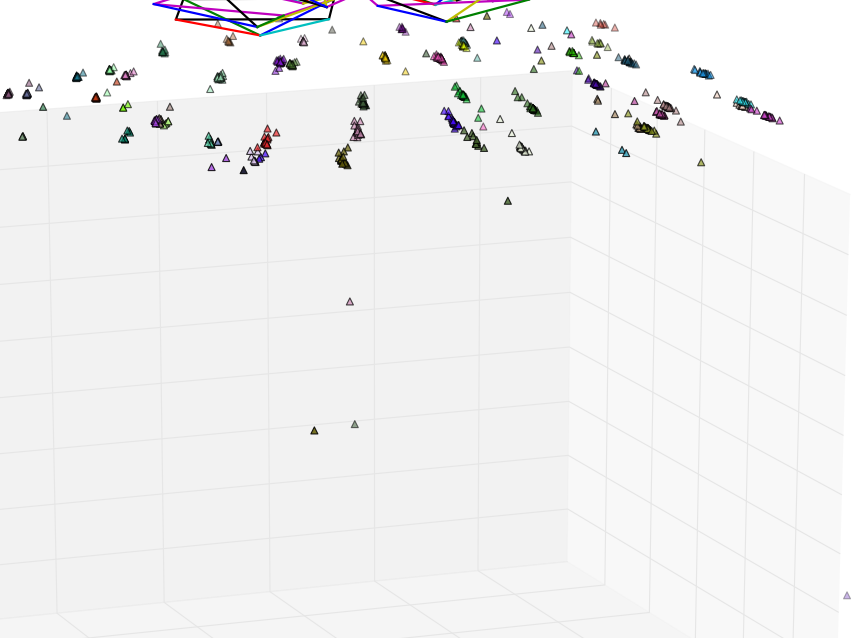
\includegraphics[scale=0.5]{figures/before_median.png}
    \caption{Corresponding object points determined from different relative orientations are represented by same color.}
    \label{fig:rel_or_points}
\end{figure}
\end{center}

Plotted points with same color represent corresponding coordinates computed by different relative orientation. It can be noticed that 
the points of the same color tend to make clusters. However, there are few big outliers whose effect is eliminated by applying
median on the points.

The next step is Helmert transformation of the common relative system into the world coordinate system using available GCPs.
The transformed scene can be finally compared to the results of Bingo-F adjustment.
Average distance of projective center (photos) positions is approx. twenty centimeters. 
The  biggest  outliers are approx. one meter away  
(see table \ref{table:ph_coords_conv}). Angles of exterior orientation differs  generally in average approx. one degree and 
highest outliers reaches nearly 10 degrees of difference (see table \ref{table:ph_angles_conv}). 
The object points coordinates 
are bit closer to Bingo-F results with average approximately 0.08 cm and the highest outliers approx. 0.8 m (See table \ref{table:pt_coords_conv}). 
Angles differences are shown in following plot depicting axes of two camera coordinates systems. One of them represents 
Bingo-F result and another represents
 calculated camera systems before BBA was performed. Both camera coordinates systems originates in calculated projective center coordinates
  before refinement by BBA.
    
%%% ML: obrazek - chybi titulek

\begin{center}
 \begin{figure}[!h]
    %\centering
    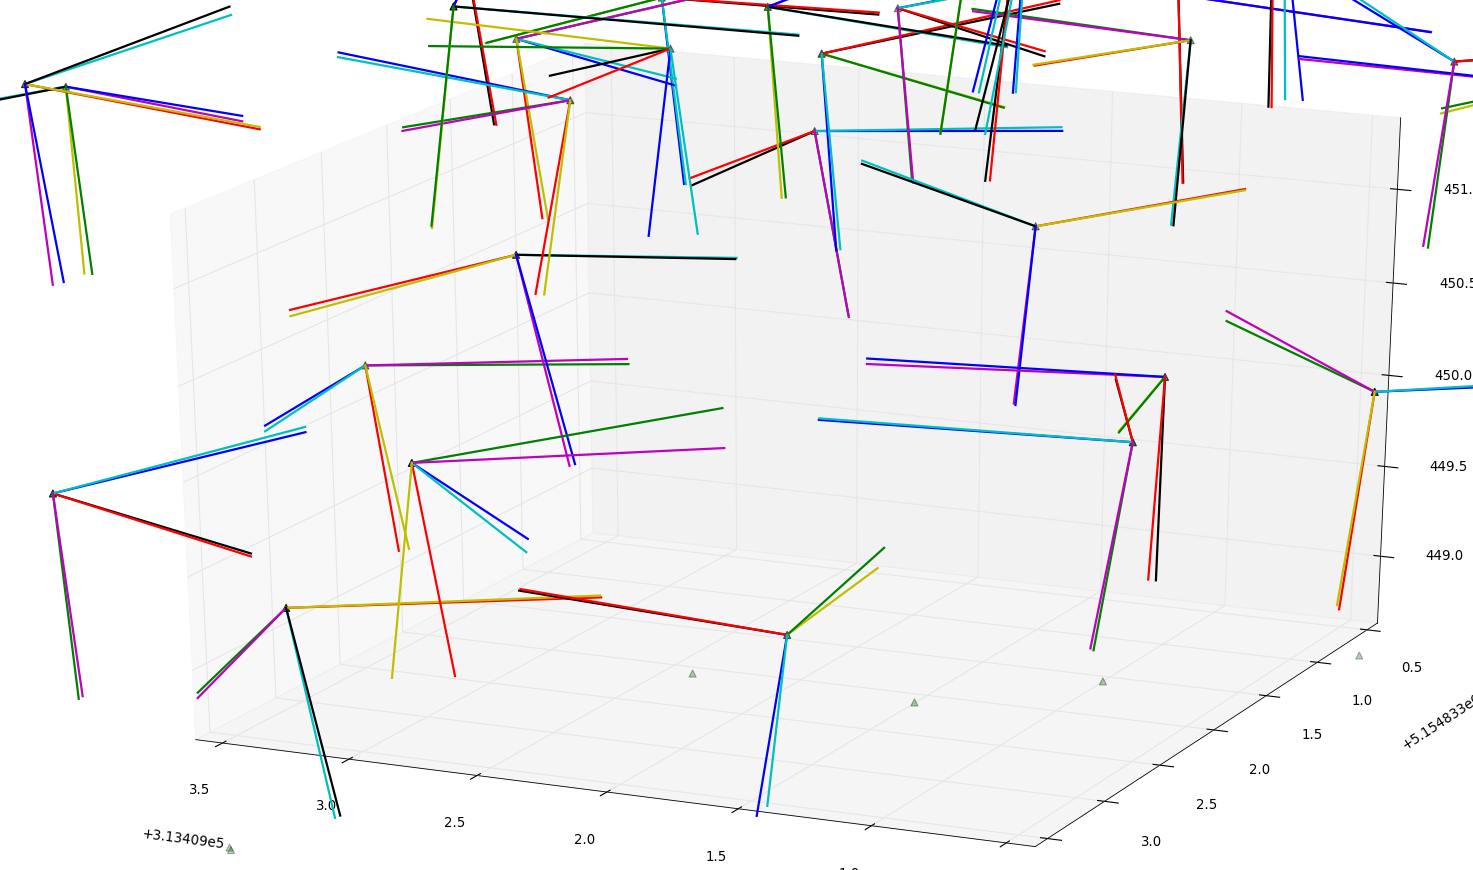
\includegraphics[scale=0.28]{figures/angles_comaprison_relative_orinetaion.png}
     \caption{Camera coordinate systems orientation difference between processing chain result before BBA and Bingo-F final result.}
    \label{fig:cam_diff_bef_bba}
\end{figure}
\end{center}

It is clear that there are few orientations differing in  degrees form the Bingo-F results. 

As the last step BBA was applied beginning with these initial values.
GCPs were taken as knowns.
Despite the fact that there were few huge outliers in both parameters of cameras and points,
BBA subsequently refines all scene parameter and reduces all coordinates 
differences into the centimeters and angles into the tenths of degrees (See tables \ref{table:ph_coords_conv}),
\ref{table:ph_angles_conv}), \ref{table:pt_coords_conv})). 
The BBA iteration is stooped when maximum absolute value in vector of parameters corrections (given in meters and radians) is
smaller than 0.0001.

%%% ML: obrazek - chybi titulek

Following plot shows that differences of cameras coordinates system is no longer being visible from same point of view
unlike to the previous plot:

\begin{center}
 \begin{figure}[!h]
    %\centering
    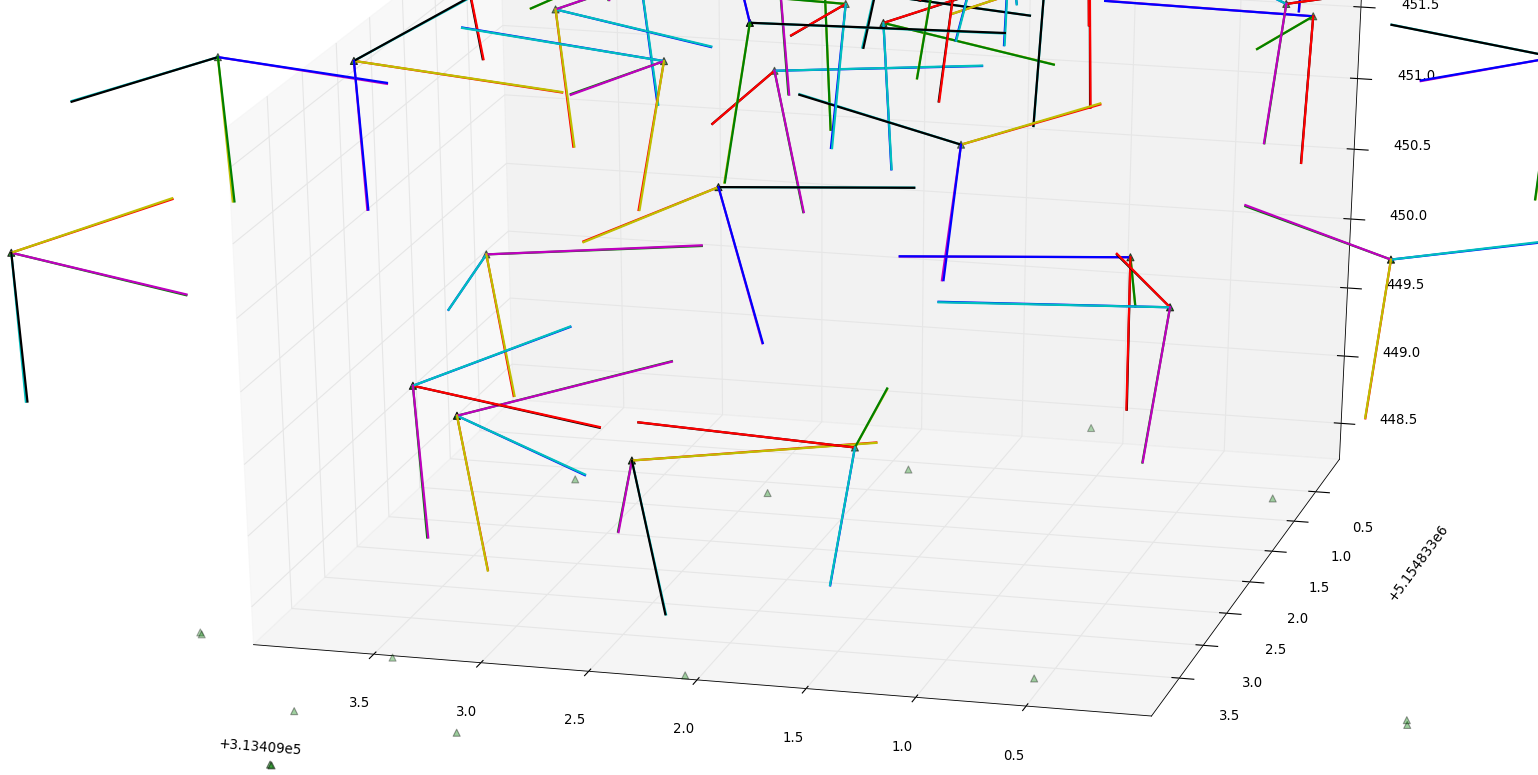
\includegraphics[scale=0.28]{figures/result.png}
     \caption{Camera coordinate systems orientation difference between processing chain final result and Bingo-F final result.}
    \label{fig:cam_diff}
\end{figure}
\end{center}


Whole scene retrieved by processing chain is shown in this plot:

\begin{center}
 \begin{figure}[!h]
    %\centering
      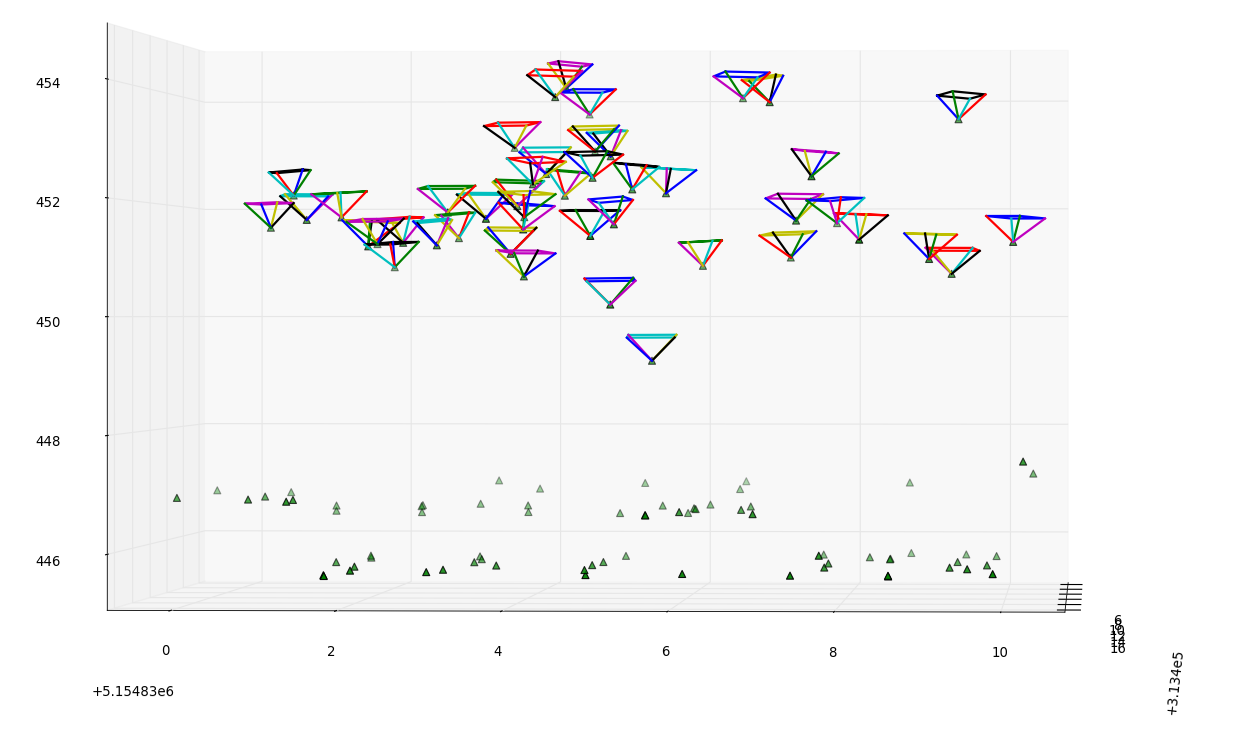
\includegraphics[scale=0.35]{figures/result_all.png}
     \caption{Final scene reconstruction by the developed processing chain.}
    \label{fig:final_result}
\end{figure}
\end{center}

%%% ML: nova kapitola - nova stranka

Median of reprojection error is 1.35 pixel and 90th percentile is 3.34 pixels (see table \ref{table:rep_e_results}).
The reprojection error is computed as difference of measured photo coordinates to 
reprojected object coordinates of points. The statistics are calculated from absolute values of the differences. 

The data contain seven GCPs. Five of them were used for calculation of  Helmert transformation coefficients
likewise they were taken as knowns into the BBA. 
Fixation of GCPs compensate the fact that weight matrix was set to identity. 
Bingo-F uses probably some sophisticated algorithm how to set weights of the measurements because 
clever setting of the weights can significantly improve accuracy obtained from BBA.

Two randomly chosen GCPs were treated as tie points during whole processing. 
Resulting object coordinates were compared to the known coordinates of the two GCPs.
Also same comparison was done with the coordinates from Bingo-F results. 
The coordinates from the processing chain are closer to the known values 
than Bingo-F results (see table \ref{table:comparison}). 
It can not be said that the obtained results 
are more accurate after comparison of just two points. On the other 
hand being closer to real values is  not bad sign at all.
 
If the scene is adjusted as free network without GCPs being fixed and with 
weight matrix given to identity, differences to Bingo-F results increase. 
Mostly it affects exterior orientation.
For instance, average difference in photo position increases from 4.8 cm to 8.4 cm, 


\section{Future development}

The work done in the thesis can be considered as prove of a concept
outlining path of future evolution of current orthorectification workflow in GRASS. 
In the current state the developed 
processing chain can not be considered as generally working solution.

%%% ML: ropbust at all -> robust not enough
%%% ST: opraveno
The processing chain was just tested 
 on one scene where it gives reasonable results. On the other hand 
I am sure that it would not work successfully in other, more complicated scenes because 
it is not robust enough.

In order to improve robustness of the processing chain, following suggestions should be considered:
\begin{itemize}
\item Relative orientations -- there is no check whether relative orientation is successful or not. Some mechanism 
should be implemented assessing quality of relative orientation (probably according to reprojection error of object points or 
epipolar distance).
Also it should be examined work of the five point algorithm with RANSAC loop on scenes with higher number of tie points 
than in the test case where 
the outliers elimination effect of RANSAC loop may be much stronger thanks to bigger sample (points) for testing the
outlier/inlier criterion.
\item  Merging of relative orientations -- if there is one wrong relative orientation with lot of depended relative orientations,
the error gets propagated up during transformation of depended orientations to the common relative coordinate system. 
Effect of such an inaccurate pair could be 
reduced by performing  temporary BBA which can reduce the inaccuracies. Also an order of transformation of relative orientations 
 should not 
be chosen only by number of tie points but also taking into account quality of relative orientation.
Small errors can be serious issue likewise because they can
sum up in long transformation chains. 
\item Calculation of scale -- it is computed as median from individual scales \ref{sec:ess_chain}
without any assessment for outliers. The blunder detection can be implemented in same way 
as in Bingo-F taking into account object coordinates differences of corresponding points used 
for calculation of individual scales.
%%% ML: opet v textu nekolikrat "there exists"
%%% ST: opraveno
\item During final BBA, setting of weights is ignored giving weight matrix equal identity matrix. 
Good choice of weights during every least squares iteration 
could be big leap towards robustness of the BBA and it could also increase accuracy. 
Another way how to improve final accuracy of BBA is skipping photo points with
higher standard deviation than some threshold. The standard deviation criterion can be assessed 
after every iteration.
\end{itemize}


Another big room for improvement is computational speed of the processing chain.
One least squares  iteration of BBA takes approximately 5 seconds in the test case, which can be 
considered as very small scene compared to commonly the solved
scenes with hundreds of photos and thousands of points. Bingo-F manages to go through whole workflow containing 
3 iteration of BBA in just 2 seconds.

The bottleneck of BBA iteration is computation of inverse/pseudo inverse of normal matrix.
The size of the matrix is directly connected to a number of measured photo points.
The inversed matrix of BBA is sparse (most of elements are zeros).
It is possible to use many optimization methods exploiting this property e. g. matrix factorizations. 
Additional speeding up of the code can be achieved by reimplementation of some parts in C programming language 
instead of currently used Python. However, it should be done 
as last step when the part to be reimplemented is tested, optimized and works well. Otherwise, it would be waste of time and energy if the 
code would not be eventually used. 

%%% ML: spa ???, zadny odkaz, stacila by poznamka pod carou...

Another option  for consideration is employing of some free software BBA libraries e.g:
\begin{itemize}
\item sba \footnotetext{http://users.ics.forth.gr/~lourakis/sba/}
\item Simple Sparse Bundle Adjustment \footnotetext{http://www.inf.ethz.ch/personal/chzach/opensource.html}
\end{itemize}

Both libraries are highly optimized, based on Levenberg–Marquardt algorithm.
On the other hand it would require to add new dependency into GRASS. 
Adding new dependencies should be avoided because GRASS already relies on many software libraries
 making its installation difficult because of countless combinations libraries and its versions.
 Moreover it makes fixing of bugs more difficult since some of them
 depend only on certain version of  a library or on a combination of libraries. 
 
The thesis outlines just rough architecture of final solution. At this early stage of development of 
prototype
there is no point in dealing with the interface, which can change lot of time during further development.
It is still needed to define interface of the developed modules to make the modules work not only on the test data. 

Another area for improvement not being covered by the thesis is error analysis of scene parameters and their 
effect on final results. Also it should be studied another non-linear least squares algorithm as e.g. Levenberg–Marquardt or 
Gauss–Newton  algorithms. 

It was set up as one of the main goals that the solution should be general in terms of photos orientation.
The goal was not completely fulfilled because collinearity equations relies on parametrization of camera orientation by Euler angles.
It may cause numerical instabilities in certain direction \ref{sec:eo} thus it must be changed into some other representation.
Unit quaternions seem to be best choice since they do not suffer form gimbal lock problem \cite{schmidt2001using}.

\section{Conclusion}

The path leading into the final solution presented in the thesis has not been straightforward.
In the name of the thesis there is stated that BBA would be 
used only for refining of exterior orientation. When the name had to be chosen in the beginning of this semester, I though that 
it is not big deal. 
I supposed enough GCPs will be 
always available for every photo, interior orientation will be 
known together with initial values of exterior orientation.
This case would require just
performing of BBA.

As I dived more into the topic, it became clear that it would not be so easy 
 if the solution should met up current needs for processing of UAV data.
Thus new goal was set up to come up with a solution as much general 
 as possible allowing to retrieve structure from photos with nearly no other information except interior orientation.
 
The work gave me a chance to get hands on photogrammetry and computer vision. I have become enchanted
by elegance of both fields consisting in a way of building up incredibly powerful methods based on simple principles.  
The simplicity illustrates the fact that the key idea of structure retrieval from photos based on ray intersection
I was able to explain within a five minutes even to my friend with non-technical background of law student who 
  hates mathematics.
Another great thing about the topic is that the results can be assessed
by everybody because it is easy to recognize whether the retrieved structure resembles captured scene or not. 

 The thesis analyzed current state of orthorectification in GRASS and roughly outlined the way of its modification,
 in order to meet up current needs. 
  The developed solution was tested on data comprising of small set of photos capturing a scene.
  The data was also processed in state of the art Bingo-F software whose results were considered as reference.
  After comparison of both results, it can be concluded that the developed processing 
  chain achieved similar accuracy as Bingo-F. However, the solution can be considered just as prove of concept 
  running only on one test case. It is far away from being employed in practice. 


\section{References}

%%% ML: dvakrat se opakuje kapitola "References"

%%% ML: literaturu je dobre rozdelit do dvou sekci - tistena/clanky a
%%% online, ale klidne to nech jak je to ted

\bibliography{DP}
\bibliographystyle{plain}
\bibentry{Hartley2004}

\bibentry{wiki:SIFT}

\bibentry{wiki:SURF}

\bibentry{leutenegger2011brisk}

\bibentry{barazzetti2010extraction}

\bibentry{wiki:Eight-point_algorithm}

\bibentry{stewenius2006recent}

\bibentry{bruckner2008experimental}

\bibentry{nister2004efficient}

\bibentry{pietzsch2001robot}
%TODO
%\bibentry{pietzsch2004application}

\bibentry{rocchini2012robust}

\bibentry{i.ortho.photo}

\bibentry{neteler2008open}

\bibentry{camera_calibration2013opencv}

\bibentry{zhang2000flexible}

\bibentry{calib_manual2013opencv}

\bibentry{v.rectify}

\bibentry{brown1966distortion}

\bibentry{bingo2013gip}

\bibentry{labe2004geometric}

\bibentry{mellish2005pinhole}

\bibentry{boe2013octocopter}

\bibentry{kbosak2010bezmiechowa}

\bibentry{baumker2001new}

\bibentry{sjoberg2013closed}

\bibentry{schmidt2001using}

\bibentry{perry2009synthesized}

\bibentry{pavelka2004foto20}

\bibentry{labe2006automatic}

\bibentry{zhang2004calibration}

\bibentry{strang1997linear}

\bibentry{deakin2006rank}

\bibentry{mikhail1976observations}

\bibentry{mervart2007adjustment}

\bibentry{mathematicalfrederico}

\bibentry{cadaprednaskove}

\bibentry{inductiveload2008selection}

\bibentry{pavelka2004foto10}

\bibentry{neteler2012grass}

\bibentry{rocchini2012let}

\bibentry{heipke1997automation}

\bibentry{precision1980grunn}

\section{Appendix}
\subsection{Adjustment protocol}
\label{sec:adj_protocol}

Following protocol presents results of the developed processing chain
analyzed in chapter \ref{sec:test_case}.

The results were  obtained from non-linear adjustment taking 5 GCPs as knowns.
Two arbitrary GCPs were treated in same way as another tie points 
in the set. The BBA was performed with identity weight matrix. 

Distance between calculated GCP object coordinates  to
 known object coordinates versus distance between object point calculated by  Bingo-F 
 to known coordinates:
\begin{center}
\footnotesize
\rowcolors{1}{}{Gray}
\begin{longtable}{| c || c | c |}
\caption{GCPs coordinate difference (in meters):}
\\ \hline
\label{table:comparison}
GCP. no. & Dev. proc. chain &  Bingo-F \\ \hline 
  2016  &    0.0093  &  0.0296 \\ \hline 
  2023 &     0.0127  &   0.0407 \\ \hline 
  \hline 
\end{longtable}
\end{center}


\begin{center}
\footnotesize
\rowcolors{1}{}{Gray}
\begin{longtable}{| c | c |}
\caption{Reprojection errors statistics calculated 
as absolute values of difference between 
measured photo points and  corresponding photo points 
obtained form adjusted parameters by collinearity equations.
Values are expressed in pixels.}
\label{table:rep_e_results}
\\ \hline
max. & 12.84 \\ \hline 
min. & 0.00 \\ \hline 
avg.  & 1.65 \\ \hline 
perc. 90  & 3.34 \\ \hline 
perc. 75  & 2.36 \\ \hline 
perc. 50  & 1.35 \\ \hline 
perc. 25  & 0.61 \\ \hline 
perc. 10  & 0.24 \\ \hline 
\hline 
\end{longtable}
\end{center}

\subsubsection{Convergence of parameters}

\begin{center} 
%\rowcolors{1}{Gray}{white} 
%\resizebox{10}{10}
%\resizebox{3cm}{!}
\rowcolors{1}{}{Gray}
\footnotesize
\begin{longtable}
{| c || 
c | c | c | c | c | } 
\caption{Distances between object photo positions (projective center position) 
and corresponding photo positions from Bingo-F adjustment.
\term{Bef. I.} column represents distances before BBA iteration was begun.
\term{I. n} column represents distances after \term{n}th BBA iteration.
The distances are expressed in meters.}
\label{table:ph_coords_conv}
\\\hline
Ph. no.&Bef. I.&I. 1 &I. 2 &I. 3 &I. 4 \\ \hline 
\endfirsthead
\multicolumn{3}{@{}l}{\ldots continued}\\\hline
Ph. no.&Bef. I.&I. 1 &I. 2 &I. 3 &I. 4 \\ \hline 
\endhead 
\multicolumn{3}{r@{}}{continued \ldots}\\
\endfoot
\endlastfoot
\hline 
551  &  0.173  &  0.022  &  0.022  &  0.022  &  0.022 \\ \hline 
552  &  0.259  &  0.019  &  0.031  &  0.031  &  0.031 \\ \hline 
553  &  0.059  &  0.032  &  0.031  &  0.031  &  0.031 \\ \hline 
554  &  0.107  &  0.049  &  0.047  &  0.047  &  0.047 \\ \hline 
556  &  0.139  &  0.040  &  0.041  &  0.041  &  0.041 \\ \hline 
557  &  0.191  &  0.044  &  0.049  &  0.049  &  0.049 \\ \hline 
558  &  0.170  &  0.056  &  0.055  &  0.055  &  0.055 \\ \hline 
559  &  1.133  &  0.157  &  0.069  &  0.066  &  0.066 \\ \hline 
560  &  0.172  &  0.064  &  0.036  &  0.037  &  0.037 \\ \hline 
561  &  0.137  &  0.055  &  0.057  &  0.057  &  0.057 \\ \hline 
562  &  0.021  &  0.044  &  0.045  &  0.045  &  0.045 \\ \hline 
563  &  0.100  &  0.044  &  0.048  &  0.048  &  0.048 \\ \hline 
564  &  0.303  &  0.046  &  0.050  &  0.050  &  0.050 \\ \hline 
566  &  0.254  &  0.052  &  0.047  &  0.046  &  0.046 \\ \hline 
567  &  0.190  &  0.043  &  0.046  &  0.046  &  0.046 \\ \hline 
568  &  0.093  &  0.034  &  0.033  &  0.033  &  0.033 \\ \hline 
569  &  0.508  &  0.027  &  0.047  &  0.047  &  0.047 \\ \hline 
570  &  0.084  &  0.047  &  0.049  &  0.049  &  0.049 \\ \hline 
571  &  0.048  &  0.045  &  0.048  &  0.048  &  0.048 \\ \hline 
572  &  0.034  &  0.049  &  0.048  &  0.048  &  0.048 \\ \hline 
573  &  0.057  &  0.040  &  0.043  &  0.043  &  0.043 \\ \hline 
574  &  0.161  &  0.050  &  0.049  &  0.049  &  0.049 \\ \hline 
575  &  0.197  &  0.070  &  0.068  &  0.068  &  0.068 \\ \hline 
576  &  0.110  &  0.052  &  0.055  &  0.055  &  0.055 \\ \hline 
577  &  0.175  &  0.023  &  0.033  &  0.033  &  0.033 \\ \hline 
578  &  0.143  &  0.033  &  0.034  &  0.034  &  0.034 \\ \hline 
579  &  0.109  &  0.046  &  0.045  &  0.045  &  0.045 \\ \hline 
580  &  0.078  &  0.063  &  0.066  &  0.066  &  0.066 \\ \hline 
581  &  0.197  &  0.070  &  0.076  &  0.076  &  0.076 \\ \hline 
582  &  0.114  &  0.061  &  0.065  &  0.065  &  0.065 \\ \hline 
583  &  0.144  &  0.040  &  0.041  &  0.041  &  0.041 \\ \hline 
584  &  0.123  &  0.047  &  0.048  &  0.048  &  0.048 \\ \hline 
585  &  0.046  &  0.051  &  0.053  &  0.053  &  0.053 \\ \hline 
586  &  0.080  &  0.050  &  0.052  &  0.052  &  0.052 \\ \hline 
588  &  0.388  &  0.035  &  0.042  &  0.042  &  0.042 \\ \hline 
589  &  0.334  &  0.067  &  0.061  &  0.061  &  0.061 \\ \hline 
590  &  0.172  &  0.042  &  0.049  &  0.048  &  0.048 \\ \hline 
591  &  1.058  &  0.110  &  0.028  &  0.026  &  0.026 \\ \hline 
592  &  0.165  &  0.035  &  0.037  &  0.037  &  0.037 \\ \hline 
595  &  0.209  &  0.072  &  0.064  &  0.064  &  0.064 \\ \hline 
596  &  0.138  &  0.063  &  0.062  &  0.062  &  0.062 \\ \hline 
597  &  0.196  &  0.058  &  0.060  &  0.060  &  0.060 \\ \hline 
598  &  0.239  &  0.058  &  0.065  &  0.065  &  0.065 \\ \hline 
599  &  0.169  &  0.037  &  0.039  &  0.039  &  0.039 \\ \hline 
600  &  0.351  &  0.041  &  0.041  &  0.041  &  0.041 \\ \hhline{|=|=|=|=|=|=|}
avg. & 0.207 & 0.051 & 0.048 & 0.048 & 0.048 \\ \hline 
max. & 1.133 & 0.157 & 0.076 & 0.076 & 0.076 \\ \hline 
\hline 
\end{longtable}
\end{center}


%%% ML: TODO
\begin{landscape}


\begin{center} 
%\rowcolors{1}{Gray}{white} 
%\resizebox{10}{10}
%\resizebox{3cm}{!}
\footnotesize
\rowcolors{1}{}{Gray}
\begin{longtable}
{|c || c | c | c | c | c || c | c | c | c | c || c | c | c | c | c |} 
\caption{Difference of individual Euler angles ($\varphi$, $\omega$, $\kappa$) between 
calculated angle and corresponding  angle from Bingo-F adjustment.
\label{table:ph_angles_conv}
\term{Bef. I.} column represents differences before BBA iteration was begun.
\term{I. n} column represents differences after \term{n}th BBA iteration.
The differences are expressed in degrees. Last two rows representing average and maximum 
are computed from absolute values of the differences.}
\\\hline
 & \multicolumn{5}{|c||}{$\varphi$}  & \multicolumn{5}{c||}{$\omega$} & \multicolumn{5}{c|}{$\kappa$} \\ \hline 
Ph. no. & Bef. I. & I. 1  & I. 2  & I. 3  & I. 4  & Bef. I. & I. 1  & I. 2  & I. 3  & I. 4  & Bef. I. & I. 1  & I. 2  & I. 3  & I. 4  \\ \hline 
\endfirsthead
\multicolumn{3}{@{}l}{\ldots continued}\\\hline
 & \multicolumn{5}{|c||}{$\varphi$}  & \multicolumn{5}{c||}{$\omega$} & \multicolumn{5}{c|}{$\kappa$} \\ \hline 
Ph. no. & Bef. I. & I. 1  & I. 2  & I. 3  & I. 4  & Bef. I. & I. 1  & I. 2  & I. 3  & I. 4  & Bef. I. & I. 1  & I. 2  & I. 3  & I. 4  \\ \hline 
\endhead 
\multicolumn{3}{r@{}}{continued \ldots}\\
\endfoot
\endlastfoot
551 &  1.441  &  0.263  &  0.256  &  0.256  &  0.256  & -1.862  &  0.010  &  0.013  &  0.013  &  0.013  & -0.266  &  0.065  &  0.034  &  0.033  &  0.033 \\ \hline 
552 &  1.076  &  0.134  &  0.137  &  0.138  &  0.138  &  2.197  &  0.062  &  0.004  &  0.003  &  0.003  & -0.061  &  0.052  &  0.054  &  0.053  &  0.053 \\ \hline 
553 &  0.507  &  0.268  &  0.239  &  0.241  &  0.241  &  0.225  &  0.160  &  0.132  &  0.131  &  0.131  &  0.250  &  0.073  &  0.061  &  0.061  &  0.061 \\ \hline 
554 &  0.907  &  0.296  &  0.285  &  0.286  &  0.286  &  0.686  &  0.235  &  0.189  &  0.189  &  0.189  &  0.291  &  0.071  &  0.054  &  0.054  &  0.054 \\ \hline 
556 &  1.788  &  0.422  &  0.445  &  0.443  &  0.443  & -0.181  & -0.084  & -0.086  & -0.087  & -0.087  &  0.141  &  0.043  &  0.020  &  0.020  &  0.020 \\ \hline 
557 &  0.332  &  0.100  &  0.032  &  0.035  &  0.035  & -1.632  & -0.262  & -0.273  & -0.272  & -0.272  & -0.363  &  0.000  & -0.008  & -0.008  & -0.008 \\ \hline 
558 &  0.286  & -0.220  & -0.220  & -0.215  & -0.215  & -1.492  & -0.321  & -0.175  & -0.172  & -0.171  & -0.267  &  0.082  &  0.091  &  0.090  &  0.090 \\ \hline 
559 & -9.639  &  0.338  &  0.013  &  0.055  &  0.055  &  5.244  &  0.696  &  0.278  &  0.297  &  0.297  & -0.067  &  0.542  &  0.021  &  0.035  &  0.035 \\ \hline 
560 & -0.102  &  0.033  &  0.258  &  0.251  &  0.251  & -1.663  &  0.330  & -0.029  & -0.010  & -0.011  & -0.066  &  0.093  &  0.065  &  0.067  &  0.067 \\ \hline 
561 &  0.426  &  0.060  &  0.010  &  0.012  &  0.012  & -1.003  & -0.250  & -0.258  & -0.258  & -0.258  & -0.179  &  0.066  &  0.053  &  0.053  &  0.053 \\ \hline 
562 & -0.036  &  0.163  &  0.115  &  0.117  &  0.117  &  0.243  & -0.025  & -0.046  & -0.046  & -0.046  & -0.184  &  0.046  &  0.042  &  0.042  &  0.042 \\ \hline 
563 &  0.650  &  0.009  & -0.043  & -0.041  & -0.041  & -0.533  & -0.038  & -0.043  & -0.043  & -0.043  & -0.240  &  0.055  &  0.039  &  0.039  &  0.039 \\ \hline 
564 &  1.162  &  0.216  &  0.189  &  0.191  &  0.191  & -2.160  & -0.193  & -0.203  & -0.203  & -0.203  & -0.047  &  0.079  &  0.060  &  0.060  &  0.060 \\ \hline 
566 &  1.222  &  0.231  &  0.362  &  0.347  &  0.347  & -2.109  &  0.144  & -0.202  & -0.180  & -0.180  &  0.107  &  0.111  &  0.087  &  0.088  &  0.088 \\ \hline 
567 &  1.855  &  0.307  &  0.270  &  0.271  &  0.271  &  1.012  & -0.067  & -0.078  & -0.080  & -0.080  &  0.039  &  0.055  &  0.062  &  0.062  &  0.062 \\ \hline 
568 &  0.921  &  0.355  &  0.305  &  0.307  &  0.307  &  1.475  &  0.326  &  0.289  &  0.291  &  0.291  &  0.116  &  0.039  &  0.045  &  0.045  &  0.045 \\ \hline 
569 & -4.150  &  0.279  &  0.083  &  0.086  &  0.086  &  0.007  &  0.162  &  0.330  &  0.331  &  0.331  &  0.339  &  0.002  &  0.072  &  0.072  &  0.072 \\ \hline 
570 &  0.906  & -0.012  & -0.036  & -0.034  & -0.034  &  0.407  & -0.027  & -0.026  & -0.025  & -0.025  & -0.166  &  0.043  &  0.049  &  0.049  &  0.049 \\ \hline 
571 &  0.385  &  0.007  & -0.059  & -0.059  & -0.059  &  0.579  &  0.210  &  0.198  &  0.199  &  0.199  & -0.235  &  0.030  &  0.045  &  0.045  &  0.045 \\ \hline 
572 &  0.272  & -0.069  & -0.058  & -0.057  & -0.057  & -0.047  &  0.235  &  0.244  &  0.244  &  0.244  & -0.338  &  0.034  &  0.039  &  0.039  &  0.039 \\ \hline 
573 &  0.703  & -0.000  & -0.036  & -0.034  & -0.034  &  0.369  &  0.065  &  0.043  &  0.044  &  0.044  & -0.214  &  0.057  &  0.053  &  0.053  &  0.053 \\ \hline 
574 &  1.554  &  0.211  &  0.200  &  0.201  &  0.201  & -0.827  & -0.257  & -0.256  & -0.256  & -0.256  &  0.106  &  0.081  &  0.060  &  0.060  &  0.060 \\ \hline 
575 & -0.662  &  0.151  &  0.108  &  0.110  &  0.110  & -1.039  & -0.332  & -0.308  & -0.308  & -0.308  & -0.198  &  0.045  &  0.062  &  0.062  &  0.062 \\ \hline 
576 &  0.274  &  0.144  &  0.112  &  0.114  &  0.114  & -0.809  & -0.159  & -0.211  & -0.209  & -0.209  & -0.078  &  0.048  &  0.041  &  0.041  &  0.041 \\ \hline 
577 & -0.937  &  0.081  &  0.062  &  0.067  &  0.067  &  1.447  &  0.271  & -0.039  & -0.040  & -0.040  & -0.031  &  0.080  &  0.055  &  0.054  &  0.054 \\ \hline 
578 & -0.759  & -0.048  & -0.072  & -0.071  & -0.071  &  0.915  &  0.309  &  0.259  &  0.261  &  0.261  &  0.141  &  0.005  &  0.018  &  0.018  &  0.018 \\ \hline 
579 & -0.693  & -0.014  & -0.034  & -0.033  & -0.033  &  0.562  &  0.491  &  0.452  &  0.453  &  0.453  &  0.076  &  0.016  &  0.012  &  0.012  &  0.012 \\ \hline 
580 & -0.513  & -0.203  & -0.228  & -0.226  & -0.226  & -0.014  &  0.140  &  0.109  &  0.110  &  0.110  &  0.084  &  0.044  &  0.033  &  0.033  &  0.033 \\ \hline 
581 & -1.166  & -0.268  & -0.305  & -0.304  & -0.304  & -0.176  &  0.124  &  0.111  &  0.112  &  0.112  &  0.023  &  0.031  &  0.025  &  0.025  &  0.025 \\ \hline 
582 & -0.692  & -0.208  & -0.246  & -0.245  & -0.245  & -0.213  &  0.116  &  0.094  &  0.095  &  0.095  &  0.024  &  0.039  &  0.030  &  0.030  &  0.030 \\ \hline 
583 &  1.233  &  0.174  &  0.154  &  0.156  &  0.156  & -0.250  &  0.030  &  0.015  &  0.015  &  0.015  &  0.060  &  0.060  &  0.046  &  0.046  &  0.046 \\ \hline 
584 &  0.700  &  0.138  &  0.123  &  0.125  &  0.125  & -0.842  & -0.112  & -0.130  & -0.130  & -0.130  & -0.023  &  0.065  &  0.052  &  0.052  &  0.052 \\ \hline 
585 &  0.169  &  0.084  &  0.051  &  0.053  &  0.053  &  0.287  & -0.063  & -0.083  & -0.083  & -0.083  &  0.002  &  0.061  &  0.055  &  0.055  &  0.055 \\ \hline 
586 &  0.745  &  0.412  &  0.382  &  0.383  &  0.383  &  0.808  & -0.255  & -0.285  & -0.286  & -0.286  & -0.015  &  0.058  &  0.048  &  0.049  &  0.049 \\ \hline 
588 & -2.853  &  0.459  &  0.333  &  0.335  &  0.335  & -1.393  &  0.054  &  0.037  &  0.036  &  0.036  &  0.548  & -0.048  &  0.020  &  0.020  &  0.020 \\ \hline 
589 & -1.369  & -0.133  & -0.131  & -0.129  & -0.130  & -2.510  & -0.595  & -0.477  & -0.475  & -0.474  &  0.255  &  0.047  &  0.065  &  0.066  &  0.066 \\ \hline 
590 & -1.251  & -0.062  & -0.114  & -0.112  & -0.112  & -0.580  & -0.033  & -0.067  & -0.068  & -0.068  & -0.261  &  0.035  &  0.034  &  0.034  &  0.034 \\ \hline 
591 &  8.499  &  0.600  &  0.347  &  0.359  &  0.359  & -6.446  &  0.552  &  0.109  &  0.127  &  0.127  &  0.130  &  0.727  &  0.032  &  0.047  &  0.047 \\ \hline 
592 & -1.585  & -0.132  & -0.145  & -0.143  & -0.143  &  0.023  & -0.145  & -0.144  & -0.143  & -0.143  & -0.121  &  0.039  &  0.047  &  0.047  &  0.047 \\ \hline 
595 & -0.648  &  0.075  &  0.075  &  0.078  &  0.078  & -1.055  & -0.338  & -0.211  & -0.213  & -0.213  & -0.032  &  0.062  &  0.068  &  0.068  &  0.068 \\ \hline 
596 & -0.157  &  0.272  &  0.253  &  0.254  &  0.254  & -0.568  &  0.055  &  0.072  &  0.073  &  0.073  & -0.459  &  0.021  &  0.022  &  0.022  &  0.022 \\ \hline 
597 &  1.419  &  0.332  &  0.316  &  0.317  &  0.317  &  0.022  &  0.219  &  0.219  &  0.220  &  0.220  &  0.056  &  0.034  &  0.025  &  0.025  &  0.025 \\ \hline 
598 &  0.404  &  0.173  &  0.117  &  0.119  &  0.119  & -1.519  & -0.233  & -0.271  & -0.271  & -0.271  &  0.078  &  0.076  &  0.070  &  0.070  &  0.070 \\ \hline 
599 & -1.027  &  0.057  &  0.004  &  0.007  &  0.007  & -0.986  & -0.383  & -0.378  & -0.378  & -0.378  &  0.211  &  0.041  &  0.052  &  0.052  &  0.052 \\ \hline 
600 & -0.794  & -0.052  & -0.118  & -0.115  & -0.115  & -6.775  & -0.247  & -0.265  & -0.265  & -0.265  & -0.707  &  0.017  &  0.060  &  0.059  &  0.059 \\ \hhline{|=|=|=|=|=|=|=|=|=|=|=|=|=|=|=|=|} 
avg. &  1.308  &  0.184  &  0.166  &  0.167  &  0.167  &  1.226  &  0.209  &  0.172  &  0.172  &  0.172  &  0.171  &  0.076  &  0.046  &  0.047  &  0.047 \\ \hline 
max. &  9.639  &  0.600  &  0.445  &  0.443  &  0.443  &  6.775  &  0.696  &  0.477  &  0.475  &  0.474  &  0.707  &  0.727  &  0.091  &  0.090  &  0.090 \\ \hline 
\hline 
\end{longtable}
\end{center}
\end{landscape}

%%% ML: TODO
\begin{center} 
%\rowcolors{1}{Gray}{white} 
%\resizebox{10}{10}
%\resizebox{3cm}{!}
\footnotesize
\rowcolors{1}{}{Gray}
\begin{longtable}
{| c || 
c | c | c | c | c | } 
\caption{Distance between adjusted points object coordinates and corresponding points
from Bingo-F adjustment.
\term{Bef. I.} column represents differences before BBA iteration was begun.
\term{I. n} column represents differences after \term{n}th BBA iteration.
The distances are expressed in meters.}
\label{table:pt_coords_conv}
\\ \hline 
Ph. no.&Bef. I.&I. 1 &I. 2 &I. 3 &I. 4 \\ \hline 
\endfirsthead
\multicolumn{3}{@{}l}{\ldots continued}\\\hline
Ph. no.&Bef. I.&I. 1 &I. 2 &I. 3 &I. 4 \\ \hline 
\endhead 
\multicolumn{3}{r@{}}{continued \ldots}\\
\endfoot
\endlastfoot
\hline 
2005  &  0.052  &  0.052  &  0.050  &  0.050  &  0.050 \\ \hline 
2007  &  0.094  &  0.021  &  0.029  &  0.029  &  0.029 \\ \hline 
2008  &  0.036  &  0.069  &  0.066  &  0.066  &  0.066 \\ \hline 
2010  &  0.088  &  0.049  &  0.054  &  0.054  &  0.054 \\ \hline 
2014  &  0.155  &  0.057  &  0.036  &  0.037  &  0.037 \\ \hline 
2015  &  0.082  &  0.037  &  0.032  &  0.032  &  0.032 \\ \hline 
2016  &  0.057  &  0.039  &  0.038  &  0.038  &  0.038 \\ \hline 
2018  &  0.050  &  0.025  &  0.027  &  0.027  &  0.027 \\ \hline 
2020  &  0.031  &  0.034  &  0.033  &  0.033  &  0.033 \\ \hline 
2023  &  0.017  &  0.032  &  0.035  &  0.035  &  0.035 \\ \hline 
2024  &  0.037  &  0.044  &  0.043  &  0.043  &  0.043 \\ \hline 
2026  &  0.060  &  0.047  &  0.043  &  0.043  &  0.043 \\ \hline 
2027  &  0.024  &  0.038  &  0.040  &  0.040  &  0.040 \\ \hline 
2029  &  0.093  &  0.052  &  0.050  &  0.050  &  0.050 \\ \hline 
2031  &  0.018  &  0.045  &  0.046  &  0.045  &  0.045 \\ \hline 
2033  &  0.040  &  0.011  &  0.011  &  0.011  &  0.011 \\ \hline 
2036  &  0.141  &  0.029  &  0.030  &  0.030  &  0.030 \\ \hline 
2038  &  0.775  &  0.132  &  0.033  &  0.031  &  0.031 \\ \hline 
2041  &  0.111  &  0.014  &  0.012  &  0.011  &  0.011 \\ \hline 
2050  &  0.024  &  0.017  &  0.018  &  0.018  &  0.018 \\ \hline 
2054  &  0.052  &  0.026  &  0.026  &  0.026  &  0.026 \\ \hline 
2057  &  0.079  &  0.037  &  0.035  &  0.035  &  0.035 \\ \hline 
2059  &  0.021  &  0.019  &  0.020  &  0.020  &  0.020 \\ \hline 
2060  &  0.141  &  0.041  &  0.039  &  0.039  &  0.039 \\ \hline 
2062  &  0.064  &  0.028  &  0.030  &  0.029  &  0.029 \\ \hline 
2064  &  0.079  &  0.052  &  0.051  &  0.051  &  0.051 \\ \hline 
2066  &  0.042  &  0.017  &  0.016  &  0.016  &  0.016 \\ \hline 
2067  &  0.102  &  0.033  &  0.032  &  0.032  &  0.032 \\ \hline 
2074  &  0.067  &  0.048  &  0.047  &  0.047  &  0.047 \\ \hline 
2077  &  0.060  &  0.038  &  0.039  &  0.039  &  0.039 \\ \hline 
2079  &  0.066  &  0.044  &  0.044  &  0.044  &  0.044 \\ \hline 
2082  &  0.087  &  0.052  &  0.053  &  0.053  &  0.053 \\ \hline 
2085  &  0.024  &  0.023  &  0.025  &  0.025  &  0.025 \\ \hline 
2086  &  0.525  &  0.068  &  0.041  &  0.041  &  0.041 \\ \hline 
2087  &  0.087  &  0.057  &  0.058  &  0.058  &  0.058 \\ \hline 
2088  &  0.059  &  0.044  &  0.042  &  0.042  &  0.042 \\ \hline 
2089  &  0.046  &  0.055  &  0.052  &  0.052  &  0.052 \\ \hline 
2090  &  0.024  &  0.045  &  0.044  &  0.044  &  0.044 \\ \hline 
2093  &  0.094  &  0.021  &  0.021  &  0.021  &  0.021 \\ \hline 
2095  &  0.015  &  0.033  &  0.034  &  0.034  &  0.034 \\ \hline 
2099  &  0.171  &  0.019  &  0.021  &  0.021  &  0.021 \\ \hline 
2100  &  0.042  &  0.043  &  0.042  &  0.042  &  0.042 \\ \hline 
2102  &  0.092  &  0.054  &  0.054  &  0.054  &  0.054 \\ \hline 
2103  &  0.048  &  0.044  &  0.044  &  0.044  &  0.044 \\ \hline 
2104  &  0.042  &  0.016  &  0.018  &  0.018  &  0.018 \\ \hline 
2105  &  0.050  &  0.006  &  0.007  &  0.007  &  0.007 \\ \hline 
2107  &  0.081  &  0.067  &  0.065  &  0.064  &  0.064 \\ \hline 
2108  &  0.095  &  0.052  &  0.055  &  0.055  &  0.055 \\ \hline 
2110  &  0.077  &  0.051  &  0.051  &  0.051  &  0.051 \\ \hline 
2112  &  0.056  &  0.056  &  0.053  &  0.053  &  0.053 \\ \hline 
2114  &  0.180  &  0.039  &  0.039  &  0.039  &  0.039 \\ \hline 
2116  &  0.097  &  0.054  &  0.054  &  0.054  &  0.054 \\ \hline 
2117  &  0.024  &  0.029  &  0.032  &  0.032  &  0.032 \\ \hline 
2119  &  0.061  &  0.053  &  0.054  &  0.054  &  0.054 \\ \hline 
2120  &  0.077  &  0.054  &  0.054  &  0.054  &  0.054 \\ \hline 
2122  &  0.060  &  0.037  &  0.037  &  0.037  &  0.037 \\ \hline 
2123  &  0.110  &  0.064  &  0.065  &  0.065  &  0.065 \\ \hline 
2125  &  0.070  &  0.045  &  0.047  &  0.047  &  0.047 \\ \hline 
2127  &  0.092  &  0.018  &  0.023  &  0.023  &  0.023 \\ \hhline{|=|=|=|=|=|=|}
avg. & 0.089 & 0.041 & 0.039 & 0.039 & 0.039 \\ \hline 
max. & 0.775 & 0.132 & 0.066 & 0.066 & 0.066 \\ \hline 
\hline 
\end{longtable}
\end{center}

\begin{landscape}
\subsubsection{Results}
\begin{center} 
%\rowcolors{1}{Gray}{white} 
%\resizebox{10}{10}
%\resizebox{3cm}{!}
\footnotesize
\rowcolors{1}{}{Gray}
\hspace*{-1.5in}
\begin{longtable}
{| c || 
c | c | c | c | c | c | c | c | c | c | c | c |} 
\caption{Final results of exterior orientation (projective center object coordinates $X$, $Y$, $Z$  and Euler angles $\varphi$, $\omega$, $\kappa$)
including standard deviations $\sigma$ calculated from adjustment. 
Angles are expressed in degrees and coordinates in  meters (same applies for corresponding $\sigma$).}
\label{table:eo_results}
\\\hline
$Ph. no.$ & $\varphi$ & $\sigma_{\varphi}$ & $\omega$ & $\sigma_{\omega}$ & $\kappa$ & $\sigma_{\kappa}$  & $X$ & $\sigma_{X}$  & $Y$ & $\sigma_{Y}$ & $Z$ & $\sigma_{Z}$  \\ \hline 
\endfirsthead
\multicolumn{3}{@{}l}{\ldots continued}\\\hline
$Ph. no.$ & $\varphi$ & $\sigma_{\varphi}$ & $\omega$ & $\sigma_{\omega}$ & $\kappa$ & $\sigma_{\kappa}$  & $X$ & $\sigma_{X}$  & $Y$ & $\sigma_{Y}$ & $Z$ & $\sigma_{Z}$  \\ \hline 
\endhead 
\multicolumn{3}{r@{}}{continued \ldots}\\
\endfoot
\endlastfoot
\hline
551 &     6.741 &      0.111  &      0.209 &      0.079  &     96.952 &      0.037  & 313412.527 &      0.009  & 5154835.072 &      0.007  &    450.211 &      0.003  \\ \hline 
552 &     7.860 &      0.093  &     -0.470 &      0.093  &     88.484 &      0.030  & 313411.514 &      0.009  & 5154833.755 &      0.010  &    451.107 &      0.003  \\ \hline 
553 &     5.145 &      0.070  &      0.397 &      0.076  &     76.560 &      0.024  & 313412.235 &      0.008  & 5154833.493 &      0.009  &    451.714 &      0.003  \\ \hline 
554 &     7.432 &      0.085  &      1.643 &      0.080  &     77.773 &      0.028  & 313413.239 &      0.009  & 5154833.088 &      0.009  &    451.808 &      0.004  \\ \hline 
556 &     2.635 &      0.100  &      0.358 &      0.064  &     67.429 &      0.028  & 313413.827 &      0.011  & 5154834.897 &      0.007  &    451.393 &      0.003  \\ \hline 
557 &    11.644 &      0.104  &      2.546 &      0.077  &     71.512 &      0.030  & 313410.808 &      0.011  & 5154837.337 &      0.009  &    451.700 &      0.005  \\ \hline 
558 &     7.100 &      0.182  &     -1.742 &      0.289  &    102.532 &      0.075  & 313410.643 &      0.017  & 5154839.308 &      0.026  &    450.758 &      0.010  \\ \hline 
559 &     4.953 &      0.106  &     -4.124 &      0.105  &    136.262 &      0.046  & 313411.136 &      0.012  & 5154840.093 &      0.010  &    451.317 &      0.007  \\ \hline 
560 &     1.645 &      0.071  &     -2.565 &      0.132  &    155.802 &      0.036  & 313411.647 &      0.008  & 5154839.041 &      0.012  &    451.012 &      0.004  \\ \hline 
561 &     1.198 &      0.071  &     -4.644 &      0.064  &    150.711 &      0.022  & 313410.516 &      0.009  & 5154835.670 &      0.007  &    452.192 &      0.003  \\ \hline 
562 &    -0.427 &      0.067  &     -6.829 &      0.087  &    170.906 &      0.024  & 313409.904 &      0.008  & 5154834.343 &      0.010  &    452.161 &      0.003  \\ \hline 
563 &    -0.088 &      0.070  &     -6.517 &      0.076  &    167.398 &      0.024  & 313410.886 &      0.009  & 5154835.260 &      0.009  &    452.254 &      0.003  \\ \hline 
564 &     0.141 &      0.075  &     -6.256 &      0.076  &    166.403 &      0.026  & 313412.314 &      0.010  & 5154837.583 &      0.009  &    452.452 &      0.004  \\ \hline 
566 &     0.364 &      0.103  &     -2.887 &      0.127  &    155.673 &      0.040  & 313413.658 &      0.011  & 5154838.216 &      0.013  &    451.328 &      0.005  \\ \hline 
567 &     2.697 &      0.076  &     -5.730 &      0.131  &    150.703 &      0.029  & 313412.494 &      0.008  & 5154833.979 &      0.014  &    451.523 &      0.003  \\ \hline 
568 &     1.919 &      0.089  &     -4.601 &      0.119  &    146.954 &      0.036  & 313411.965 &      0.009  & 5154831.987 &      0.012  &    451.235 &      0.005  \\ \hline 
569 &     5.771 &      0.085  &     -0.115 &      0.115  &     87.515 &      0.037  & 313411.086 &      0.009  & 5154831.131 &      0.012  &    451.713 &      0.007  \\ \hline 
570 &     2.072 &      0.077  &      4.277 &      0.091  &     37.892 &      0.028  & 313410.552 &      0.009  & 5154831.528 &      0.010  &    451.766 &      0.004  \\ \hline 
571 &    -0.291 &      0.072  &      6.769 &      0.090  &     -4.402 &      0.030  & 313409.647 &      0.009  & 5154830.832 &      0.010  &    452.173 &      0.004  \\ \hline 
572 &    -1.143 &      0.078  &      2.858 &      0.103  &    -14.821 &      0.035  & 313409.669 &      0.009  & 5154830.540 &      0.010  &    451.595 &      0.004  \\ \hline 
573 &    -1.167 &      0.073  &      5.375 &      0.085  &    -12.498 &      0.026  & 313410.574 &      0.008  & 5154832.318 &      0.008  &    451.313 &      0.003  \\ \hline 
574 &    -5.547 &      0.084  &      5.536 &      0.084  &     -9.076 &      0.031  & 313411.674 &      0.009  & 5154835.070 &      0.009  &    451.624 &      0.003  \\ \hline 
575 &    -0.950 &      0.075  &     11.991 &      0.103  &     -6.738 &      0.028  & 313411.286 &      0.011  & 5154837.020 &      0.015  &    453.782 &      0.004  \\ \hline 
576 &     0.005 &      0.059  &      5.992 &      0.065  &     -4.609 &      0.022  & 313410.121 &      0.008  & 5154834.943 &      0.008  &    452.860 &      0.003  \\ \hline 
577 &    -0.263 &      0.087  &      6.470 &      0.111  &     -3.311 &      0.032  & 313409.159 &      0.009  & 5154832.928 &      0.011  &    451.413 &      0.004  \\ \hline 
578 &    -2.078 &      0.098  &      5.441 &      0.120  &    -28.692 &      0.041  & 313408.169 &      0.009  & 5154832.017 &      0.010  &    450.897 &      0.005  \\ \hline 
579 &    -4.306 &      0.123  &      4.352 &      0.103  &    -57.084 &      0.041  & 313408.071 &      0.012  & 5154831.783 &      0.010  &    451.318 &      0.006  \\ \hline 
580 &    -4.939 &      0.090  &      4.583 &      0.070  &    -61.719 &      0.026  & 313407.641 &      0.011  & 5154833.547 &      0.009  &    453.078 &      0.005  \\ \hline 
581 &    -5.165 &      0.080  &      3.266 &      0.072  &    -63.156 &      0.030  & 313406.353 &      0.011  & 5154834.454 &      0.011  &    453.727 &      0.006  \\ \hline 
582 &    -6.311 &      0.074  &      3.163 &      0.063  &    -78.500 &      0.026  & 313407.281 &      0.009  & 5154834.580 &      0.008  &    453.020 &      0.005  \\ \hline 
583 &    -9.026 &      0.068  &      2.358 &      0.061  &    -80.205 &      0.023  & 313410.395 &      0.008  & 5154834.133 &      0.008  &    452.538 &      0.003  \\ \hline 
584 &    -4.936 &      0.073  &     -1.418 &      0.076  &    -80.309 &      0.024  & 313410.643 &      0.008  & 5154833.782 &      0.009  &    451.963 &      0.003  \\ \hline 
585 &    -6.520 &      0.069  &     -1.765 &      0.061  &   -113.739 &      0.023  & 313410.489 &      0.009  & 5154834.732 &      0.008  &    452.468 &      0.003  \\ \hline 
586 &    -5.114 &      0.098  &     -3.235 &      0.130  &   -116.755 &      0.033  & 313410.598 &      0.009  & 5154833.862 &      0.012  &    450.714 &      0.004  \\ \hline 
588 &    -9.215 &      0.085  &     -5.233 &      0.088  &   -128.169 &      0.028  & 313410.893 &      0.010  & 5154833.997 &      0.011  &    452.345 &      0.003  \\ \hline 
589 &    -3.736 &      0.089  &      2.816 &      0.186  &   -131.543 &      0.040  & 313407.846 &      0.009  & 5154837.769 &      0.020  &    451.699 &      0.006  \\ \hline 
590 &    -5.267 &      0.081  &     -4.120 &      0.083  &   -133.559 &      0.028  & 313409.120 &      0.009  & 5154833.770 &      0.009  &    451.791 &      0.003  \\ \hline 
591 &    -1.936 &      0.083  &      7.020 &      0.107  &     -0.442 &      0.030  & 313411.417 &      0.009  & 5154832.813 &      0.011  &    451.258 &      0.003  \\ \hline 
592 &     1.032 &      0.093  &      4.453 &      0.079  &     13.884 &      0.032  & 313409.301 &      0.009  & 5154836.086 &      0.007  &    450.912 &      0.004  \\ \hline 
595 &    -7.300 &      0.078  &     -4.494 &      0.106  &   -160.093 &      0.037  & 313410.116 &      0.012  & 5154839.387 &      0.015  &    453.513 &      0.006  \\ \hline 
596 &    -3.393 &      0.072  &     -6.255 &      0.075  &   -163.922 &      0.023  & 313410.638 &      0.011  & 5154834.406 &      0.011  &    454.054 &      0.003  \\ \hline 
597 &   -11.101 &      0.073  &      1.527 &      0.063  &    -72.604 &      0.024  & 313410.745 &      0.011  & 5154834.271 &      0.010  &    453.896 &      0.004  \\ \hline 
598 &    -8.861 &      0.072  &      2.735 &      0.064  &    -67.274 &      0.025  & 313408.434 &      0.011  & 5154836.567 &      0.010  &    453.951 &      0.005  \\ \hline 
599 &    -4.513 &      0.087  &      5.096 &      0.093  &    -64.669 &      0.033  & 313408.881 &      0.008  & 5154837.203 &      0.009  &    451.064 &      0.004  \\ \hline 
600 &    -6.372 &      0.157  &      0.980 &      0.093  &    -84.308 &      0.046  & 313410.680 &      0.009  & 5154835.500 &      0.006  &    449.217 &      0.004  \\ \hline 
\hline 
\end{longtable}
\end{center}
\end{landscape}


\begin{center} 
%\rowcolors{1}{Gray}{white} 
%\resizebox{10}{10}
%\resizebox{3cm}{!}
\footnotesize
\rowcolors{1}{}{Gray}
\begin{longtable}
{| c || 
c | c | c | c | c | c | c | c | c | c | c | c |} 
\caption{Final results of adjusted points coordinates $X$, $Y$, $Z$.
including standard deviations $\sigma$ calculated from adjustment. 
Coordinates are expressed in meters (same applies for corresponding $\sigma$).}
\label{table:pt_results}
\\\hline
$Ph. no.$ & $X$ & $\sigma_{X}$  & $Y$ & $\sigma_{Y}$ & $Z$ & $\sigma_{Z}$  \\ \hline 
\endfirsthead
\multicolumn{3}{@{}l}{\ldots continued}\\\hline
$Ph. no.$ & $X$ & $\sigma_{X}$  & $Y$ & $\sigma_{Y}$ & $Z$ & $\sigma_{Z}$  \\ \hline 
\endhead 
\multicolumn{3}{r@{}}{continued \ldots}\\
\endfoot
\endlastfoot
\hline 
2005  & 313413.391  &      0.002  & 5154834.799  &      0.002  &    445.611  &      0.005  \\ \hline 
2007  & 313406.782  &      0.004  & 5154839.436  &      0.004  &    445.639  &      0.008  \\ \hline 
2008  & 313413.237  &      0.003  & 5154839.544  &      0.003  &    445.629  &      0.006  \\ \hline 
2010  & 313410.750  &      0.001  & 5154831.477  &      0.002  &    445.637  &      0.005  \\ \hline 
2014  & 313412.006  &      0.004  & 5154840.226  &      0.004  &    447.464  &      0.009  \\ \hline 
2015  & 313407.926  &      0.004  & 5154840.323  &      0.005  &    447.152  &      0.010  \\ \hline 
2016  & 313413.517  &      0.002  & 5154835.562  &      0.002  &    446.563  &      0.005  \\ \hline 
2018  & 313407.340  &      0.003  & 5154837.580  &      0.002  &    445.654  &      0.007  \\ \hline 
2020  & 313408.027  &      0.002  & 5154835.025  &      0.002  &    445.651  &      0.005  \\ \hline 
2023  & 313408.982  &      0.002  & 5154838.485  &      0.002  &    445.632  &      0.005  \\ \hline 
2024  & 313411.823  &      0.002  & 5154839.302  &      0.003  &    445.599  &      0.006  \\ \hline 
2026  & 313413.147  &      0.002  & 5154837.700  &      0.002  &    445.856  &      0.005  \\ \hline 
2027  & 313410.046  &      0.002  & 5154839.374  &      0.003  &    445.628  &      0.006  \\ \hline 
2029  & 313410.487  &      0.001  & 5154834.870  &      0.001  &    445.636  &      0.004  \\ \hline 
2031  & 313410.955  &      0.002  & 5154837.752  &      0.002  &    445.634  &      0.004  \\ \hline 
2033  & 313407.575  &      0.002  & 5154835.482  &      0.002  &    446.552  &      0.004  \\ \hline 
2036  & 313405.624  &      0.006  & 5154838.669  &      0.010  &    446.925  &      0.019  \\ \hline 
2038  & 313405.882  &      0.008  & 5154833.767  &      0.003  &    446.812  &      0.011  \\ \hline 
2041  & 313405.924  &      0.009  & 5154836.427  &      0.004  &    446.809  &      0.014  \\ \hline 
2050  & 313407.627  &      0.004  & 5154833.726  &      0.002  &    446.433  &      0.007  \\ \hline 
2051  & 313407.785  &      0.006  & 5154835.824  &      0.011  &    446.424  &      0.014  \\ \hline 
2054  & 313407.595  &      0.005  & 5154832.328  &      0.002  &    446.428  &      0.009  \\ \hline 
2057  & 313407.573  &      0.007  & 5154831.203  &      0.003  &    446.451  &      0.013  \\ \hline 
2059  & 313407.539  &      0.002  & 5154833.716  &      0.002  &    446.551  &      0.004  \\ \hline 
2060  & 313405.806  &      0.007  & 5154835.161  &      0.006  &    446.917  &      0.028  \\ \hline 
2062  & 313404.643  &      0.012  & 5154836.457  &      0.012  &    446.920  &      0.030  \\ \hline 
2064  & 313413.301  &      0.003  & 5154831.076  &      0.003  &    446.786  &      0.007  \\ \hline 
2066  & 313407.655  &      0.004  & 5154834.928  &      0.002  &    446.417  &      0.007  \\ \hline 
2067  & 313407.479  &      0.002  & 5154831.195  &      0.002  &    446.543  &      0.006  \\ \hline 
2074  & 313410.933  &      0.003  & 5154829.459  &      0.005  &    446.780  &      0.010  \\ \hline 
2077  & 313409.741  &      0.002  & 5154830.472  &      0.002  &    446.771  &      0.005  \\ \hline 
2079  & 313411.681  &      0.002  & 5154830.441  &      0.003  &    446.774  &      0.006  \\ \hline 
2082  & 313410.812  &      0.001  & 5154833.244  &      0.001  &    445.642  &      0.004  \\ \hline 
2085  & 313410.325  &      0.001  & 5154836.620  &      0.001  &    446.561  &      0.003  \\ \hline 
2086  & 313406.444  &      0.006  & 5154829.521  &      0.005  &    446.790  &      0.010  \\ \hline 
2087  & 313414.283  &      0.003  & 5154832.899  &      0.002  &    445.608  &      0.007  \\ \hline 
2088  & 313408.489  &      0.002  & 5154833.153  &      0.001  &    445.655  &      0.004  \\ \hline 
2089  & 313414.786  &      0.003  & 5154837.401  &      0.002  &    445.578  &      0.007  \\ \hline 
2090  & 313412.144  &      0.002  & 5154837.737  &      0.002  &    445.610  &      0.004  \\ \hline 
2093  & 313406.840  &      0.002  & 5154833.044  &      0.002  &    446.559  &      0.005  \\ \hline 
2095  & 313412.000  &      0.002  & 5154835.909  &      0.001  &    446.573  &      0.003  \\ \hline 
2099  & 313405.774  &      0.004  & 5154833.215  &      0.003  &    446.960  &      0.010  \\ \hline 
2100  & 313411.066  &      0.002  & 5154839.761  &      0.003  &    445.610  &      0.006  \\ \hline 
2102  & 313411.704  &      0.001  & 5154834.798  &      0.001  &    445.629  &      0.004  \\ \hline 
2103  & 313412.273  &      0.002  & 5154831.065  &      0.003  &    446.786  &      0.006  \\ \hline 
2104  & 313408.449  &      0.002  & 5154836.669  &      0.002  &    446.564  &      0.005  \\ \hline 
2105  & 313407.001  &      0.003  & 5154836.081  &      0.002  &    446.554  &      0.006  \\ \hline 
2107  & 313414.845  &      0.007  & 5154839.879  &      0.006  &    445.612  &      0.015  \\ \hline 
2108  & 313412.505  &      0.002  & 5154831.859  &      0.002  &    445.628  &      0.005  \\ \hline 
2110  & 313413.378  &      0.002  & 5154833.038  &      0.002  &    445.612  &      0.006  \\ \hline 
2112  & 313414.478  &      0.003  & 5154836.065  &      0.002  &    445.591  &      0.006  \\ \hline 
2114  & 313406.752  &      0.004  & 5154830.531  &      0.003  &    446.767  &      0.008  \\ \hline 
2116  & 313411.984  &      0.001  & 5154833.605  &      0.001  &    445.630  &      0.004  \\ \hline 
2117  & 313408.451  &      0.002  & 5154838.212  &      0.002  &    445.649  &      0.005  \\ \hline 
2119  & 313414.843  &      0.003  & 5154834.897  &      0.002  &    445.584  &      0.007  \\ \hline 
2120  & 313409.643  &      0.001  & 5154833.257  &      0.001  &    445.650  &      0.004  \\ \hline 
2122  & 313412.765  &      0.002  & 5154836.863  &      0.002  &    446.562  &      0.004  \\ \hline 
2123  & 313414.055  &      0.003  & 5154831.937  &      0.002  &    445.621  &      0.007  \\ \hline 
2125  & 313407.942  &      0.003  & 5154839.846  &      0.004  &    445.654  &      0.008  \\ \hline 
2127  & 313406.198  &      0.004  & 5154838.701  &      0.004  &    445.642  &      0.009  \\ \hline 
\hline 
\end{longtable}
\end{center}

\end{document}
